%\documentclass[a4paper,12pt, oneside]{book}
\documentclass[a4paper,12pt, oneside, draft]{book}
% \usepackage{fullpage}
\usepackage[italian]{babel}
\usepackage[utf8]{inputenc}
\usepackage{amssymb}
\usepackage{amsthm}
\usepackage{graphics}
\usepackage{amsfonts}
\usepackage{listings}
\usepackage{amsmath}
\usepackage{amstext}
\usepackage{colortbl}
\usepackage{engrec}
\usepackage{appendix}
\usepackage{multicol}
\usepackage{rotating}
\usepackage{subcaption}
\usepackage{verbatim}
\usepackage{stackengine}
\usepackage[safe,extra]{tipa}
% \usepackage{showkeys}
\usepackage{multirow}
\usepackage{hyperref}
\usepackage{microtype}
% \usepackage{fontspec}
\usepackage{enumerate}
\usepackage{braket}
\usepackage{relsize}
\usepackage{marginnote}
\usepackage{pgfplots}
\usepackage{cancel}
\usepackage{polynom}
\usepackage{booktabs}
\usepackage{enumitem}
\usepackage{framed}
\usepackage{pdfpages}
\usepackage{pgfplots}
\usepackage[chapter]{algorithm}
%\usepackage[ruled,vlined]{algorithm2e}
\makeatletter
\renewcommand{\ALG@name}{Algoritmo}
\renewcommand{\listalgorithmname}{Lista degli algoritmi}
\makeatother
%\usepackage[backend=biber, backref=true, sorting=none]{biblatex}
\usepackage{fvextra}
\usepackage{csquotes}
% \usepackage{natbib}
% \usepackage{algpseudocode}
\usepackage[cache=false]{minted}
\usepackage{mathtools}
\usepackage[noend]{algpseudocode}
\usepackage{svg}
\usepackage{graphicx}
\usepackage{hyperref}
\usepackage{setspace}
\usepackage{geometry}
\usepackage{blindtext}
\usepackage{titleps}
% \makeatletter
% \long\def\@makecaption#1#2{%
%   \vskip\abovecaptionskip
%     \bfseries #1: #2\par
%   \vskip\belowcaptionskip}%
% \makeatother
% \lstset{ % General setup for the package
%     language=Perl,
%     basicstyle=\small\sffamily,
%     frame=lines,
%     tabsize=4,
%     columns=fixed,
%     showstringspaces=false,
%     showtabs=false,
%     keepspaces,
%     commentstyle=\color{red},
%     keywordstyle=\color{blue}
% }
\usepackage{tikz}\usetikzlibrary{er}\tikzset{multi  attribute /.style={attribute
    ,double  distance =1.5pt}}\tikzset{derived  attribute /.style={attribute
    ,dashed}}\tikzset{total /.style={double  distance =1.5pt}}\tikzset{every
  entity /.style={draw=orange , fill=orange!20}}\tikzset{every  attribute
  /.style={draw=MediumPurple1, fill=MediumPurple1!20}}\tikzset{every
  relationship /.style={draw=Chartreuse2,
    fill=Chartreuse2!20}}\newcommand{\key}[1]{\underline{#1}}
\usetikzlibrary{arrows.meta}
\usetikzlibrary{decorations.markings}
\usetikzlibrary{arrows,shapes,backgrounds,petri} 
\usetikzlibrary{automata,positioning}
\usetikzlibrary{matrix}

\usepackage[textsize=scriptsize, textwidth = 25mm]{todonotes}
\newcommand{\dc}[1]{\todo[backgroundcolor=yellow]{\textbf{DC} #1}}
\newcommand{\gdv}[1]{\todo[backgroundcolor=blue]{\textbf{GDV} #1}}
\newcommand{\pb}[1]{\todo[backgroundcolor=red]{\textbf{PB} #1}}
\newcommand{\yp}[1]{\todo[backgroundcolor=green]{\textbf{YP} #1}}
\newcommand{\rr}[1]{\todo[backgroundcolor=pink]{\textbf{RR} #1}}

% \renewcommand{\chaptermark}[1]{\markboth{#1}{}}
\usepackage{fancyhdr}
\pagestyle{fancy}

\fancyhead[LO,RE]{\slshape \leftmark}
% \fancyhead[CO,CE]{\slshape\rightmark}
\fancyhead[LE,RO]{\slshape\rightmark}
\fancyfoot[C]{\thepage}
% \fancyhf{}
% \fancyhead[LO,RE]{\slshape \leftmark}
% % \fancyhead[CO,CE]{\slshape\rightmark}
% \fancyhead[LE,RO]{\slshape\thepage}
% \renewcommand{\footrulewidth}{0pt}
% \fancyfoot[C]{\thepage}
% \title{Relazione}
% \fancypagestyle{plain}{% \fancyhf{} % clear all header and footer fields
% \fancyhead[RO,RE]{\thepage}%RO=right odd, RE=right even
% \renewcommand{\headrulewidth}{0pt}
% \renewcommand{\footrulewidth}{0.3pt}}

% \AtBeginDocument{%
%   \renewcommand{\thelisting}{\Alph{chapter}.\arabic{listing}}
%   % \renewcommand\thetable{\Alph{section}.\arabic{table}}
%   % \renewcommand\thefigure{\Alph{section}.\arabic{figure}}
% }
% %Automatically change the driver counter for reset:
% \makeatletter
% \g@addto@macro\appendix{%
%   \counterwithin*{listing}{section}%
% }
% \makeatother
% c C plus plus
\def\Cplusplus{C\raisebox{0.5ex}{\tiny\textbf{++}}}
\definecolor{nordred}{RGB}{191, 97, 106}
\definecolor{nordgreen}{RGB}{135, 157, 116}

\pgfplotsset{compat=1.13}

\begin{document}

% \maketitle
\newgeometry{margin=1in} 
\begin{titlepage}
  

  \noindent
  \begin{minipage}[t]{0.19\textwidth}
    \vspace{-4mm}{
\includegraphics[scale=1.15]{img/logo_unimib.pdf}}
  \end{minipage}
  \begin{minipage}[t]{0.81\textwidth}
    {
      \setstretch{1.42}
      {\textsc{Università degli Studi di Milano - Bicocca}} \\
      \textbf{Scuola di Scienze} \\
      \textbf{Dipartimento di Informatica, Sistemistica e Comunicazione} \\
      \textbf{Corso di Laurea Magistrale in Informatica} \\
      \par
    }
  \end{minipage}
  
  \vspace{40mm}
  
  \begin{center}
    {\LARGE{
        \setstretch{1.2}
        \textbf{Algoritmi per la trasformata di}}}
    \vspace{1mm}
    {\LARGE{
        \setstretch{1.2}
        \textbf{Burrows-Wheeler Posizionale con}}}
    \vspace{1mm}
    {\LARGE{
        \setstretch{1.2}
        \textbf{compressione run-length}}}
    
  \end{center}
  
  \vspace{48mm}

  \noindent
  {\large \textbf{Relatore:} \textit{Prof. Raffaella Rizzi}} \\

  \noindent
  {\large \textbf{Correlatore:} \textit{Dott. Yuri Pirola}}
  
  \vspace{15mm}

  \begin{flushright}
    \textbf{\large Tesi di Laurea Magistrale di:} \\
    \large{\textit{Davide Cozzi}}\\
    \large{\textit{Matricola 829827}}
  \end{flushright}
  
  \vspace{40mm}
  \begin{center}
    {\large{\bf Anno Accademico 2021-2022}}
  \end{center}

  \restoregeometry
  
\end{titlepage}
\restoregeometry
\definecolor{shadecolor}{gray}{0.80}
\setlist{leftmargin = 2cm}
\newtheorem{teorema}{Teorema}
\newtheorem{definizione}{Definizione}
\newtheorem{esempio}{Esempio}
\newtheorem{corollario}{Corollario}
\newtheorem{lemma}{Lemma}
\newtheorem{osservazione}{Osservazione}
\newtheorem{nota}{Nota}
\newtheorem{esercizio}{Esercizio}

\algdef{SE}[DOWHILE]{Do}{doWhile}{\algorithmicdo}[1]{\algorithmicwhile\ #1}
\renewcommand{\bibname}{Riferimenti}
\renewcommand{\chaptermark}[1]{%
  \markboth{\chaptername
    \ \thechapter.\ #1}{}}
\renewcommand{\sectionmark}[1]{\markright{\thesection.\ #1}}
\newcommand{\floor}[1]{\lfloor #1 \rfloor}

\newcommand{\MYhref}[3][blue]{\href{#2}{\color{#1}{#3}}}%
\newcommand{\hiddenchapter}[1]{
  \stepcounter{chapter*}
  \chapter*{\arabic{chapter}\hspace{1em}{#1}}
}
\newcommand\xrowht[2][0]{\addstackgap[.5\dimexpr#2\relax]{\vphantom{#1}}}
% \pagenumbering{roman}
\begin{titlepage}
  \begin{flushright}
    \textit{E pensare che\\
      mi iscrissi ad informatica\\
      per fare il sistemista!}
  \end{flushright}
\end{titlepage}
\newpage
\newpage
% \thispagestyle{plain}
% \begin{flushleft}
%   \huge{\textbf{Abstract}}
% \end{flushleft}
% \vspace{10mm}
% Negli ultimi anni, a partire dall'articolo di Durbin del 2014, la
\textbf{Trasformata di Burrows-Wheeler Posizionale (\textit{PBWT})} è stata al
centro delle ricerche riguardanti 
il disegno di algoritmi efficienti per il pattern matching su grandi collezioni
di aplotipi. Come indicato da Durbin stesso, una \textbf{rappresentazione
  run-length encoded della PBWT} risulta essere molto efficiente dal punto di
vista della memorizzazione della stessa.\\
In questa tesi, svolta in collaborazione con il
laboratorio di ricerca \textbf{BIAS} del \textbf{Dipartimento di Informatica
  Sistemistica e Comunicazione \textit{(DISCo})}, con professori e ricercatori
dell'\textbf{University of Florida (\textit{UFL})} e della \textbf{DalHousie
  University}, si è quindi implementata una variante della \textbf{RLPBWT}, 
ispirata ai risultati già ottenuti con la \textbf{variante run-length encoded
  della BWT} tradizionale, che permettesse di risolvere il problema del matching
tra un aplotipo esterno e un pannello di aplotipi.\\
A tal fine si sono selezionate le
informazioni minimali da memorizzare per ogni run, utilizzando strutture dati
succinte (come gli sparse bit-vectors) al fine di ottimizzare la complessità
spaziale della struttura dati, e costruendo un efficiente algoritmo per
effettuare query alla struttura stessa. ​ 
{
  \pagestyle{plain}
  \tableofcontents
  \cleardoublepage
}
\chapter{Introduzione}
Negli ultimi anni si è assistito ad un cambio di paradigma nel campo della
bioinformatica, ovvero il passaggio dallo studio della sequenza lineare di un
singolo genoma a quello di un insieme di genomi, provenienti da un gran numero
di individui, al fine di poter considerare anche le varianti
geniche. Questo nuovo concetto è stato nominato per la prima volta, nel 2005,
da Tettelin \cite{tettelin} con il termine di \textit{pangenoma}. Grazie ai
risultati ottenuti in pangenomica, ci sono stati miglioramenti sia nel 
campo della biologia che in quello della medicina personalizzata, grazie al
fatto che, con il pangenoma, si migliora la precisione della rappresentazione di
multipli genomi e delle loro differenze. \\
Il genoma umano di riferimento (GRCh38.p14), è composto da circa
3.1 miliardi di basi, con più di 88 milioni 
varianti tra i genomi sequenziati, secondo i risultati ottenuti nel 1000 Genome
Project \cite{tutorial}. Considerando come la quantità dei dati di
sequenziamento sia destinata 
ad aumentare esponenzialmente nei prossimi anni, grazie al
miglioramento delle tecnologie di sequenziamento (Next Generation Sequencing e
Third-Generation Sequencing), risulta necessaria la costruzione di algoritmi e
strutture dati efficienti per gestire una tale informazione. 
In merito, uno degli approcci più usati per rappresentare il pangenoma è un
pannello di aplotipi \cite{pancon}, ovvero, computazionalmente, una matrice di
$M$ righe, corrispondenti agli individui, e $N$ colonne, corrispondenti ai siti
con le varianti. Si specifica che, con il termine
aplotipo, si intende l'insieme di alleli, ovvero di varianti, che un organismo
eredita da ogni genitore.\\
In questo contesto trova spazio uno dei problemi fondamentali della
bioinformatica, ovvero quello del pattern matching. Inizialmente tale concetto
era relativo allo studio di un piccolo pattern all'interno di un testo di
grandi dimensioni, ovvero il genoma di riferimento. Ora, con l'introduzione 
del pangenoma, tale problema si è adattato alle nuove strutture
dati.\\
Lo scopo di questa tesi è ottimizzare il problema del pattern 
matching, inteso come ricerca dei set-maximal exact match (SMEM) tra un aplotipo
esterno e un pannello di aplotipi, in una delle 
strutture dati più utilizzata: la \textit{trasformata di Burrows-Wheeler
  Posizionale (PBWT)} \cite{pbwt}. Il progetto di tesi, svolto in collaborazione
con il 
prof. Gagie (Dalhousie University) e la prof.ssa Boucher 
(University of Florida), tra gli autori dei principali risultati ottenuti per la
\textbf{trasformata di Burrows-Wheeler run-length encoded} \cite{rlbwt}
\cite{gagie2020} \cite{moni} \cite{phoni}, ha quindi permesso lo sviluppo di una
variante 
\textbf{run-length encoded} della \textbf{PBWT}, detta \textbf{RLPBWT}, che
permettesse di risolvere tale problema.
\subsection*{Struttura della tesi}
Nel capitolo \ref{prechap} si introdurranno i concetti di base, di ambito
computazionale e bioinformatico, necessari a
comprendere questa tesi. Nel capitolo \ref{metchap} verranno discussi i
contributi di questa tesi, descrivendo le soluzioni algoritmiche e le
metodologie utilizzate per raggiungere gli obiettivi prefissati. Nel capitolo
\ref{reschap} si discuteranno i risultati ottenuti durante la
sperimentazione. Infine, nel capitolo \ref{conchap}, si trarranno le conclusioni
di questo progetto di tesi discutendone anche i prospetti futuri.
\dc{L'intera introduzione va estesa}
\chapter{Preliminari}
\label{prechap}
In questo capitolo verranno specificati tutti i concetti fondamentali, allo
stato dell'arte, atti a comprendere i metodi usati in questa tesi.
Si introdurranno i concetti di:
\begin{itemize}
  \item bitvector
  \item straight-line program e longest common extension query
  \item suffix array e longest common prefix
  \item trasformata di Burrows-Wheeler e la sua variante run-length encoded
  \item trasformata di Burrows-Wheeler posizionale
\end{itemize}
L'unione di tutte queste strutture e di queste tecniche ha permesso la creazione
della \textit{RLPBWT}.
\noindent
\textit{A livello di notazione, si specifica inoltre che, con la notazione
  $T[i,j]$ si intende la sottostringa del testo/sequenza/riga/colonna $T$,
  iniziante all'indice $i$ e terminante all'indice $j$ incluso. Qualora si
  avesse $j>i$ allora si parla di sottostringa nulla $\varepsilon$.}

% sezione introduzione biologia
%\section{Motivazioni Biologiche}

% sezione bitvector
\section{Bitvector}
\label{bvsec}
Nonostante qualche primo risultato isolato, si identifica, con la tesi di
dottorato di Jacobson 
del 1988 \cite{succinct}, l'inizio dello studio delle \textbf{strutture dati
  succinte}. Jacobson, con questo termine, denota quelle strutture dati che
usano, con $N$ numero dei differenti oggetti da memorizzare, $\log N+o(\log N)$
bit. Ad esempio, assumendo un array di $n$ bit, una struttura dati succinta
utilizza $n+o(n)$ bit, avendo infatti $N=2^n$ \cite{navarro}.\\
Un anno dopo, Jacobson \cite{jacobson} notò come una delle strutture
  dati succinte fondamentali allo sviluppo di altre strutture efficienti in
memoria fossero i cosiddetti \textbf{bitvector}.
\begin{definizione}
  Si definisce un \textbf{bitvector} $B$ come un array di lunghezza $n$,
  popolato da elementi binari. Formalmente si ha quindi:
  \begin{equation}
    \label{eq:bvdef1}
    B[i]\in\{0,1\},\,\,\forall\, i \mbox{ t.c. } 0\leq i < n
  \end{equation}
  In alternativa si potrebbe avere, come formalismo:
  \begin{equation}
    \label{eq:bvdef2}
    B[i]\in\{\bot,\top\},\,\,\forall\, i \mbox{ t.c. } 0\leq i < n
  \end{equation}
\end{definizione}
Nel corso degli ultimi anni si sono sviluppate diverse varianti dei
bitvector, finalizzate ad offrire diversi costi di complessità spaziale
e 
diversi tempi computazionali per le principali funzioni offerte.\\
Il primo vantaggio di questa struttura dati è quella di garantire \textbf{random
  access} in tempo costante, pur 
sfruttando varie tecniche per la memorizzazione efficiente della stessa in
memoria. Lo spazio necessario per l'implementazione delle principali varianti
nella \textbf{Succinct Data Structure Library (\textit{SDSL})} 
\cite{sdsl} (una delle principali librerie, scritta in \Cplusplus 11, per
strutture dati succinte) è visualizzabile in tabella 
\ref{tab:bvspace}. Il secondo vantaggio consiste nel fatto che i
bitvector permettono l'implementazione efficiente di due funzioni: la funzione
$\rank$ e la funzione $\select$.\\
Un'implementazione na\"{i}ve delle stesse richiederebbe tempo $\mathcal{O}(n)$,
dovendo scansionare l'intero \textup{bitvector}. In realtà, tali funzioni, al
costo teorico di $o(n)$ bit aggiuntivi, possono 
essere supportate in tempo costante. Si noti però che, nelle implementazioni
della SDSL, le complessità temporali delle due funzioni possono variare, sia
in termini di bit aggiuntivi che di complessità temporale, a seconda della
tipologia di bitvector.
\dc{Mi è sembrato utile riportare tali tabelle}
% tabella dello spazio occupato dalle varianti dei bitvector
\begin{table}[H]
  \small
  \centering
  \caption{Stime dello spazio occupato per la memorizzazione di alcune varianti
    di \textit{bitvector}. Si 
    assume un bitvector di lunghezza $n$ con un numero di simboli $\sigma=1$
    (o $\sigma=\top$) pari a $m$. $K$ indica la \textit{block size} per
    l'\textit{interleave}.}  
  \begin{tabular}{c|c}
    \textbf{Variante} & \textbf{Spazio occupato}\\
    \hline\xrowht{15pt}
    \textit{Plain bitvector} & $64\big\lceil\frac{n}{64}+1\big\rceil$\\
    \hline\xrowht{15pt}
    \textit{Interleaved bitvector} & $\approx n\left(1+\frac{64}{K}\right)$\\
    \hline\xrowht{15pt}
    \textit{$H_0$-compressed bitvector} & $\approx\big\lceil\log\binom{n}{m}\big\rceil$\\
    \hline\xrowht{15pt}
    \textit{Sparse bitvector} & $\approx m\left(2+\log\frac{n}{m}\right)$\\
  \end{tabular}
  \label{tab:bvspace}
\end{table}

\subsection{Funzione rank}
La prima funzione che si approfondisce è la funzione $\rank$.
Tale funzione permette di calcolare il \textit{rango} di un dato elemento del
bitvector.
\begin{definizione}
  Dato un bitvector $B$, lungo $n$, e data una certa posizione $i$ del
  \textit{bitvector}, la  funzione $\rank$ restituisce il numero di 1
  presenti fino a quella data posizione, esclusa. Più formalmente si ha che:
  \begin{equation}
    \label{eq:rankbv}
    \rank_B(i)=\sum_{k=0}^{k<i}B[k],\,\,\forall\, i \mbox{ t.c. } 0\leq i < n
\end{equation}
\end{definizione}
Come detto, da un punto di vista teorico, al costo di $o(n)$ bit
aggiuntivi in memoria tale funzione sarebbe supportata in tempo
$\mathcal{O}(1)$. La complessità temporale varia però a seconda
dell'implementazione, anche in conseguenza al fatto che si ha una quantità
diversa di bit aggiuntivi salvati in memoria.
La tabella con le complessità temporali stimate della funzione $\rank$,
per le varianti di bitvector implementate nella SDSL, è
visualizzabile in tabella \ref{tab:rank}.
% tabella relativa ai costi della funzione rank dei bitvector
\begin{table}[H]
  \small
  \centering
  \caption{Complessità temporali stimate della funzione $\rank$ per alcune
    varianti di bitvector, con la quantità di bit aggiuntivi
    richiesta. Si assume un 
    bitvector di lunghezza $n$, con un numero di simboli $\sigma=1$
    (o $\sigma=\top$) pari a $m$, e un numero $k$ di \textit{rank
      sample}.}  
  \begin{tabular}{c|c|c}
    \textbf{Variante} & \textbf{Bit aggiuntivi} & \textbf{Complessità
                                                  temporale}\\ 
    \hline\xrowht{15pt}
    \textit{Plain bitvector} & $0.0625\cdot n$ & $\mathcal{O}(1)$\\
    \hline\xrowht{15pt}
    \textit{Interleaved bitvector} & $128$ & $\mathcal{O}(1)$\\
    \hline\xrowht{15pt}
    \textit{$H_0$-compressed bitvector} & $80$ & $\mathcal{O}(k)$\\
    \hline\xrowht{15pt}
    \textit{Sparse bitvector} & $64$
                              & $\mathcal{O}\left(\log\frac{n}{m}\right)$\\  
  \end{tabular}
  \label{tab:rank}
\end{table}
\subsection{Funzione select}
La seconda funzione fondamentale è la funzione $\select$, la quale
permettere di ottenere l'indice di un simbolo $\sigma=1$ nel bitvector.
\begin{definizione}
  Dato un bitvector $B$, lungo $n$, e dato un valore intero $i$, la
  funzione $\select$ calcola l'indice dell'$i$-esimo valore
  pari a 1 nel bitvector $B$. Più formalmente si ha che:
  \begin{equation}
    \label{eq:selectbv}
    \select_B(i)=\min\{j < n\,|\,\,rank_B(j+1)=1\},\,\,\forall\, i \mbox{ t.c. }
    0<i\leq rank_B(n)
  \end{equation}
\end{definizione}
Anche in questo caso vale lo stesso discorso fatto per la funzione $\rank$
in merito alla complessità temporale e ai bit aggiuntivi. La tabella con le
complessità temporali stimate della funzione $\select$, 
per le varianti di bitvector implementate nella SDSL, è
visualizzabile in tabella \ref{tab:select}.\\
% tabella relativa ai costi della funzione select dei bitvector
\begin{table}[H]
  \small
  \centering
  \caption{Complessità temporali stimate della funzione $\select$ per
    alcune varianti di bitvector, con la quantità di bit aggiuntivi
    richiesta. Si assume un bitvector di lunghezza $n$.} 
  \begin{tabular}{c|c|c}
    \textbf{Variante} & \textbf{Bit aggiuntivi} & \textbf{Complessità
                                                  temporale}\\ 
    \hline\xrowht{15pt}
    \textit{Plain bitvector} & $\leq 0.2\cdot n$ & $\mathcal{O}(1)$\\
    \hline\xrowht{15pt}
    \textit{Interleaved bitvector} & $64$ & $\mathcal{O}(\log n)$\\
    \hline\xrowht{15pt}
    \textit{$H_0$-compressed bitvector} & $64$ & $\mathcal{O}(\log n)$\\
    \hline\xrowht{15pt}
    \textit{Sparse bitvector} & $64$ & $\mathcal{O}(1)$\\ 
  \end{tabular}
  \label{tab:select}
\end{table}
\begin{esempio}
  Ipotizziamo di avere il seguente bitvector $B$, di lunghezza $n=14$:
  \begin{center}
    \begin{tikzpicture} [nodes in empty cells,
      nodes={minimum width=0.6cm, minimum height=0.6cm},
      row sep=-\pgflinewidth, column sep=-\pgflinewidth]
      border/.style={draw}
      
      \matrix(vector)[matrix of nodes,
      row 1/.style={nodes={draw=none, minimum width=0.3cm}},
      nodes={draw}]
      {
        \tiny{0} & \tiny{1} & \tiny{2} & \tiny{3} & \tiny{4} & \tiny{5}&\tiny{6}
        & \tiny{7} & \tiny{8} & \tiny{9} & \tiny{10} & \tiny{11} & \tiny{12} &
        \tiny{13}\\  
        $\mathbf{1}$ & $0$ & $0$ & $\mathbf{1}$ & $0$ & $\mathbf{1}$ & $0$ &
        $\mathbf{1}$ & $0$ & $\mathbf{1}$ & $0$ & $0$ & $\mathbf{1}$ & $0$\\ 
      };
    \end{tikzpicture}
  \end{center}
  Si ha che, per esempio:
  \[\rank(6)=3\]
  \[\select(5) =9\]
\end{esempio}
Si vedrà, in questo progetto di tesi, come l'uso di
tali strutture, nelle varianti \textit{plain bitvector} e
\textit{bitvector sparsi}, sia fondamentale per lo studio delle due strutture
run-length encoded.




% sezione slp
\section{Straight-Line Program}
\label{slpsec}
% Algorithmics on SLP-Compressed Strings: A Survey
% Practical Random Access to SLP-Compressed Texts
% PHONI: Streamed Matching Statistics with Multi-Genome References
% Indexing Highly Repetitive String Collections
Nel contesto \textit{bioinformatico} una delle principali problematiche è la
gestione di testi molto estesi. Pensiamo, ad esempio, al caso umano. Il primo
cromosoma, il più lungo tra i cromosomi umani, conta circa $247.249.719$
\textit{bps} (paia di basi), nonostante, è bene segnalare, l'uomo
non sia affatto l'essere vivente con il genoma più esteso. Fatta questa breve
premessa è facile comprendere l'importanza degli algoritmi e delle strutture
dati atte alla compressione di testi.\\
Per questa tesi si è provveduto all'uso di uno di tali algoritmi di
compressione, ovvero i \textbf{Straight-line programs (\textit{SLPs})}. Parlando
in termini generici un \textit{SLP} è una \textbf{grammatica context-free} che
genera una e una sola parola \cite{slpsurvey}. Si parla, a causa di ciò, di
\textbf{grammar-based compression}.
\begin{definizione}
  Sia dato un alfabeto finito $\Sigma$ per i simboli terminali. Sia data una
  stringa $s=a_1,a_2,\ldots, a_n\in\Sigma^{*}$, lunga $n$ e costruita
  sull'alfabeto $\Sigma$. Si ha quindi che $a_i\in\Sigma$, $\forall i \mbox{
    t.c. }1\leq i\leq n$, denotando con $alph(s)=\{a_1,a_2,\ldots
  a_n\}$ l'insieme dei simboli della stringa $s$.\\
  Un \textbf{SLP} sull'alfabeto $\Sigma$ è una grammatica context-free
  $\mathcal{A}$: 
  \[\mathcal{A}=\left(\mathcal{V}, \Sigma, \mathcal{S}, \mathcal{P}\right)\]
  dove:
  \begin{itemize}
    \item $\mathcal{V}$ è l'insieme dei simboli non terminali
    \item $\Sigma$ è l'insieme dei simboli terminali
    \item $\mathcal{S}\in \mathcal{V}$ è il simbolo iniziale non terminale
    \item $\mathcal{P}$ è l'insieme delle produzioni, avendo che:
    \[\mathcal{P}\subseteq \mathcal{V}\times\left(\mathcal{V}\cup
        \Sigma\right)^{*}\] 
  \end{itemize}
  Tale grammatica, per essere un \textit{SLP}, deve soddisfare due proprietà:
  \begin{enumerate}
    \item si ha una e una sola produzione $(A,\alpha)\in \mathcal{P}$, $\forall
    A\in \mathcal{V}$ con $\alpha\in \left(\mathcal{V}\cup\Sigma\right)^{*}$ (si
    noti che la produzione $(A,\alpha)$ può anche essere indicata con
    $A\to\alpha$) 
    \item la relazione $\{(A,B)\,|\,\,(A,\alpha)\in\mathcal{P},\,\,B\in
    alph(\alpha)\}$ è aciclica
  \end{enumerate}
  Si ha quindi che la grandezza dell'SLP è calcolabile come:
  \[|\mathcal{A}| = \sum_{(A,\alpha)\in\mathcal{P}}|\alpha|\]
\end{definizione}
Si ha quindi che il linguaggio generato da un \textit{SLP}, $\mathcal{A}$,
consiste in una singola parola, denotata da $eval{\mathcal{A}}$. \\
A partire dall'\textit{SLP} $\mathcal{A}$ si genera quindi un \textbf{albero
  di derivazione}, che nel dettaglio è un \textit{albero radicato e ordinato},
dove la \textit{radice} è etichettata con $\mathcal{S}$, ogni \textit{nodo
  interno} è etichettato con un simbolo di $\mathcal{V}\cup\Sigma$ e ogni foglia
è etichettata con un simbolo di $\Sigma$.\\
Si vede quindi un esempio chiarificatore \cite{slpgagie}.
\begin{esempio}
  \label{ese:slpgagie}
  Si prenda la seguente stringa:
  \[s=\mbox{GATTAGATACAT}\,\$\mbox{GATTACATAGAT}\]
  Si potrebbe produrre il seguente \emph{SLP}:
  \[\mbox{S}\to \mbox{ZWAY}\,\$\mbox{ZYAW}\]
  \[\mbox{Z}\to \mbox{WX}\]
  \[\mbox{Y}\to \mbox{CV}\]
  \[\mbox{X}\to \mbox{TA}\]
  \[\mbox{W}\to \mbox{GV}\]
  \[\mbox{V}\to \mbox{AT}\]
  Al quale corrisponde il seguente \emph{albero di derivazione}, dove il simbolo
  iniziale non terminante, ovvero la radice, è indicata con un cerchio giallo, i
  simboli non terminanti, ovvero i nodi interni, sono indicati dai cerchi blu
  mentre i simboli terminanti, ovvero le foglie, sono indicati dai quadrati
  verdi:
  \begin{figure}[H]
    \centering
    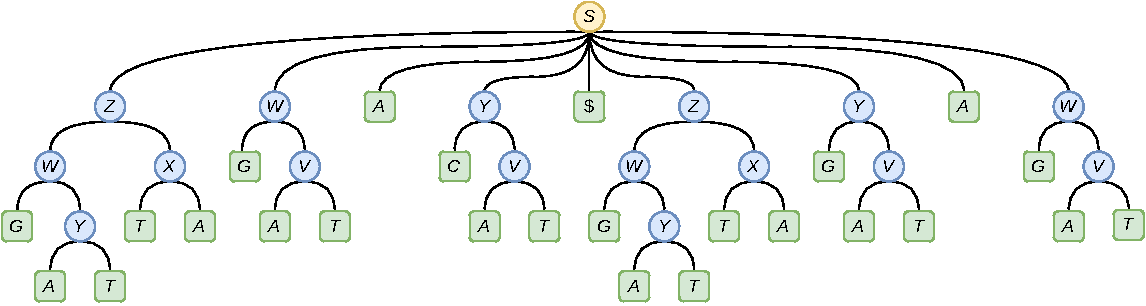
\includegraphics[width=\textwidth]{img/slpgagie.pdf}
  \end{figure}
\end{esempio}
Nel 2020, Gagie et al. \cite{slpgagie}, a cui si rimanda per approfondimenti,
proposero una variante degli \textit{SLPs} che garantisse miglioramenti
prestazionali per il \textit{random access} alla grammatica stessa. Sfruttando,
ad esempio, i \textit{bit vector sparsi} si è quindi potuto garantire
\textit{random access} su un testo $T$, tale che $|T|=n$, compresso tramite
\textit{SLP}, in tempo:
\[\mathcal{O}(\log n)\]
\textbf{VERIFICARE BENE COSA SIA $n$}.\\
L'uso di tale variante degli \textit{SLP} è stato cruciale, come si vedrà più
avanti in questa tesi, per la costruzione della versione run-length encoded sia
della \textbf{Burrows-Wheeler Transform (\textit{BWT})} che della
\textbf{Positional Burrows-Wheeler Transform (\textit{PBWT})}.
\subsection{Longest Common Extension}
Oltre a permettere un veloce \textit{random access} alla testo compresso, la
variante degli \textit{SLPs} proposta da Gagie et al. permette di effettuare
un'altra operazione in modo ``veloce'': le \textbf{Longest Common Extension
  (\textit{LCE}) queries}.
\begin{definizione}
  Dato un testo $T$, tale che $|T|=n$, il risultato della \textbf{LCE query} tra
  due posizioni $i$ e $j$, tali che $0\leq i,j<n$, corrisponde al più lungo
  prefisso comune tra le sotto-stringhe che hanno come indice di partenza $i$ e
  $j$, avendo quindi il più lungo prefisso comune tra $T[i,n-1]$ e $T[j,n-1]$.
\end{definizione}
Sfruttando l'\textit{SLP} del testo $T$ è quindi possibile effettuare due
\textit{random access} al testo compresso, in $i$ e $j$, per poi ``risalire''
l'albero al fine di computare il prefisso comune tra $T[i,n-1]$ e
$T[j,n-1]$. Quindi il calcolo di una \textit{LCE query} di lunghezza $l$ è
effettuabile in tempo:
\[\mathcal{O}\left(1+\frac{l}{\log n}\right)\]
\textbf{VERIFICARE BENE COSA SIA $n$}.

% sezione suffix array
\section{Suffix Array}
Nel 1976, Manber e Myers \cite{sa} proposero una struttura dati per la
memorizzazione di 
stringhe e la loro interrogazione, efficiente sia in termini di uso della
memoria che di complessità temporale. Tale struttura venne nominata
\textbf{Suffix Array} ($\SA$).
\begin{definizione}
  Dato un testo $T$, \$-terminato (assumendo che il simbolo \$ sia sempre il
  simbolo lessicograficamente minore nell'alfabeto di studio), tale che $|T|=n$,
  si definisce suffix 
    array di $T$, denotato con $\SA_T$, un array di interi lungo $n$, tale che
  $\SA_T[i]=j$ sse il suffisso di ordine $j$, ovvero $T[j,n-1]$, è
  l'$i$-esimo suffisso nell’ordinamento lessicografico dei suffissi di $T$. Ne
  segue che, presi $i,i'\in \mathbb{N}$
  tali che $0\leq i < i' < n$ allora vale che, indicando con $\prec$
  l'ordinamento lessicografico:
  \begin{equation}
    \label{eq:saord}
    T[\SA_T[i],n-1] \prec T[\SA_T[i'],n-1]
  \end{equation}
  Il suffix array è quindi una permutazione dei numeri interi in
  $\{0,n-1\}$. 
\end{definizione}
\begin{esempio}
  Si prenda la stringa:
  \[s=\mbox{mississippi\$},\,\,|s|=12\]
  Si producono quindi i seguenti suffissi e il loro riordinamento:
  \begin{table}[H]
    \footnotesize
    \centering
    \begin{tabular}{c|l}
      \textbf{Indice del suffisso} & \textbf{Suffisso}\\
      \hline
      0 & mississippi\$\\
      1 & ississippi\$\\
      2 & ssissippi\$\\
      3 & sissippi\$\\
      4 & issippi\$\\
      5 & ssippi\$\\
      6 & sippi\$\\
      7 & ippi\$\\
      8 & ppi\$\\
      9 & pi\$\\
      10 & i\$\\
      11 & \$\\
    \end{tabular}
    \quad $\implies$\quad
    \begin{tabular}{c|l} 
      \textbf{Indice del suffisso} & \textbf{Suffisso}\\ 
      \hline
      11 & \$\\
      10 & i\$\\
      7 & ippi\$\\
      4 & issippi\$\\
      1 & ississippi\$\\
      0 & mississippi\$\\
      9 & pi\$\\
      8 & ppi\$\\
      6 & sippi\$\\
      3 & sissippi\$\\
      5 & ssippi\$\\
      2 & ssissippi\$\\
    \end{tabular}
  \end{table}
  Avendo che:
  \[\SA_T=[11,10,7,4,1,0,9,8,6,3,5,2]\]
\end{esempio}
\subsection{Longest common prefix}
L'uso del suffix array è spesso accompagnato da un'altra struttura
dati, detta \textbf{Longest Common Prefix} ($\LCP$).
\begin{definizione}
  Si definisce il Longest Common Prefix di un testo $T$
  lungo $n$,
  denotato con $\LCP_T$, come un array lungo $n+1$, contenente la
  lunghezza del prefisso comune tra ogni coppia di suffissi consecutivi
  nell'ordinamento lessicografico dei suffissi, ovvero l'ordinamento specificato
  da $\SA_T$. Più formalmente
  $\LCP_T$ è un array tale che, avendo $0\leq i\leq n$ e indicando con
  $\lcp(x,y)$ il più lungo prefisso comune tra le stringhe $x$ e $y$:
  \begin{equation}
    \label{eq:lcpdef}
    \LCP_T[i]=
    \begin{cases}
      -1&\mbox{ se } i=0 \lor i=n\\
      \big\lvert\lcp(T[\SA_T[i-1], n],T[\SA_T [i], n])\big\rvert&\mbox{
        altrimenti} 
    \end{cases}
  \end{equation}
\end{definizione}
\begin{esempio}
  Riprendendo l'esempio precedente si avrebbe quindi:
  \begin{table}[H]
    \centering
    \footnotesize
    \begin{tabular}{c|c|c|l} 
      \textbf{Indice} & $\SA_T$ & $\LCP_T$ & \textbf{Suffisso}\\ 
      \hline
      0 & 11 & -1 & \$\\
      1 & 10 & 0 & i\$\\
      2 & 7 & 1 & \underline{i}ppi\$\\
      3 & 4 & 1 & \underline{i}ssippi\$\\
      4 & 1 & 4 & \underline{issi}ssippi\$\\
      5 & 0 & 0 & mississippi\$\\
      6 & 9 & 0 & pi\$\\
      7 & 8 & 1 & \underline{p}pi\$\\
      8 & 6 & 0 & sippi\$\\
      9 & 3 & 2 & \underline{si}ssippi\$\\
      10 & 5 & 1 & \underline{s}sippi\$\\
      11 & 2 & 3 & \underline{ssi}ssippi\$\\
      12 & - & -1 & -
    \end{tabular}
  \end{table}
\end{esempio}
Senza entrare in ulteriori dettagli relativi all'algoritmo di pattern matching
tramite $\SA$ e $\LCP$, in quanto non centrali per il resto della
trattazione, risulta comunque interessante riportare le complessità
temporali. Si ha che, per l'algoritmo di query su $\SA$ senza l'uso
dell'$\,\LCP$, si ha, per un testo lungo $n$ e un pattern lungo $m$:
\begin{equation}
  \label{eq:satime}
  \mathcal{O}(m\log n)
\end{equation}
Con l'uso dell'$\,\LCP$, si riduce a:
\begin{equation}
  \label{eq:salcptime}
  \mathcal{O}(m+\log n)
\end{equation}
Per ulteriori approfondimenti in merito agli algoritmi di pattern matching
basati su suffix array e ai relativi ``acceleratori'', si rimanda
al testo di Gusfield \cite{gusfield1997}.
\subsection{Inverse suffix array}
Ai fini di poter comprendere future definizioni si presenta anche la
permutazione inversa dei valori del suffix array, detta
\textbf{Inverse Suffix Array} ($\ISA$). Grazie a tale permutazione
inversa, dato un indice di suffisso, è possibile sapere in quale posizione si
trovi tale suffisso nel \textit{suffix array}.  
\begin{definizione}
  Dato il suffix array $\SA_T$, costruito su un testo $T$ di lunghezza
  $n$, si definisce l'inverse suffix array, denotato con $\ISA_T$, come:
  \begin{equation}
    \label{eq:isadef}
    \ISA_T[i]=j\iff \SA_T[j]=i,\,\,\forall\, i\in\{0,n-1\}
  \end{equation}
\end{definizione}

\begin{esempio}
  Riprendendo l'esempio precedente si avrebbe quindi:
  \begin{table}[H]
    \centering
    \footnotesize
    \begin{tabular}{c|c|c|l} 
      \textbf{Indice} & $\SA_T$ & $\ISA_T$ & \textbf{Suffisso}\\ 
      \hline
      0 & 11 & 5 & \$\\
      1 & 10 & 4 & i\$\\
      2 & 7 & 11 & ippi\$\\
      3 & 4 & 9 & issippi\$\\
      4 & 1 & 3 & ississippi\$\\
      5 & 0 & 10 & mississippi\$\\
      6 & 9 & 8 & pi\$\\
      7 & 8 & 2 & ppi\$\\
      8 & 6 & 7 & sippi\$\\
      9 & 3 & 6 & sissippi\$\\
      10 & 5 & 1 & ssippi\$\\
      11 & 2 & 0 & ssissippi\$\\
    \end{tabular}
  \end{table}
\end{esempio}
\subsection{Permuted longest common prefix}
Un'altra permutazione che bisogna introdurre è il \textbf{permuted
  longest common prefix} ($\PLCP$) \textbf{array} \cite{plcp}.
Tale permutazione
permette una rappresentazione succinta in memoria dell'$\,\LCP$ \cite{plcp2},
permettendo di ottenere gli stessi risultati di quest'ultimo.
% Un'altro vantaggio
% è che la sua ricostruzione richiede un minor costo computazionale
.
\dc{L'intera sottosezione potrebbe essere quasi totalmente rimossa ma almeno la
  definizione serve per il calcolo di tutte le occorrenze di un MEM, come in
  PHONI} 
\begin{definizione}
  Si definisce il permuted longest common prefix, denotato con
  $\PLCP_T$, costruito a partire da un testo $T$ di lunghezza $n$, come un
  array tale per cui \cite{phoni}:
  \begin{equation}
    \label{eq:plcpdef1}
    \PLCP_T[p]=
    \begin{cases}
      -1&\mbox{se }\ISA_T[p]=0\\
     \LCP_T[\ISA_T[p]]&\mbox{altrimenti}
    \end{cases},\,\,\forall\, p\in\{0,n-1\}
  \end{equation}
  Si noti che i valori sono in ordine di posizione, ovvero l'ordine originale
  dato dagli indici dei suffissi, e non
  lessicografico. In altri termini, si ha una permutazione dei valori di $\LCP_T$
  tale per cui \cite{plcp}:
  \begin{equation}
    \label{eq:plcpdef2}
    \PLCP_T[\SA_T[p]] = \LCP_T[p],\,\,\,\forall\, p\in\{1,n-1\}
  \end{equation}
\end{definizione}
\begin{esempio}
  Riprendendo l'esempio precedente si avrebbe quindi:
  \begin{table}[H]
    \centering
    \footnotesize
    \begin{tabular}{c|c|c|c|c|l} 
      \textbf{Indice} & $\SA_T$ & $\ISA_T$ & $\LCP_T$
      & $\PLCP_T$ & \textbf{Suffisso}\\  
      \hline
      0 & 11 & 5 & -1 & 0 & \$\\
      1 & 10 & 4 & 0 & 4 & i\$\\
      2 & 7 & 11 & 1 & 3 & \underline{i}ppi\$\\
      3 & 4 & 9 & 1 & 2 & \underline{i}ssippi\$\\
      4 & 1 & 3 & 4 & 1 & \underline{issi}ssippi\$\\
      5 & 0 & 10 & 0 & 1 & mississippi\$\\
      6 & 9 & 8 & 0 & 0 & pi\$\\
      7 & 8 & 2 & 1 & 1 & \underline{p}pi\$\\
      8 & 6 & 7 & 0 & 1 & sippi\$\\
      9 & 3 & 6 & 2 & 0 & \underline{si}ssippi\$\\
      10 & 5 & 1 & 1 & 0 & \underline{s}sippi\$\\
      11 & 2 & 0 & 3 & -1 & \underline{ssi}ssippi\$\\
      12 & - & - & -1 & - & - 
    \end{tabular}
  \end{table}
\end{esempio}
Ciò che permette una rappresentazione compatta del \textit{PLCP} è descritto nel
seguente lemma \cite{plcp3}.
\begin{lemma}
  Dato un testo $T$, tale che $|T|=n$, si ha che:
  \begin{equation}
    \label{eq:plcpdef3}
    \PLCP_T[i]\geq \PLCP_T[i-1]-1,\,\,\forall\, i\in\{1,n-1\}
  \end{equation}
\end{lemma}
Grazie a tale lemma si può memorizzare l'$\,\PLCP$ sparso.
\begin{definizione}
  Dato un intero
  $q$, per il quale calcolo (basato sul lemma precedente) si rimanda al paper di
  Kasai \cite{plcp3}, si definisce array $\PLCP$ sparso, lungo
  $\left\lfloor\frac{n}{q}\right\rfloor$ e denotato $\PLCP_q$, come l'array che
  memorizza ogni $q$-esimo valore del $\PLCP$, avendo che:
  \begin{equation}
    \label{eq:plcpdef4}
    \PLCP_q[i]=\PLCP_T[iq]
  \end{equation}
\end{definizione}
\dc{Capire se serve variante sparsa e se serve esempio}
\subsection{Funzione phi}
L'ultimo concetto che si introduce sono le \textbf{funzioni}
$\boldsymbol\varphi$ e $\mathbf{\boldsymbol\varphi^{-1}}$, usate per poter
identificare i valori precedenti e successivi di 
un dato valore in $\SA_T$. Essere sono utili al fine di poter sia ricostruire
efficientemente il $\PLCP$ di un testo $T$ (per i dettagli si rimanda
all'articolo di K\"{a}rkk\"{a}inen \cite{plcp}) che di permettere, come si vedrà
più  avanti nella sezione \ref{secbwt}, il riconoscimento di tutte le occorrenze
di un \textbf{maximal exact match} ($\MEM$) in $T$ \cite{phoni}.
\begin{definizione}
  Dato un testo $T$ di lunghezza $n$ si definiscono le funzioni, che di fatto
  sono permutazioni dei valori di $\SA_T$, $\varphi$ e
  $\varphi^{-1}$ come \cite{phoni}: 
  \begin{equation}
    \label{eq:phidef1}
    \varphi(p)=
    \begin{cases}
      \NULL&\mbox{se } \ISA_T[p]=0\\
      \SA_T[\ISA_T[p]-1]&\mbox{altrimenti}
    \end{cases},\,\,\forall\, p\in\{0,n-1\}
  \end{equation}
  \begin{equation}
    \label{eq:phiinvdef1}
    \varphi^{-1}(p)=
    \begin{cases}
      \NULL&\mbox{se } \ISA_T[p]=n-1\\
      \SA_T[\ISA_T[p]+1]&\mbox{altrimenti}
    \end{cases},\,\,\forall\, p\in\{0,n-1\}
  \end{equation}
  Si noti che si ha il valore $\NULL$ quando, rispettivamente, si studia il
  primo e l'ultimo valore del \textit{suffix array} in quanto non hanno, sempre
  rispettivamente, l'antecedente e il successore. Infatti, tali
  funzioni restituiscono i due valori, se 
  esistenti, di $\SA_T$ adiacenti ad un valore del suffix array dato.\\
  Analogamente, sempre coi medesimi vincoli, le due funzioni possono essere
  definite come \cite{plcp}: 
  \begin{equation}
    \label{eq:phidef2}
    \varphi(\SA[p])=\SA[p-1]
  \end{equation}
  \begin{equation}
    \label{eq:phiinvdef2}
    \varphi^{-1}(\SA[p])=\SA[p+1]
  \end{equation}

\end{definizione}
\begin{esempio}
   Riprendendo l'esempio precedente si avrebbe quindi:
   % \begin{table}[H]
   %   \centering
   %   \footnotesize
   %   \begin{tabular}{c|c|c|c|c|c|c|l} 
   %     \textbf{Indice} & $\mathbf{SA_T}$ & $\mathbf{ISA_T}$ & $\mathbf{LCP_T}$
   %     & $\mathbf{PLCP_T}$ & $\mathbf{\boldsymbol\varphi}$
   %     & $\mathbf{\boldsymbol\varphi^{-1}}$ & \textbf{Suffisso}\\  
   %     \hline
   %     0 & 11 & 5 & -1 & 0 & 1 & 9 & \$\\
   %     1 & 10 & 4 & 0 & 4 & 4 & 0 & i\$\\
   %     2 & 7 & 11 & 1 & 3 & 5 & $null$ & ippi\$\\
   %     3 & 4 & 9 & 1 & 2 & 6 & 5 & issippi\$\\
   %     4 & 1 & 3 & 4 & 1 & 7 & 1 & ississippi\$\\
   %     5 & 0 & 10 & 0 & 1 & 3 & 2 & mississippi\$\\
   %     6 & 9 & 8 & 0 & 0 & 8 & 3 & pi\$\\
   %     7 & 8 & 2 & 1 & 1 & 10 & 4 & ppi\$\\
   %     8 & 6 & 7 & 0 & 1 & 9 & 6 & sippi\$\\
   %     9 & 3 & 6 & 2 & 0 & 0 & 8 & sissippi\$\\
   %     10 & 5 & 1 & 1 & 0 & 11 & 7 & ssippi\$\\
   %     11 & 2 & 0 & 3 & 0/-1 & $null$ & 10 & ssissippi\$\\
   %   \end{tabular}
   % \end{table}
   \begin{table}[H]
     \centering
     \footnotesize
     \begin{tabular}{c|c|c|c|c|l} 
       \textbf{Indice} & $\SA_T$ & $\ISA_T$
       & $\varphi$
       & $\varphi^{-1}$ & \textbf{Suffisso}\\  
       \hline
       0 & 11 & 5 & 1 & 9 & \$\\
       1 & 10 & 4 & 4 & 0 & i\$\\
       2 & 7 & 11 & 5 & $\NULL$ & ippi\$\\
       3 & 4 & 9 & 6 & 5 & issippi\$\\
       4 & 1 & 3 & 7 & 1 & ississippi\$\\
       5 & 0 & 10 & 3 & 2 & mississippi\$\\
       6 & 9 & 8 & 8 & 3 & pi\$\\
       7 & 8 & 2 & 10 & 4 & ppi\$\\
       8 & 6 & 7 & 9 & 6 & sippi\$\\
       9 & 3 & 6 & 0 & 8 & sissippi\$\\
       10 & 5 & 1 & 11 & 7 & ssippi\$\\
       11 & 2 & 0 & $\NULL$ & 10 & ssissippi\$\\
     \end{tabular}
   \end{table}
  Infatti, ad esempio, il valore $9$ in $\SA_T$ è preceduto dal valore
  $\varphi(9)=0$ ed è seguito dal valore $\varphi^{-1}(9)=8$.
\end{esempio}


% sezione BWT
\section{Trasformata di Burrows-Wheeler}
\label{secbwt}
Introdotta nel 1994 da Burrows e Wheeler con lo scopo di comprimere testi, la
\textbf{Burrows-Wheeler Transform} ($\BWT$) \cite{bwt} è divenuta ormai uno
standard nel 
campo dell'algoritmica su stringhe e della bioinformatica,
grazie ai suoi molteplici vantaggi sia dal punto di vista della complessità
temporale che da quello dell'efficienza in memoria.\\
Nel dettaglio la $\BWT$ è una trasformata reversibile che
permette una compressione lossless, quindi senza perdita
d'informazione. Tale trasformazione viene costruita a partire dal riordinamento
dei caratteri del testo in input, riordinando lessicograficamente le cosiddette
\textit{rotazioni} del testo. Interessante è la proprietà per cui caratteri
uguali tendono ad essere posti consecutivamente all'interno della stringa
prodotta dalla trasformata. Questa proprietà è causata dalle ripetizioni di
sottostringhe all'interno del testo stesso.
\begin{definizione}
  Dato un testo $T$ \$-terminato, tale che $|T|=n$, si definisce la
  Burrows--Wheeler Transform di $T$, denotata con
  $\BWT_T$, come un array di caratteri lungo $n$ dove l'elemento $i$-esimo è il
  carattere che precede l'$i$-esimo suffisso $T$ nel riordinamento
  lessicografico. Più formalmente si ha che:
  \begin{equation}
    \label{eq:bwt1}
    \BWT_T[i]=
    \begin{cases}
      T[\SA_T[i]-1]&\mbox{ se } \SA_T[i]\neq 1\\
      \$&\mbox{ altrimenti}
    \end{cases},\,\, \forall\, i\in\{0,n-1\}
  \end{equation}
\end{definizione}
In termini operativi, la $\BWT$ di un testo è calcolabile riordinando
lessicograficamente tutte le possibili rotazioni del testo $T$.
\begin{definizione}
  Si definisce rotazione $i$-esima di
  un testo $T$ lungo $n$, denotata con $\ROT_T(i)$, come la stringa ottenuta
  dalla concatenazione 
  del suffisso $i$-esimo con la restante porzione del testo. Più formalmente si
  ha che, denotando con $X\cdot Y$ la concatenazione tra
  la stringa $X$ e la stringa $Y$:
  \begin{equation}
    \label{eq:bwt2}
    \ROT_T(i)=T[i,n-1]\cdot T[0,i-1],\,\,\forall\, i\in\{0,n-1\}
  \end{equation}
\end{definizione}
Data questa definizione, quindi, la $\BWT$ del testo $T$ risulta essere
l'ultima colonna della matrice, detta \textbf{Burrows--Wheeler Matrix} ($\BWM$),
che si ottiene riordinando tutte le  
rotazioni di $T$, che altro non sono che i suffissi già riordinati per
il calcolo di $\SA_T$ a cui viene concatenata la parte restante del
testo.\\
Un altro array spesso utilizzato insieme alla $\BWT$ è il cosiddetto
array $\F$, lungo $|T|$, che è l'array formato
dalla prima colonna della $\BWM$. In pratica l'array $\F_T$ è,
banalmente, l'array formato dal riordinamento 
lessicografico dei caratteri del testo $T$.
\begin{esempio}
  Si prenda la stringa:
  \[s=\mbox{mississippi\$},\,\,|s|=12\]
  Si produce la $\BWM_T$, da cui si estraggono $\F_T$ e $\BWT_T$:
  \begin{table}[H]
    \centering
    \footnotesize
    \begin{tabular}{c|c|c|c|c} 
      \textbf{Indice} & $\SA_T$ & $\F_T$ & $\BWM_T$
      & $\BWT_T$\\ 
      \hline
      0 & 11 & \$ & \$mississippi & i\\
      1 & 10 & i & i\$mississipp & p\\
      2 & 7 & i & ippi\$mississ & s\\
      3 & 4 & i & issippi\$miss & s\\
      4 & 1 & i & ississippi\$m & m\\
      5 & 0 & m & mississippi\$ & \$\\
      6 & 9 & p & pi\$mississip & p\\
      7 & 8 & p & ppi\$mississi & i\\
      8 & 6 & s & sippi\$missis & s\\
      9 & 3 & s & sissippi\$mis & s\\
      10 & 5 & s & ssippi\$missi & i\\
      11 & 2 & s & ssissippi\$mi & i\\
    \end{tabular}
  \end{table}
\end{esempio}
L'importanza di questa trasformata è dovuta soprattutto al fatto che sia
reversibile, implicando quindi che, a partire da $\BWT_T$, sia possibile
ricostruire $T$. Questo è possibile grazie ad una proprietà intrinseca della
trasformata che viene riassunta nel concetto di \textbf{LF-mapping}.
\begin{definizione}
  Dato un testo $T$, tale che $|T|=n$, data la sua $\BWT_T$ e il suo array
  $\F_T$ 
  si definisce LF-mapping come la proprietà per la quale l'$i$-esima
  occorrenza di un carattere $\sigma$ in $\BWT_T$ corrisponde all'$i$-esima
  occorrenza dello stesso carattere in $\F_T$.
\end{definizione}
Grazie a questa definizione è possibile partire dall'ultimo carattere del testo,
ovvero $\sigma=\$$, e ricostruire l'intero testo a ritroso. Si vede quindi un
breve esempio. 
\begin{esempio}
  Si riprende l'esempio precedente, avendo:
  \[\BWT_T=\mbox{ipssm\$pissii}\mbox{ e }\F_T=\mbox{\$iiiimppssss}\]
  E avendo i seguenti caratteri associati dall'\textit{LF-mapping}:
  \begin{figure}[H]
    \centering
    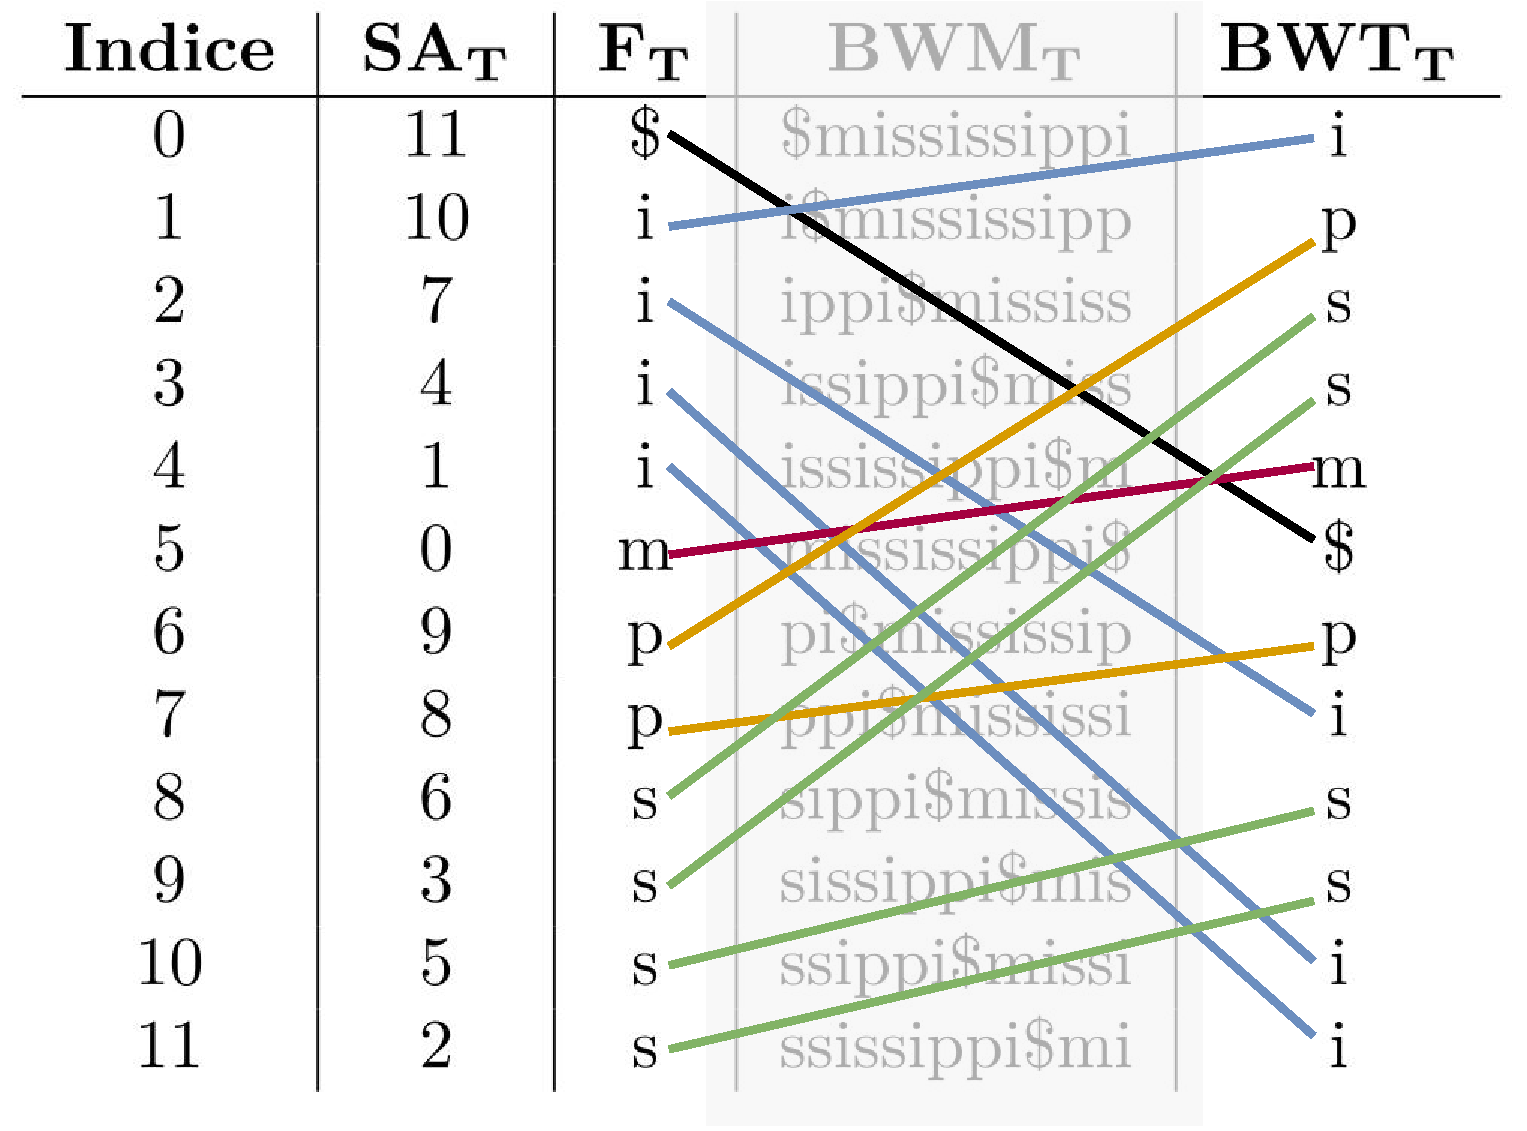
\includegraphics[scale = 0.33]{img/lf.pdf}
  \end{figure}
  Si comincia dal simbolo '\$' in $\BWT_T$, che è l'ultimo carattere di $T$. Si
  ha che esso corrisponde al primo e unico simbolo '\$' in $\F_T$, all'indice
  $0$. Tale simbolo, per l'ovvia proprietà delle rotazioni è preceduto dal
  simbolo $\BWT_T[0]=\mbox{'i'}$ in $T$. Quindi $\mbox{'i'}$ precederà '\$' in
  $T$:
  \[T=\ldots\mbox{i\$}\]
  Si sa inoltre che
  tale $\mbox{'i'}$ è il primo $\mbox{'i'}$ in $\BWT_T$. Si cerca quindi il
  primo simbolo $\mbox{'i'}$ anche in $\F_T$,
  sapendo che sono lo stesso simbolo nel testo. A questo punto il simbolo allo
  stesso indice di tale $\mbox{'i'}$ nella $\BWT_T$, ovvero il simbolo
  $\mbox{'p'}$, sarà il simbolo che precede $\mbox{'i'}$ nel testo:
  \[T=\ldots\mbox{pi\$}\]
  Proseguendo a ritroso si ricostruisce l'intero testo:
  \[T=\mbox{mississippi\$}\]
\end{esempio}
\dc{Questo esempio serve davvero?}
\subsubsection{FM-index}
Tramite l'uso dell'LF-mapping è possibile risolvere il problema di
ricerca di un pattern all'interno del testo, tramite l'algoritmo nominato
\textbf{backward search}. Questa tecnica consiste nell'iterare il pattern da
destra a sinistra e
salvare, di volta in volta, un intervallo sul suffix array. Nel
dettaglio, ipotizzando di essere in posizione $i$ del pattern, tale
intervallo è relativo a quei suffissi che hanno come prefisso il suffisso
$i$-esimo del pattern. Tale intervallo viene esteso usando il carattere
$P[i-1]$ selezionando il nuovo intervallo sul suffix array. Tale
aggiornamento è detto \textit{backward step} e consiste nell'aggiornare
l'intervallo sul suffix array a quei suffissi del testo che, estesi a sinistra
col carattere $(i-1)$-esimo del pattern, presentano un match con $P[i-1,
|P|-1]$.\\   
Usando la $\BWT$ è possibile usare due funzioni, dette $\C$ e $\Occ$, per
computare la backward search.
\begin{definizione}
  Dato un testo \$-terminato $T$, lungo $n$ e costruito su alfabeto $\Sigma$, si
  definisce la funzione $\C$, come una funzione:
  \begin{equation}
    \label{eq:bwt4}
    \C:\Sigma\cup \$\to \mathbb{N}
  \end{equation}
  Dato un carattere $\sigma\in\Sigma$, $\C(\sigma)$ restituisce il
  numero di 
  occorrenze dei caratteri lessicograficamente più piccoli di $\sigma$ in $T$.
\end{definizione}
\begin{definizione}
  Dato un testo \$-terminato $T$, lungo $n$ e costruito su alfabeto $\Sigma$, e
  la sua $BWT_T$, si definisce la funzione $\Occ$, come una funzione:
  \begin{equation}
    \label{eq:bwt5}
    \Occ:\Sigma\cup \$\times \{0,n\}\to \mathbb{N}
  \end{equation}
  Dato un carattere $\sigma\in\Sigma$ e una posizione $i$ della
  $BWT_T$, $\Occ(\sigma,i)$ restituisce il numero di occorrenze del carattere
  $\sigma$ nei primi $i$ elementi di $\BWT_T$.
\end{definizione}
Questa coppia di funzioni prende il nome di \textbf{FM-index} \cite{fm}, il
quale è definito essere un self index in quanto è possibile tenere in
memoria solo tale indice per ottenere i risultati medesimi della $\BWT_T$,
ricordando anche che da essa si può ricostruire il testo $T$.
\begin{esempio}
  Si prenda la stringa:
  \[T=\mbox{mississippi\$},\,\,|s|=12\]
  Che produce:
  \[\BWT_T=\mbox{ipssm\$pissii}\]
  Si ha, per $\C(\sigma)$:
  \begin{table}[H]
    \centering
    \begin{tabular}{c||c}
      $\sigma$ & $\C(\sigma)$\\
      \hline
      \hline
      \$ & 0\\
      i & 1 \\
      m & 5\\
      p & 6\\
      s & 8\\
    \end{tabular}
  \end{table}
  Per $\Occ(\sigma, i)$, si ha:
  \begin{table}[H]
    \centering
    \begin{tabular}{c||c|c|c|c|c}
      0 & 0 & 0 & 0 & 0 & 0 \\
      1 & 0 & 1 & 0 & 0 & 0 \\
      2 & 0 & 1 & 0 & 1 & 0 \\
      3 & 0 & 1 & 0 & 1 & 1 \\
      4 & 0 & 1 & 0 & 1 & 2 \\
      5 & 0 & 1 & 1 & 1 & 2 \\
      6 & 1 & 1 & 1 & 1 & 2 \\
      7 & 1 & 1 & 1 & 2 & 2 \\
      8 & 1 & 2 & 1 & 2 & 2 \\
      9 & 1 & 2 & 1 & 2 & 3 \\
      10 & 1 & 2 & 1 & 2 & 4 \\
      11 & 1 & 3 & 1 & 2 & 4 \\
      12 & 1 & 4 & 1 & 2 & 4 \\
      \hline
      \hline
      i/$\sigma$ & \$ & i & m & p & s
    \end{tabular}
  \end{table}
\end{esempio}
Dato un simbolo $\sigma$ del pattern e il precedente intervallo $[f,g)$ su
$\SA_T$, si esegue il backward step, tramite l'FM-index,
aggiornando $f$ e $g$ nel seguente modo: 
\begin{equation}
  \label{eq:bwt6}
  f'=\C(\sigma)+\Occ(\sigma, f),\quad g'=\C(\sigma)+\Occ(\sigma, g)
\end{equation}
Ritornando il nuovo intervallo $[f, g)\gets [f', g')$ sse $f'< g'$.
Si segnala che tali variabili sono inizializzate con $f=0$ e $g=n$.\\
Tale calcolo altro non è che l'LF-mapping. Infatti, partendo da un
intervallo su $\SA_T$ (che è anche un intervallo su $\BWT_T$), si identificano
quali suffissi sono preceduti dal simbolo del pattern voluto. Tale simbolo, se
il 
pattern ha un'occorrenza fino al carattere in analisi, sarà presente in
sottointervallo di $[f,g)$ sulla $\BWT_T$. Una volta identificati tali caratteri
su $\BWT_T$ si usano $\C(\sigma)$ e $\Occ(\sigma, i)$, per trovare tali
caratteri su $\F_T$, calcolando il nuovo intervallo $[f,g)$.
\dc{capire se dire meglio}
\begin{esempio}
  Si assuma il pattern $P=\mbox{iss}$ da voler ricercare nel testo
  $T=\mbox{mississippi\$}$. 
  Si ha, in termini di inizializzazione che $f=0$, $g=12$,
  $\sigma=P[|P|-1]=P[2]=s$. Si calcolano i nuovi $f'$ e $g'$:
  \[f'=\C(s)+\Occ(s, 0)=8+0=8\]
  \[g'=\C(s)+\Occ(s, 12)=8+4=12\]
  Ottenendo l'intervallo $[8,12)$ sul suffix array.\\
  Si prosegue leggendo il carattere $\sigma=P[1]=s$:
  \[f'=\C(s)+\Occ(s, 8)=8+2=10\]
  \[g'=\C(s)+\Occ(s, 12)=8+4=12\]
  Limitando quindi l'intervallo a $[10,12)$. Si noti che tale intervallo
  corrisponde ai due simboli ``s'' presenti in $\BWT_T[8,11]$, che sono
  esattamente i simboli in $\F_T[10,11]$.
  Un ulteriore aggiornamento, col carattere $\sigma=P[0]=i$, comporta:
  \[f'=\C(i)+\Occ(i, 10)=1+2=3\]
  \[g'=\C(i)+\Occ(i, 12)=1+4=5\]
  Avendo l'intervallo finale su $\SA_T$ del match, ovvero: $[3,5)$.
  Seguendo l'intero ragionamento sul \textit{suffix array} si avrebbe:
  \begin{table}[H]
    \centering
    \scriptsize
    \begin{tabular}{c|c|c|c|c} 
      \textbf{Indice} & $\SA_T$ & $\F_T$ & $\BWM_T$
      & $\BWT_T$\\ 
      \hline
      {\color{nordred}{0}} & 11 & \$ & {\color{nordred}{\$}}mississippi & i\\
      {\color{nordred}{1}} & 10 & i & {\color{nordred}{i}}\$mississipp & p\\
      {\color{nordred}{2}} & 7 & i & {\color{nordred}{i}}ppi\$mississ
      & {\color{nordgreen}{s}}\\
      {\color{nordred}{3}} & 4 & i & {\color{nordred}{i}}ssippi\$miss
      & {\color{nordgreen}{s}}\\
      {\color{nordred}{4}} & 1 & i & {\color{nordred}{i}}ssissippi\$m & m\\
      {\color{nordred}{5}} & 0 & m & {\color{nordred}{m}}ississippi\$ & \$\\
      {\color{nordred}{6}} & 9 & p & {\color{nordred}{p}}i\$mississip & p\\
      {\color{nordred}{7}} & 8 & p & {\color{nordred}{p}}pi\$mississi & i\\
      {\color{nordred}{8}} & 6 & s & {\color{nordred}{s}}ippi\$missis
      & {\color{nordgreen}{s}}\\
      {\color{nordred}{9}} & 3 & s & {\color{nordred}{s}}issippi\$mis
      & {\color{nordgreen}{s}}\\
      {\color{nordred}{10}} & 5 & s & {\color{nordred}{s}}sippi\$missi & i\\
      {\color{nordred}{11}} & 2 & s & {\color{nordred}{s}}sissippi\$mi & i\\
    \end{tabular}
    $\implies$
    \begin{tabular}{c|c|c|c|c} 
      \textbf{Indice} & $\SA_T$ & $\F_T$ & $\BWM_T$
      & $\BWT_T$\\  
      \hline
      0 & 11 & \$ & \$mississippi & i\\
      1 & 10 & i & i\$mississipp & p\\
      2 & 7 & i & ippi\$mississ & s\\
      3 & 4 & i & issippi\$miss & s\\
      4 & 1 & i & ississippi\$m & m\\
      5 & 0 & m & mississippi\$ & \$\\
      6 & 9 & p & pi\$mississip & p\\
      7 & 8 & p & ppi\$mississi & i\\
      {\color{nordred}{8}} & 6 & s & {\color{nordred}{s}}ippi\$missis
      & {\color{nordgreen}{s}}\\
      {\color{nordred}{9}} & 3 & s & {\color{nordred}{s}}issippi\$mis
      & {\color{nordgreen}{s}}\\
      {\color{nordred}{10}} & 5 & s & {\color{nordred}{s}}sippi\$missi & i\\
      {\color{nordred}{11}} & 2 & s & {\color{nordred}{s}}sissippi\$mi & i\\
    \end{tabular}
  \end{table}
  \[\Downarrow\]
  \begin{table}[H]
    \centering
    \scriptsize
    \begin{tabular}{c|c|c|c|c} 
    \textbf{Indice} & $\SA_T$ & $\F_T$ & $\BWM_T$
      & $\BWT_T$\\ 
      \hline
      0 & 11 & \$ & \$mississippi & i\\
      1 & 10 & i & i\$mississipp & p\\
      2 & 7 & i & ippi\$mississ & s\\
      3 & 4 & i & issippi\$miss & s\\
      4 & 1 & i & ississippi\$m & m\\
      5 & 0 & m & mississippi\$ & \$\\
      6 & 9 & p & pi\$mississip & p\\
      7 & 8 & p & ppi\$mississi & i\\
      8 & 6 & s & sippi\$missis & s\\
      9 & 3 & s & sissippi\$mis & s\\
      {\color{nordred}{10}} & 5 & s & {\color{nordred}{ss}}ippi\$missi
      & {\color{nordgreen}{i}}\\
      {\color{nordred}{11}} & 2 & s & {\color{nordred}{ss}}issippi\$mi
      & {\color{nordgreen}{i}}\\
    \end{tabular}
    $\implies$
    \begin{tabular}{c|c|c|c|c} 
      \textbf{Indice} & $\SA_T$ & $\F_T$ & $\BWM_T$
      & $\BWT_T$\\ 
      \hline
      0 & 11 & \$ & \$mississippi & i\\
      1 & 10 & i & i\$mississipp & p\\
      2 & 7 & i & ippi\$mississ & s\\
      {\color{nordred}{3}} & {\color{nordgreen}{\underline{4}}} & i
                                        & {\color{nordred}{iss}}ippi\$miss & s\\
      {\color{nordred}{4}} & {\color{nordgreen}{\underline{1}}} & i
                                        & {\color{nordred}{iss}}issippi\$m & m\\
      5 & 0 & m & mississippi\$ & \$\\
      6 & 9 & p & pi\$mississip & p\\
      7 & 8 & p & ppi\$mississi & i\\
      8 & 6 & s & sippi\$missis & s\\
      9 & 3 & s & sissippi\$mis & s\\
      10 & 5 & s & ssippi\$missi & i\\
      11 & 2 & s & ssissippi\$mi & i\\
    \end{tabular}
  \end{table}
  Avendo quindi che le occorrenze del pattern $P=\mbox{iss}$ iniziano alle
  posizioni $\SA_T[3]=4$ e $\SA_T[4]=1$ del testo.
\end{esempio}
\section{Trasformata di Burrows--Wheeler run-length encoded}
Come già introdotto, la $\BWT$ tende ad avere caratteri uguali in
posizioni consecutive all'interno della sua sequenza. Si è quindi 
pensato, fin da subito, ad un modo efficiente per memorizzare in modo compresso
testi mediante l'uso del run-length encoding. Tale tecnica consiste nel
memorizzare le cosiddette run, ovvero sequenze massimali di caratteri
uguali, mediante coppie: 
\[(\mbox{carattere}, \mbox{lunghezza della run})\]
\begin{esempio}
  Vediamo un breve esempio.\\
  Si ipotizzi di avere la seguente stringa:
  \[s=\mbox{aaaacctgggggg}\]
  Una sua memorizzazione run-length sarebbe del tipo:
  \[\{(a,4),(c,2),(t,1),(g,6)\}\]
\end{esempio}
\subsection{RLBWT e r-index}
In questa direzione, nel 2005, M\"{a}niken e Navarro proposero la
\textbf{Run-Length encoded Burrows-–Wheeler Transform} ($\RLBWT$)
\cite{rlbwt}.
\begin{definizione}
  Dato un testo $T$ si definisce la \RLBWT di $T$
  come la rappresentazione run-length encoded della $\BWT_T$,
  denotandola con $\RLBWT_T$. Si noti che, avendo $r$ come numero di run nella
  $\BWT_T$: 
  \begin{equation}
    \label{eq:rlbwt1}
    |\RLBWT_T|=r
  \end{equation}
\end{definizione}
L'uso di tale
struttura risulta particolarmente efficiente, ad esempio, volendo creare
un'unica $\BWT$ a partire dalla concatenazione di multipli
genomi. Infatti, tale
concatenazione conterrà, per ovvie ragioni biologiche, diverse regioni genomiche
ripetute. \\
Una strategia per la memorizzazione in modo compatto la $\RLBWT$ è quella
di memorizzare: 
\begin{itemize}
  \item una stringa $c$, tale che $|c|=r$, contenente un solo carattere per ogni
  run della $\BWT_T$
  \item un bitvector $bv$, lungo quanto $\BWT_T$, tale che $bv[i]=1$ sse
  $\BWT_T[i]$ è il primo carattere, detto anche testa, di una run 
\end{itemize}
\begin{esempio}
  Si prenda ad esempio la seguente $\BWT_T$:
  \[\BWT_T=acggtcccaa\]
  Si hanno:
  \[c=acgtca\quad \quad bv=1110110010\]
\end{esempio}
M\"{a}niken e Navarro hanno proposto anche il seguente teorema.
\begin{teorema}
  Dato un testo $T$, tale che $|T|=n$, si costruire $\RLBWT_T$ in
  uno spazio $\mathcal{O}(r)$ tale per cui si possono conteggiare tutte le
  occorrenze di un pattern $P$, tale che $|P|=m$, in tempo:
  \begin{equation}
    \label{eq:rlbwt2}
    \mathcal{O}(m\log n)
  \end{equation}
\end{teorema}
\noindent
La struttura dati dietro questo risultato ha preso il nome di \textbf{r-index}.
Tale indice consiste in: 
\begin{itemize}
  \item la $\RLBWT$
  \item dei suffix array sample, in spazio $\mathcal{O}(r)$
\end{itemize}
Grazie a tale indice, dato un testo $T$, tale che
$|T|=n$, e dato un pattern $P$, tale che $|P|=m$, è stato possibile: 
\begin{itemize}
  \item conteggiare le occorrenze (\textit{count query}) del pattern nel testo,
  in tempo $\mathcal{O}(m\log n)$ e in spazio $\mathcal{O}(r)$  
  \item localizzare tali occorrenze (\textit{locate query}) in tempo
  $\mathcal{O}(s)$ e in spazio $\mathcal{O}\left(\frac{r}{s}\right)$, avendo $s$
  come distanza tra due $\SA$ \textit{sample}
\end{itemize}
Nel 2017, Policriti and Prezza \cite{policriti} proposero un teorema
fondamentale in questo ambito.
\begin{teorema}[Toehold lemma]
  Dato un testo $T$, tale che $|T|=n$, e dato un pattern $P$, tale
  che $|P|=m$, si può computare l'intervallo sulla $\BWT_T$ contenente i $k$
  caratteri precedenti le occorrenze di $P$ in $T$ in spazio $\mathcal{O}(r)$ e
  in tempo: 
  \begin{equation}
    \label{eq:rlbwt3}
    \mathcal{O}(m\log\log n)
  \end{equation}
\end{teorema}
Questo risultato dimostra come identificare \underline{un} $\SA$ sample
nell'intervallo 
contenente il pattern $P$. Il limite è dato dal fatto che non si supporta la
localizzazione di tutte le $k$ occorrenze degli $\SA$ sample in
quell'intervallo.\\
Nel 2020 Gagie et al \cite{gagie2020}, combinando la $\RLBWT$, il
Toehold lemma e la già introdottta funzione $\varphi$, trovarono una soluzione a
questo problema, permettendo di avere le \textit{locate 
  query} in spazio $\mathcal{O}(r)$.
Tale risultato si riassume nel seguente teorema.
\begin{teorema}
  Dato un testo $T$, tale che $|T|=n$, si può memorizzare $T$ in spazio
  $\mathcal{O}(r)$ tale che si possano trovare tutte le $k$ occorrenze di un
  pattern $P$, lungo $m$, in tempo:
  \begin{equation}
    \label{eq:rlbwt4}
    \mathcal{O}((m+k)\log\log n)
  \end{equation}
\end{teorema}
Nel dettaglio, i risultati di Gagie portarono a ridefinire l'r-index
tramite l'uso dei valori del $\SA$ all'inizio e alla fine di ogni run come
$\SA$ sample. Si è quindi ottenuto che i $\SA$ sample possono
essere memorizzati in spazio proporzionale al numero di run, 
pur permettendo in modo efficiente le locate query.\\
Per ulteriori dettagli in merito alla costruzione dell'r-index si rimanda anche
ai 
paper di Kuhnle et al. \cite{kuhnle}, di Mun et al. \cite{mun} e di Boucher et
al. \cite{boucher}. 
\subsection{Match massimali con RLBWT}
Dopo aver introdotto l'r-index, bisogna brevemente come avvenga il
calcolo dei cosiddetti \textbf{Maximal Exact Match} ($\MEM$), ovvero match
esatti, tra un pattern e un testo, che non 
possono essere estesi in alcuna direzione, essendo quindi massimali.
\begin{definizione}
  Dato un testo $T$, con $|T|=n$, e un pattern $P$, con $|P|=m$, si definisce
  $\MEM$ di $P$ in $T$ una sottostringa $P[i,i+l-1]$, di lunghezza $l$,
  se:
  \begin{itemize}
    \item $P[i,i+l-1]$ è una sottostringa di $T$
    \item $P[i-1,i+l-1]$ non è una sottostringa di $T$ (non si può estendere a
    sinistra) 
    \item $P[i,i+l]$ non è una sottostringa di $T$ (non si può estendere a
    destra) 
  \end{itemize}
\end{definizione}
L'importanza nel calcolo dei match massimali esatti si ritrova nel loro uso nei
metodi di allineamento basati sul \textit{paradigma seed-and-extend}.
Tale paradigma, sfruttato in algoritmi di allineamento come BLAST
\cite{blast}, uno degli allineatori più usati al mondo, si basa sul trovare
$\MEM$ di piccola lunghezza, detti seed, per poi continuare
l'allineamento tramite algoritmi più sofisticati, spesso basati sulla
programmazione dinamica. \\
Nel 2020, Bannai et al. \cite{bannai} mostrarono come il calcolo dei
$\MEM$ fosse equivalente al calcolo delle \textbf{Matching Statistics} ($\MS$), 
un concetto teorico molto usato in
bioinformatica. 
\begin{definizione}
  Dato un testo $T$, con $|T|=n$, e un pattern $P$, con $|P|=m$, si definisce
  matching statistics di $P$ su $T$ un array $MS$ di coppie $(\pos,
  \len)$, lungo quanto il pattern, tale che:
  \begin{itemize}
    \item $T[\MS[i].\pos,\MS[i].\pos+\MS[i].\len-1]=
    P[i,i+\MS[i].\len-1]$, quindi si ha
    un match tra $P$ e $T$, lungo $\MS[i].\len$, a partire da $\MS[i].\pos$ 
    in $T$ e da $i$ in $P$
    \item $P[i,i+\MS[i].\len]$ non occorre in $T$, quindi il match non è
    ulteriormente estendibile 
  \end{itemize}
\end{definizione}
\noindent
Informalmente, per ogni posizione $i$ del pattern, le
matching statistics riportano la lunghezza e 
una posizione di inizio sul testo della più lunga sottostringa comune tra il
testo e $P[i, |P|-1]$. \\
Una volta calcolato l'array $\MS$ si ha il seguente lemma.
\begin{lemma}
  Dato un testo $T$, un pattern $P$ lungo $m$ e il
  corrispondente array $\MS$, si ha che:
  \begin{equation}
    \label{eq:rlbwt5}
    P[i,i+l-1],\forall\, 0<i\leq m
  \end{equation}
  è un $\MEM$, di lunghezza $l$, in $T$ sse:
  \begin{equation}
    \label{eq:rlbwt6}
    \MS[i].\len=l\land \MS[i-1].\len\leq \MS[i].\len
  \end{equation}
  Inoltre, qualora si avesse $i=0$, si ha che $P[0,l-1]$ è un $\MEM$ 
  ''banale'', di lunghezza $1$, in $T$ sse:
  \begin{equation}
    \label{eq:rlbwt7}
    \MS[0].\len=1\land \MS[0].\len\geq \MS[1].\len
  \end{equation}
  \dc{Secondo caso da verificare}
\end{lemma}
Per costruire l'array delle matching statistics l'approccio na\"{i}ve è quello di
sfruttare 
interamente l'array $\LCP$ ma, sempre nell'articolo di Bannai et
al. \cite{bannai}, si è presentato una semplice concetto in grado di
ottimizzare il processo, quello delle \textbf{threshold}. Questa piccola
struttura dati memorizza il minimo valore dell'array $\LCP$  tra due run
consecutive del medesimo simbolo nella $\BWT$.
\begin{definizione}
  Dato un testo $T$ e date $\BWT_T[j',j]$ e $\BWT_T[k,k']$ due run consecutive
  dello stesso carattere in $\BWT_T$, si definisce threshold la
  posizione:
  \begin{equation}
    \label{eq:rlbwt8}
    j< i \leq k\mbox{ tale che } i\mbox{ è l'indice del minimo valore in
    }\LCP[j+1,k] 
  \end{equation}
\end{definizione}
Rossi et al., nel 2021, sfruttarono tutte le conoscenze relative
alla $\RLBWT$, all'r-index e alle matching statistics
per ideare \textbf{MONI:\textit{ A Pangenomics Index for Finding MEMs}}
\cite{moni}. In questa soluzione si ha quindi la costruzione, in due
sweep sul pattern $P$ (lungo $m$), tramite l'\textbf{algoritmo di Bannai}, dell'array $\MS$. Infatti si ha:
\begin{itemize}
  \item un primo sweep che computa i vari $\MS[i].\pos$, $\forall i\in\{0,m-1\}$
  \item un secondo sweep che, tramite random access sul testo $T$ computa i
  vari $\MS[i].\len$, $\forall i\in\{0,m-1\}$, confrontando direttamente 
  le due sottostringhe del testo e
  del pattern. Contemporaneamente a tale calcolo, l'algoritmo annota gli
  eventuali $\MEM$
\end{itemize}
Nel dettaglio, per computare i valori $\MS[i].\pos$, $\forall i\in\{0,m-1\}$,
 si procede scorrendo il
pattern $P$, lungo $m$, da destra a sinistra. Brevemente i passi dell'algoritmo
sono i seguenti: 
\begin{enumerate}
  \item si inizia cercando l'ultima occorrenza, di indice $q$, di $P[m-1]$,
  in $\BWT_T$, memorizzata in modo
  compatto tramite compressione \textit{run-length}
  \item si procede tramite LF-mapping a partire da $q$, arrivando in
  una nuova posizione $q$ per le medesime motivazione descritte precedentemente
  nel caso della $\BWT$
  \item a questo punto si hanno due alternative:
  \begin{itemize}
    \item se $\BWT_T[q]=P[i-1]$ si procede con il mapping come in 2, memorizzando
    $\MS[i].\pos = \SA_T[q]$
    \item se $\BWT_T[q]\neq P[i-1]$ si deve selezionare un nuovo $q$ tale per cui
    $\BWT_T[q]=P[i-1]$. Questo può essere o l'indice della coda della run
    precedente di simboli $P[i-1]$ o la testa della run successiva di simboli
    $P[i-1]$. Qualora non si debba scegliere, ovvero la run attuale non è
    preceduta/succeduta da una run di simboli $P[i-1]$, si sceglie,
    rispettivamente, la testa della run successiva o la coda della run
    precedente di simboli $P[i-1]$. Altrimenti si usa la threshold relativa al
    carattere $P[i-1]$, la cui posizione viene denotata $t$. Qualora si ha che
    $q<t$ si procede scegliendo la coda della run precedente mentre, avendo
    $q\geq t$, si seleziona la testa della run successiva. La scelta basata
    sulla posizione della threshold è dettata dal fatto che, in tal modo, si
    seleziona, di volta in volta, il suffisso più lungo che presenta un match
    con il suffisso, esteso a sinistra con $P[i-1]$, del pattern. Questo è
    garantito dal riordinamento lessicografico che costruisce $\BWT_T$. 
    Una volta
    scelto il nuovo $q$ si procede con il mapping come in 2, dopo aver 
    memorizzato $\MS[i].\pos = \SA_T[q]$
    \dc{ridire meglio e dimostrare}
  \end{itemize}
  \item si itera fino ad esaurimento del pattern
\end{enumerate}
Lo pseudocodice è visualizzabile all'algoritmo \ref{algo:bannai}.\\
Questa pubblicazione è stata uno dei punti di partenza per
riadattare quanto studiato sulla $\RLBWT$ al fine di ottenere
risultati analoghi per la $\RLPBWT$.\\
Per ulteriori dettagli sull'implementazione, sul calcolo delle
threshold e sui risultati sperimentali si rimanda direttamente al paper
di MONI \cite{moni}.
\begin{algorithm}
  \footnotesize
  \begin{algorithmic}[1]
    \Function{COMPUTE\_MS}{$P,\,\, T,\,\,\SA_T,\,\,\BWT_T$}
    \State $\MS\gets[(\pos : 0, \len : 0) \ldots (0, 0)]$
    \Comment $|P| = m$, $|T| = n$, $|\MS| = m$
    \State $q\gets\mbox{posizione dell'ultima occorrenza di }P[m-1] \mbox{ in }
    \BWT_T$
    \State $pos \gets \SA_T[q]$
    \Comment calcolo $\MS[i].\pos$
    \For {\textit{every} $i\in[0,m-1]$}
    \If{$\BWT_T[q]\neq P[i]$}
    \If{$\BWT_T[q]\mbox{ è prima della relativa threshold per } P[i]$}
    \State $q\gets\mbox{posizione dell'occorrenza precedente di }P[i] \mbox{ in
    } \BWT_T$
    \Else
    \State $q\gets\mbox{posizione dell'occorrenza successiva di }P[i] \mbox{ in
    } \BWT_T$
    \EndIf
    \State $pos\gets \SA_T[q]$
    \EndIf
    \State $\MS[i].\pos \gets pos$
    \State $q\gets \LF(q),\,\,pos\gets pos-1$
    \EndFor
    \Comment calcolo $\MS[i].\len$
    \For {\textit{every} $i\in[0,m-1]$}
    \State $\MS[i].\len\gets \MS[i-1].\len-1$
    \While {$P[i+\MS[i].\len]=T[\MS[i].\pos+MS[i].\len]$}
    \State  $\MS[i].\len\gets \MS[i].\len+1$
    \EndWhile
    \EndFor
    \State \textbf{return} $MS$
    \EndFunction
  \end{algorithmic}
  \caption{Algoritmo di Bannai per il calcolo dell'array delle matching
  statistics tra un 
  pattern $P$ e un testo $T$. Per
  semplicità si ignorano i casi in cui $q$ non è definito. Si
  assume inoltre che $P[m-1]$ occorre in $T$. Con $LF(\cdot)$ si intende il
  calcolo dell'LF-mapping.}
  \label{algo:bannai}
\end{algorithm}
\dc{Sistemare pseudo Bannai}
Una corretta stima della complessità temporale risulta difficile in quanto 
dipendente dalla struttura con cui si memorizza il testo $T$ sul quale fare 
random access. Nell'articolo si riporta che, per un testo $T$ lungo
 $n$ e un pattern $P$ lungo $m$, assumendo che si possa accedere
alla posizione delle threshold in tempo $\mathcal{O}(\log\log n)$ e che 
i backward-step siano effettuabili in tempo $\mathcal{O}(\log\log n)$, i valori
$\MS[i].\pos$, $\forall i\in\{0,m-1\}$ sono calcolabili in tempo 
$\mathcal{O}(m\log\log n)$.
Analogamente, assumendo di avere random access su $T$ in tempo in tempo 
$\mathcal{O}(\log\log n)$ (tramite, secondo l'articolo, una struttura compatta basata sul Tabix index \cite{tabix}), i valori
$\MS[i].\len$, $\forall i\in\{0,m-1\}$ sono calcolabili in tempo 
$\mathcal{O}(m\log\log n)$. Tali stime sono, in ogni caso, fortemente teoriche e si rimanda all'articolo per ulteriori dettagli.
\subsection{Uso delle LCE query}
Nel 2021, Boucher, Gagie, Rossi et al. proposero un ulteriore miglioramento di
quanto fatto in MONI, con \textbf{PHONI: \textit{Streamed Matching
    Statistics with Multi-Genome References}} \cite{phoni}.\\
In questo progetto non solo si sostituì l'uso delle thresholds con
l'uso delle $\LCE$ query, riducendo l'algoritmo ad un solo sweep
sull'array delle matching statistics (permettendo un uso ``online''
dell'algoritmo), ma si 
esplicitò anche l'uso delle funzioni $\varphi$ e
$\varphi^{-1}$ e di $\PLCP_T$ per il riconoscimento di tutte le
occorrenze di ogni $\MEM$ tra un pattern e un testo, nel modo 
riportato all'algoritmo \ref{algo:expand} \cite{phoni}.\\
A tal fine, si sfrutta infatti il seguente teorema \cite{gagie2020}.
\begin{teorema}
  Dato un testo $T$, tale che $|t|=n$, si può memorizzare $T$ in
  $\mathcal{O}(r)$, con $r$ numero di run, tale che, dato un indice
  $p\in\{0,n-1\}$, si possano computare $\varphi(p)$, $\varphi^{-1}(p)$ e
  $\PLCP[p]$ in tempo:
  \begin{equation}
    \label{eq:rlpbwt9}
    \mathcal{O}(\log\log n)
  \end{equation}
\end{teorema}
Si è quindi potuto migliorare e semplificare l'algoritmo di Bannai
usato in MONI. Sfruttando le
$\LCE$ query, avendo il testo $T$ in memoria sotto forma di $\SLP$,
è possibile computare contemporaneamente sia i vari
$\MS[i].\pos$ che i vari $\MS[i].\len$. Infatti, a differenza di quanto visto in
MONI, qualora bisogni scegliere una nuova posizione dopo un mismatch, 
si usa il 
risultato delle $\LCE$ query. In tal modo, in contemporanea,
si possono computare i valori 
$\MS[i].\len$, $\forall \in \{0,m-1\}$. Sfruttando, infatti, $\MS[i+1].\len$ e la lunghezza del risultati
della $\LCE$ query è possibile tenere conto di eventuali overlap tra i
match e computare correttamente $\MS[i].\len$. Alternativamente, qualora si possa
proseguire avendo un match tra  
$\BWT_T[q]$ e $P[i-1]$, il calcolo $\MS[i].\len$ avviene a partire da
$\MS[i+1].\len$, incrementandolo di uno avendo aggiunto un carattere a sinistra.
Inoltre, come nel caso dell'algoritmo
di Bannai, si ha il computo dei $\MEM$ in contemporanea al computo dei valori 
$\MS[i].\len$.
Il riconoscimento della run a cui appartiene un certo indice e degli indici
delle teste delle run avviene tramite l'uso di bitvector. Infatti,
$\forall\, \sigma \in \Sigma$, con $\Sigma$ alfabeto in uso, si ha un
bitvector (sparso) $B_{\sigma}$, lungo $n$ (ovvero quanto il testo), tale che:
\begin{equation}
  \label{eq:rlbwt10}
  B_{\sigma}[i]=
  \begin{cases}
    1&\mbox{se } \BWT_T[i]=\sigma\\
    0&\mbox{altrimenti}
  \end{cases}
\end{equation}
L'algoritmo \ref{algo:phonims} \cite{phoni}
riporta il calcolo completo dell'array delle matching statistics presente in
\textit{PHONI}, la cui 
complessità temporale è stimata in:
\begin{equation}
  \label{eq:rlbwt11}
  \mathcal{O}(m\log\log n)
\end{equation}
Anche in questo caso la stima asintotica è difficile da stimare in modo 
corretto ed è fortemente dipendente dalle strutture dati in uso, ad esempio 
per il calcolo delle $\LCE$ query.
Per ulteriori approfondimenti si rimanda al paper di riferimento
\cite{phoni}.
\begin{algorithm}
  \small
  \begin{algorithmic}[1]
    \Function{all\_occ}{$\MS$, $i$, $j$, $P$, $T$}
    \If{$MS[i].len<j-i+1$}
    \State \textbf{return}
    \EndIf
    \State $p\gets \MS[i].\pos$
    \State $occ\gets [\,\,]$
    \State $push(occ, p)$
    \While {$\PLCP[p]\geq j-i+1$}
    \State $p\gets \varphi(p)$
    \State $push(occ, p)$
    \EndWhile
    \State $p\gets \varphi^{-1}(\MS[i].\pos)$
    \While {$p\neq null\land \PLCP[p]\geq j-i+1$}
    \State $push(occ, p)$
    \State $p\gets \varphi^{-1}(p)$
    \EndWhile
    \State \textbf{return} $occ$
    \EndFunction
  \end{algorithmic}
  \caption{Algoritmo per il calcolo della lista di tutte le occorrenze di una
  sottostringa del pattern, $P[i,j]$, in un testo $T$, a partire dall'array
  delle matching statistics $\MS$.}
  \label{algo:expand}
\end{algorithm}

\begin{algorithm}
  \small
  \begin{algorithmic}[1]
    \Function{Compute\_MS}{$P$, $T$, $\SA_T$, $\BWT_T$}
    \State $\MS\gets [(\pos:\,\,0,\len:\,\,0)\ldots (0,0)]$
     \Comment $|P|=m$, $|T|=n$, $|\MS|=m$
    \State $q\gets \select_{P[m-1]}(1)$
    \State $\MS[m-1]\gets (\SA_T[q]-1,1)$, $q\gets \LF(q)$
    \For {$i=m-2$ \textbf{to} $0$}
    \If{$\BWT_T[q]=P[i]$}
    \State $\MS[i]\gets (\MS[i+1].\pos-1,\MS[i+1].\len+1)$, $q\gets \LF(q)$
    \Else
    \State $c\gets \rank_{P[i]}(q)$
    \State $q'\gets \select_{P[i]}(c)$, $q''\gets \select_{P[i]}(c+1)$
    \State $l'\gets \min\left(\MS[i+1].\len, \left|\LCE(\SA_T[q'],
    \MS[i+1].\pos)\right|\right)$
    \State $l''\gets \min\left(\MS[i+1].\len, \left|\LCE(\SA_T[q''],
    \MS[i+1].pos)\right|\right)$ 
    \EndIf
    \If {$l'\geq l''$}
    \State $\MS[i]\gets (\SA_T[q']-1,l'+1)$, $q\gets \LF(q')$
    \Else
    \State $\MS[i]\gets (\SA_T[q'']-1,l''+1)$, $q\gets \LF(q'')$
    \EndIf
    \EndFor
    \State \textbf{return} $\MS$
    \EndFunction
  \end{algorithmic}
  \caption{Algoritmo per il calcolo dell'array delle matching statistics in
  \textit{PHONI}. Per 
  semplicità si ignorano i casi in cui $q$, $q'$ e $q''$ non sono definiti. Si
  assume inoltre che $P[m-1]$ occorre in $T$. Con $\LF(\cdot)$ si intende il
  calcolo dell'$\,\LF$-mapping.}
  \label{algo:phonims}
\end{algorithm}
\begin{esempio}
  Si ripropone nuovamente l'esempio con (anche se il pattern ha un carattere in
  più rispetto agli esempi precedenti):
  \[T=\mbox{mississippi\$ e }P=\mbox{miss}\]
  Studiando il calcolo dell'array delle matching statistics sia con
  MONI che con PHONI. Si assume che $|T|=n$ e $|P|=m$.\\
  Si hanno, avendo in ultima colonna i cinque bitvector relativi alle
  threshold per ogni simbolo:
  \begin{table}[H]
    \centering
    \footnotesize
    \begin{tabular}{c|c|c|c|c|c|c|c|c|c|c} 
      \textbf{Indice} & $\SA_T$ & $\F_T$ & $\BWM_T$
      & $\BWT_T$ & $B_{\$}$ & $B_i$ & $B_m$ & $B_p$ & $B_s$ & \$imps\\  
      \hline
      0 & 11 & \$ & \$mississippi & i & 0 & 1 & 0 & 0 & 0 & 11111\\
      1 & 10 & i & i\$mississipp & p & 0 & 0 & 0 & 1 & 0 & 01000\\
      2 & 7 & i & ippi\$mississ & s & 0 & 0 & 0 & 0 & 1 & 00000\\
      3 & 4 & i & issippi\$miss & s & 0 & 0 & 0 & 0 & 0 & 00000\\
      4 & 1 & i & ississippi\$m & m & 0 & 0 & 1 & 0 & 0 & 00000\\
      5 & 0 & m & mississippi\$ & \$ & 1 & 0 & 0 & 0 & 0 & 00011\\
      6 & 9 & p & pi\$mississip & p & 0 & 0 & 0 & 1 & 0 & 00000\\
      7 & 8 & p & ppi\$mississi & i & 0 & 1 & 0 & 0 & 0 & 00000\\
      8 & 6 & s & sippi\$missis & s & 0 & 0 & 0 & 0 & 1 & 01000\\
      9 & 3 & s & sissippi\$mis & s & 0 & 0 & 0 & 0 & 0 & 00000 \\
      10 & 5 & s & ssippi\$missi & i & 0 & 1 & 0 & 0 & 0 & 00000\\
      11 & 2 & s & ssissippi\$mi & i & 0 & 0 & 0 & 0 & 0 & 00000\\
    \end{tabular}
  \end{table}
  \dc{verificare bene threshold}
  Iniziamo con l'algoritmo visto in \textit{MONI}.\\
  Si ha che $P[m-1]=\mbox{'s'}$, ne segue, seguendo la stessa notazione vista
  sopra e cercando l'ultima occorrenza di $\mbox{'s'}$ in $\BWT_T$, che $q=9$. Si
  procede quindi con l'$\,\LF$-mapping avendo che $\LF(9)=11$. A questo punto
  si ha il valore di $\MS[m-1].pos$:
  \[\MS.\pos = ???\SA_T[11]=???2\]
  Si ha poi che $\BWT_T[11]=\mbox{'i'}\neq P[m-2]=\mbox{'s'}$. Non avendo alcuna
  run di simboli $\mbox{'s'}$ sotto l'attuale run di simboli $\mbox{'i'}$ si
  procede aggiornando $q$ con l'indice della cosa della precedente run di
  simboli $\mbox{'s'}$, avendo quindi $q=9$. Si procede con
  l'$\,\LF$-mapping avendo che $\LF(9)=11$ e si aggiorna l'array $\MS.\pos$:
  \[\MS.\pos = ??\SA_T[11]2=??22\]
  Si ha, a questo punto, che $\BWT_T[11]=\mbox{'i'}= P[m-2]=\mbox{'s'}$. Si
  procede con l'$\,\LF$-mapping, ottenendo $\LF(11)=4$ e aggiornando $\MS$:
  \[\MS.\pos = ?\SA_T[4]22=?122\]
  Infine, avendo $\BWT_T[4]=\mbox{'i'}\neq P[m-3]=\mbox{'m'}$ si conclude il
  calcolo dell'array $\MS$ con l'ultimo l'$\,\LF$-mapping. Infatti $\LF(4)=5$,
  avendo quindi:
  \[\MS.\pos = \SA_T[5]122=0122\]
  A questo punto, tramite random access al testo, si calcolano i vari
  $\MS.\len$. Partendo da sinistra, si calcola per primo $\MS[i].\len$ con $i=0$,
  cercando il più lungo prefisso comune tra $P[i,m-1]=miss$ e $T[\MS[0].\len,
  m-1-i]=miss$, che è, in questo caso, lungo 4. Si procede per tutti i valori di
  $\MS.\pos$, ottenendo:
  \begin{table}[H]
    \centering
    \begin{tabular}{c||c|c|c|c}
      $i$ & 0 & 1 & 1 & 3 \\
      \hline
      $P$ & m & i & s & s \\
      \hline
      \hline
      $\pos$ & 0 & 1 & 2 & 2\\
      \hline
      $\len$ & 4 & 3 & 2 & 1\\
    \end{tabular}
  \end{table}
  Avendo che $P[0,4-1]=P[0,3]$ è un $\MEM$ di $P$ in $T$.\\
  Si passa ora al calcolo tramite PHONI.\\
  Si inizia avendo $q=\select_{P[m-1]}(1)=\select_{'s'}(1)=2$, ovvero ponendo $q$
  pari all'indice della prima occorrenza di $P[m-1]$ in $\BWT_T$. Seguendo
  l'algoritmo si ottiene, essendo $\SA_T[2]=7$, quindi:
  \begin{table}[H]
    \centering
    \begin{tabular}{c||c|c|c|c}
      $i$ & 0 & 1 & 1 & 3 \\
      \hline
      $P$ & m & i & s & s \\
      \hline
      \hline
      $\pos$ & ? & ? & ? & 6\\
      \hline
      $\len$ & ? & ? & ? & 1\\
    \end{tabular}
  \end{table}
  Si procede con l'$\,\LF$-mapping, avendo $\LF(2)=8$. Si ha che
  $\BWT_T[8]=P[m-2]$ e quindi, essendo $\SA_T[8]=6$ si ottiene:
  \begin{table}[H]
    \centering
    \begin{tabular}{c||c|c|c|c}
      $i$ & 0 & 1 & 1 & 3 \\
      \hline
      $P$ & m & i & s & s \\
      \hline
      \hline
      $\pos$ & ? & ? & 5 & 6\\
      \hline
      $\len$& ? & ? & 2 & 1\\
    \end{tabular}
  \end{table}
  Anche in questo caso, essendo $\LF(8)=10$ ed essendo $\BWT_T[10]=P[m-3]$, si
  aggiornano senza ulteriori passaggi i valori dell'array delle matching
  statistics: 
  \begin{table}[H]
    \centering
    \begin{tabular}{c||c|c|c|c}
      $i$ & 0 & 1 & 1 & 3 \\
      \hline
      $P$ & m & i & s & s \\
      \hline
      \hline
      $\pos$ & ? & 4 & 5 & 6\\
      \hline
      $\len$ & ? & 3 & 2 & 1\\
    \end{tabular}
  \end{table}
  Infine, avendo che $\LF(10)=3$, si ha $\BWT_T[3]\neq P[m-4]$. In questo caso si
  potrebbe ottimizzare il calcolo del nuovo indice, sapendo che è presente una
  sola occorrenza del carattere desiderato, $\mbox{'m'}$, in $\BWT_T$, ma, ai
  fini dell'esempio, si mostra il calcolo completo. Innanzitutto bisogna capire
  quanti caratteri $P[m-4]=\mbox{'m'}$ si hanno prima di $q=3$. Si ha che
  $\rank_{'m'}(3)=0$. A questo punto si selezionano, tramite $\select_{'m'}$,
  l'indice della
  testa della run precedente di caratteri $\mbox{'m'}$ (che in questo caso non
  esiste e gli si assegna il valore 0) e della run successiva:
  \[q'=\select_{'m'}(3)=0\]
  \[q''=\select_{'m'}(4)=4\]
  Seguendo l'algoritmo si ha che:
  \[l'=\min(3,\left|\LCE(\SA_T[0],4)\right|)=\min(3,\left|\LCE(11,4)\right|)
    =\min(3,0)=0\]
  \[l''=\min(3,\left|\LCE(\SA_T[4],4)\right|)=\min(3,\left|\LCE(1,4)\right|)
    =\min(3,4)=3\]
  Avendo $l''\geq l'$ si aggiorna $\MS$ di conseguenza, avendo
  $\SA_T[q'']=\SA_T[4]=1$: 
  \begin{table}[H]
    \centering
    \begin{tabular}{c||c|c|c|c}
      $i$ & 0 & 1 & 1 & 3 \\
      \hline
      $P$ & m & i & s & s \\
      \hline
      \hline
      $\pos$ & 0 & 4 & 5 & 6\\
      \hline
      $\len$ & 4 & 3 & 2 & 1\\
    \end{tabular}
  \end{table}
  Avendo che $P[0,4-1]=P[0,3]$ è un $\MEM$ di $P$ in $T$. 
\end{esempio}
\dc{Esempio da sistemare}


% sezione PBWT
\section{Trasformata di Burrows-Wheeler posizionale}
Presentata nel 2014 da Richard Durbin la \textbf{Positional Burrows-Wheeler
  Transform (\textit{PBWT})}, traducibile con \textit{trasformata di
  Burrows-Wheeler posizionale}, è una struttura efficiente per la memorizzazione
e l'interrogazione di pannelli di aplotipi.\\
Formalmente si considera un pannello $X$ di $M$ aplotipi $x_i$, $i=0,\ldots,
M-1$, su $N$ siti, indicizzati tramite $k=0,\ldots, N-1$, tale che tutti i siti
sono considerati biallelici. Da un punto di vista computazionale quest'ultima
assunzione comporta che il pannello $X$ è costruito sull'alfabeto $\Sigma
=\{0,1\}$, avendo quindi che:
\[x_i[k]=\{0,1\}\]
Si consideri che l'alfabeto è \textit{ordinato}, avendo che $0\prec 1$.\\
Prima di proseguire con la trattazione è bene fornire la descrizione di alcuni
formalismi utilizzati:
\begin{itemize}
  \item si denota, per una qualsiasi sequenza $s$, con $s[k_1,k_2)$ la
  \textbf{sottostringa} di $s$ che inizia alla colonna $k_1$ e termina alla colonna
  $k_2-1$
  \item date due sequenze $t$ e $s$, si definisce un \textbf{match} tra le due
  sequenze sse $s[k_1,k_2)=t[k_1,k_2)$, avendo che tale match inizia alla
  colonna $k_1$ e termina alla colonna $k_2-1$
  \item un match tra due sequenze $s$ e $t$, come definito al punto precedente,
  è definito \textbf{localmente massimale} sse non si ha alcuna estensione a
  destra o sinistra che comporti un ulteriore match, avendo quindi che:
  \[(k_1=0\lor s[k_1-1]\neq t[k_1-1])\land (k_2=N\lor s[k_2]\neq t[k_2] )\]
  \item comparando una sequenza $s$ ad un pannello di aplotipi $X$ si definisce
  che $s$ ha un \textbf{set-maximal match} con $x_i$, che inizia alla
  colonna $k_1$ e termina alla colonna $k_2-1$, sse tale match è
  \textit{localmente massimale} e non si ha alcun altro match di $s$ con un
  altro $x_j$ che include l'intervallo $[k_1,k_2)$
\end{itemize}
La costruzione di questa struttura dati si basa, ad ogni colonna $k$, sul
riordinamento lessicografico delle sequenze di aplotipi basato sull'ordinamento
inverso dei prefissi terminanti in colonna $k-1$. I valori presenti in colonna
$k$ dopo il riordinamento altro non sono che i valori che andranno a popolare la
cosiddetta \textbf{matrice PBWT}, che rappresenta la vera e propria
trasformata. Si noti che avere le sequenze 
ordinate in base ai prefissi invertiti alla $k$-esima colonna permette di
identificare i match con maggior facilità in quanto, ad ogni colonna, aplotipi
con suffisso comune (o prefisso comune in ordine inverso) saranno in posizioni
consecutive all'interno della trasformata.\\
La computazione di tutti i riordinamenti non presenta difficoltà dal punto di
vista computazionale in quanto, conoscendo l'ordinamento in colonna $k$, si può
derivare facilmente l'ordinamento in colonna $k+1$, studiando solo i valori alla
colonna precedente ed effettuando uno \textbf{step di radix sort}.\\
Più formalmente si denota con $a_k[i]=m$, con $m<M$, l'indice della sequenza
$x_m$ del pannello $X$ da cui deriva il prefisso $i$-esimo nell'ordine inverso
in colonna $k$. Si ottiene quindi che l'array $a_k$, detto \textbf{prefix
  array}, altro non è che una permutazione degli indici $0,\ldots,M-1$.
\begin{definizione}
  Dato un aplotipo $i$, appartenente al pannello $X$, e un indice di colonna
  $k$, si definisce il \textbf{prefix array} $a_k$ come una permutazione degli
  indici $0,\ldots, M-1$ tale che $a_k[i]=j$ sse $x_j$ è l'$i$-esimo aplotipo di
  $X$ nell'ordinamento inverso dei prefissi ottenuto alla colonna $k$.
\end{definizione}
Data questa definizione ne segue che la \textit{matrice PBWT} si ottiene
direttamente andando a vedere, per ogni colonna, gli indici del \textit{prefix
  array} e prendendo i valori del pannello $X$ secondo l'ordine espresso da
quell'array.\\ 
Per comodità di rappresentazione definiamo formalmente i valori della
\textit{matrice PBTW} con il seguente formalismo:
\[y_i^k[k]=x_{a_k[i]}[k]\]
avendo quindi che $y_i^k$ denota la sequenza $i$-esima secondo l'ordinamento
ottenuto per la colonna $k$. Possiamo quindi meglio spiegare perché risulti
semplice computare i vari \textit{prefix array}. Infatti, si ha
quindi che l'ordinamento degli elementi per $a_{k+1}$ è lo stesso degli elementi
per $a_k$, al più di ``guidare'' internamente il riordinamento tramite i valori
di $y_i^k[k]$, seguendo l'ordinamento dato dall'alfabeto. A breve, tramite un
esempio, si chiarirà meglio quanto detto.\\
\textbf{SPIEGARE MOLTO MEGLIO QUANTO DETTO}\\
Come anticipato prefissi simili saranno consecutivi nei riordinamenti fino alla
colonna $k$-esima risulta quindi utile tenere traccia della posizione iniziale
dei match tra prefissi vicini. Formalmente, dato $i>0$, si definisce il
$d_k[i]$ come il più piccolo $j$ tale che $y_i^k[j,k)=y_{i-1}^k[j,k)$. Ne segue
ovviamente che, se $y_i^k[k-1]\neq y_{i-1}^k[k-1]$, allora $d_k[i]=k$. Per
definizione, inoltre, $d_k[i]=k$ se $i=0$. L'array $d_k$ è detto
\textbf{divergence array}.
\begin{definizione}
  Si definisce \textbf{divergence array} l'array $d_k$ tale che $d_k[i]$ è
  l'indice colonna iniziale del match massimale a sinistra terminante in $k$ tra
  l'$i$-esimo aplotipo e il suo precedente nell'ordinamento ottenuto alla
  colonna $k$-esima.
\end{definizione}
Si può quindi dimostrare che l'inizio di qualsiasi match massimale terminante in
colonna $k$ tra qualsiasi $y_i^k$ e $y_j^k$, con $i<j$, è calcolabile facilmente
avendo che è dato da:
\[\max_{i<m\leq j}d_k[m]\]
Si noti che al posto del \textbf{divergence array} si può usare anche una
variante del \textbf{Longest Common Prefix (\textit{LCP}) array}, denotato
$l_k$, che, anziché 
memorizzare l'indice d'inizio del match massimale a sinistra da due aplotipi
consecutivi nell'ordinamento ottenuto alla colonna $k$-esima, tiene traccia
della lunghezza di tale match. Formalmente si ha che $l_k[i]=k-d_k[i]$. \\ 
\textbf{FORSE SERVE DEFINIZIONE FORMALE}.\\
Fatte queste premesse possiamo quindi fornire una definizione formale di
\textbf{PBWT}.
\begin{definizione}
  Dato $X=\{x_1,x_2,\ldots,x_M\}$ un insieme/pannello di $M$ aplotipi con $N$
  siti, la \textbf{PBWT} di $X$ è una collezione di $N+1$ coppie di array
  $(a_k,d_k)$, con $0\leq k\leq N$, dove ogni $a_k$ è detto \textbf{prefix
    array} e ogni $d_k$ è detto \textbf{divergence array}. 
\end{definizione}
L'algoritmo per la costruzione di $a_{k+1}$ e $d_{k+1}$ a partire da $a_k$ e
$d_k$ è disponibile all'algoritmo \ref{algo:durbin1}.\\
Ai fini della trattazione dell'algoritmo di match con un'aplotipo esterno
ricordiamo un'ulteriore definizione.
\begin{definizione}
  Definiamo $\alpha_k$ come l'inverso della permutazione data dal \textbf{prefix
    array} $a_k$, avendo che:
  \[\alpha_k[i]=j \iff a_k[j]=i\]
\end{definizione}
\begin{esempio}
  Vediamo quindi un esempio chiarificatore.\\
  Si assuma il seguente pannello $X$:
  \begin{table}[H]
    \centering
    \footnotesize
    \begin{tabular}{c|ccccccccccccccc}
      X & 00 & 01 & 02 & 03 & 04 & 05 & 06 & 07 & 08 & 09 & 10 & 11 & 12 & 13
      & 14 \\
      \hline
      00 & 1 & 0 & 0 & 1 & 0 & 0 & 0 & 0 & 0 & 0 & 0 & 1 & 1 & 0 & 1 \\
      01 & 1 & 0 & 0 & 1 & 1 & 0 & 0 & 1 & 0 & 0 & 0 & 0 & 0 & 1 & 1 \\
      02 & 1 & 0 & 0 & 1 & 1 & 0 & 0 & 1 & 0 & 0 & 0 & 1 & 0 & 0 & 1 \\
      03 & 1 & 0 & 0 & 1 & 1 & 0 & 0 & 1 & 0 & 0 & 0 & 1 & 0 & 0 & 1 \\
      04 & 0 & 1 & 0 & 1 & 0 & 1 & 0 & 0 & 0 & 0 & 0 & 1 & 0 & 0 & 1 \\
      05 & 0 & 1 & 0 & 1 & 0 & 1 & 0 & 0 & 0 & 0 & 0 & 1 & 0 & 0 & 1 \\
      06 & 0 & 1 & 0 & 1 & 0 & 1 & 0 & 0 & 0 & 0 & 0 & 1 & 0 & 0 & 1 \\
      07 & 0 & 1 & 0 & 1 & 0 & 1 & 0 & 0 & 0 & 0 & 0 & 0 & 1 & 0 & 1 \\
      08 & 0 & 1 & 0 & 0 & 1 & 0 & 0 & 0 & 0 & 1 & 1 & 1 & 0 & 0 & 1 \\
      09 & 0 & 1 & 0 & 1 & 0 & 0 & 0 & 0 & 1 & 0 & 0 & 0 & 0 & 1 & 1 \\
      10 & 0 & 1 & 0 & 1 & 0 & 0 & 0 & 0 & 1 & 0 & 0 & 0 & 0 & 1 & 1 \\
      11 & 0 & 1 & 0 & 0 & 1 & 0 & 0 & 0 & 0 & 0 & 1 & 1 & 0 & 0 & 0 \\
      12 & 0 & 1 & 0 & 0 & 1 & 0 & 0 & 0 & 1 & 0 & 1 & 1 & 0 & 0 & 1 \\
      13 & 0 & 1 & 0 & 0 & 1 & 0 & 0 & 0 & 1 & 0 & 1 & 1 & 0 & 0 & 1 \\
      14 & 0 & 1 & 0 & 0 & 0 & 0 & 0 & 0 & 1 & 0 & 0 & 0 & 1 & 0 & 1 \\
      15 & 0 & 1 & 0 & 0 & 0 & 0 & 0 & 0 & 1 & 0 & 0 & 0 & 1 & 0 & 1 \\
      16 & 0 & 1 & 0 & 1 & 0 & 0 & 0 & 0 & 0 & 0 & 0 & 1 & 1 & 0 & 1 \\
      17 & 1 & 1 & 0 & 0 & 0 & 1 & 0 & 0 & 0 & 0 & 0 & 1 & 1 & 0 & 1 \\
      18 & 0 & 1 & 1 & 0 & 1 & 0 & 0 & 0 & 0 & 0 & 0 & 1 & 0 & 0 & 1 \\
      19 & 0 & 1 & 1 & 0 & 1 & 0 & 1 & 0 & 0 & 0 & 0 & 0 & 1 & 0 & 1 
    \end{tabular}
  \end{table}
  Volendo calcolare $y^6$ riordiniamo il pannello con l'ordine inverso alla
  quinta colonna e $y^6$ altro non è che la sesta colonna del pannello
  riordinato, $a_6$ la colonna degli indici e $d_6$ la colonna iniziale in cui
  terminano le sottolineature:  
  \begin{figure}[H]
    \centering
    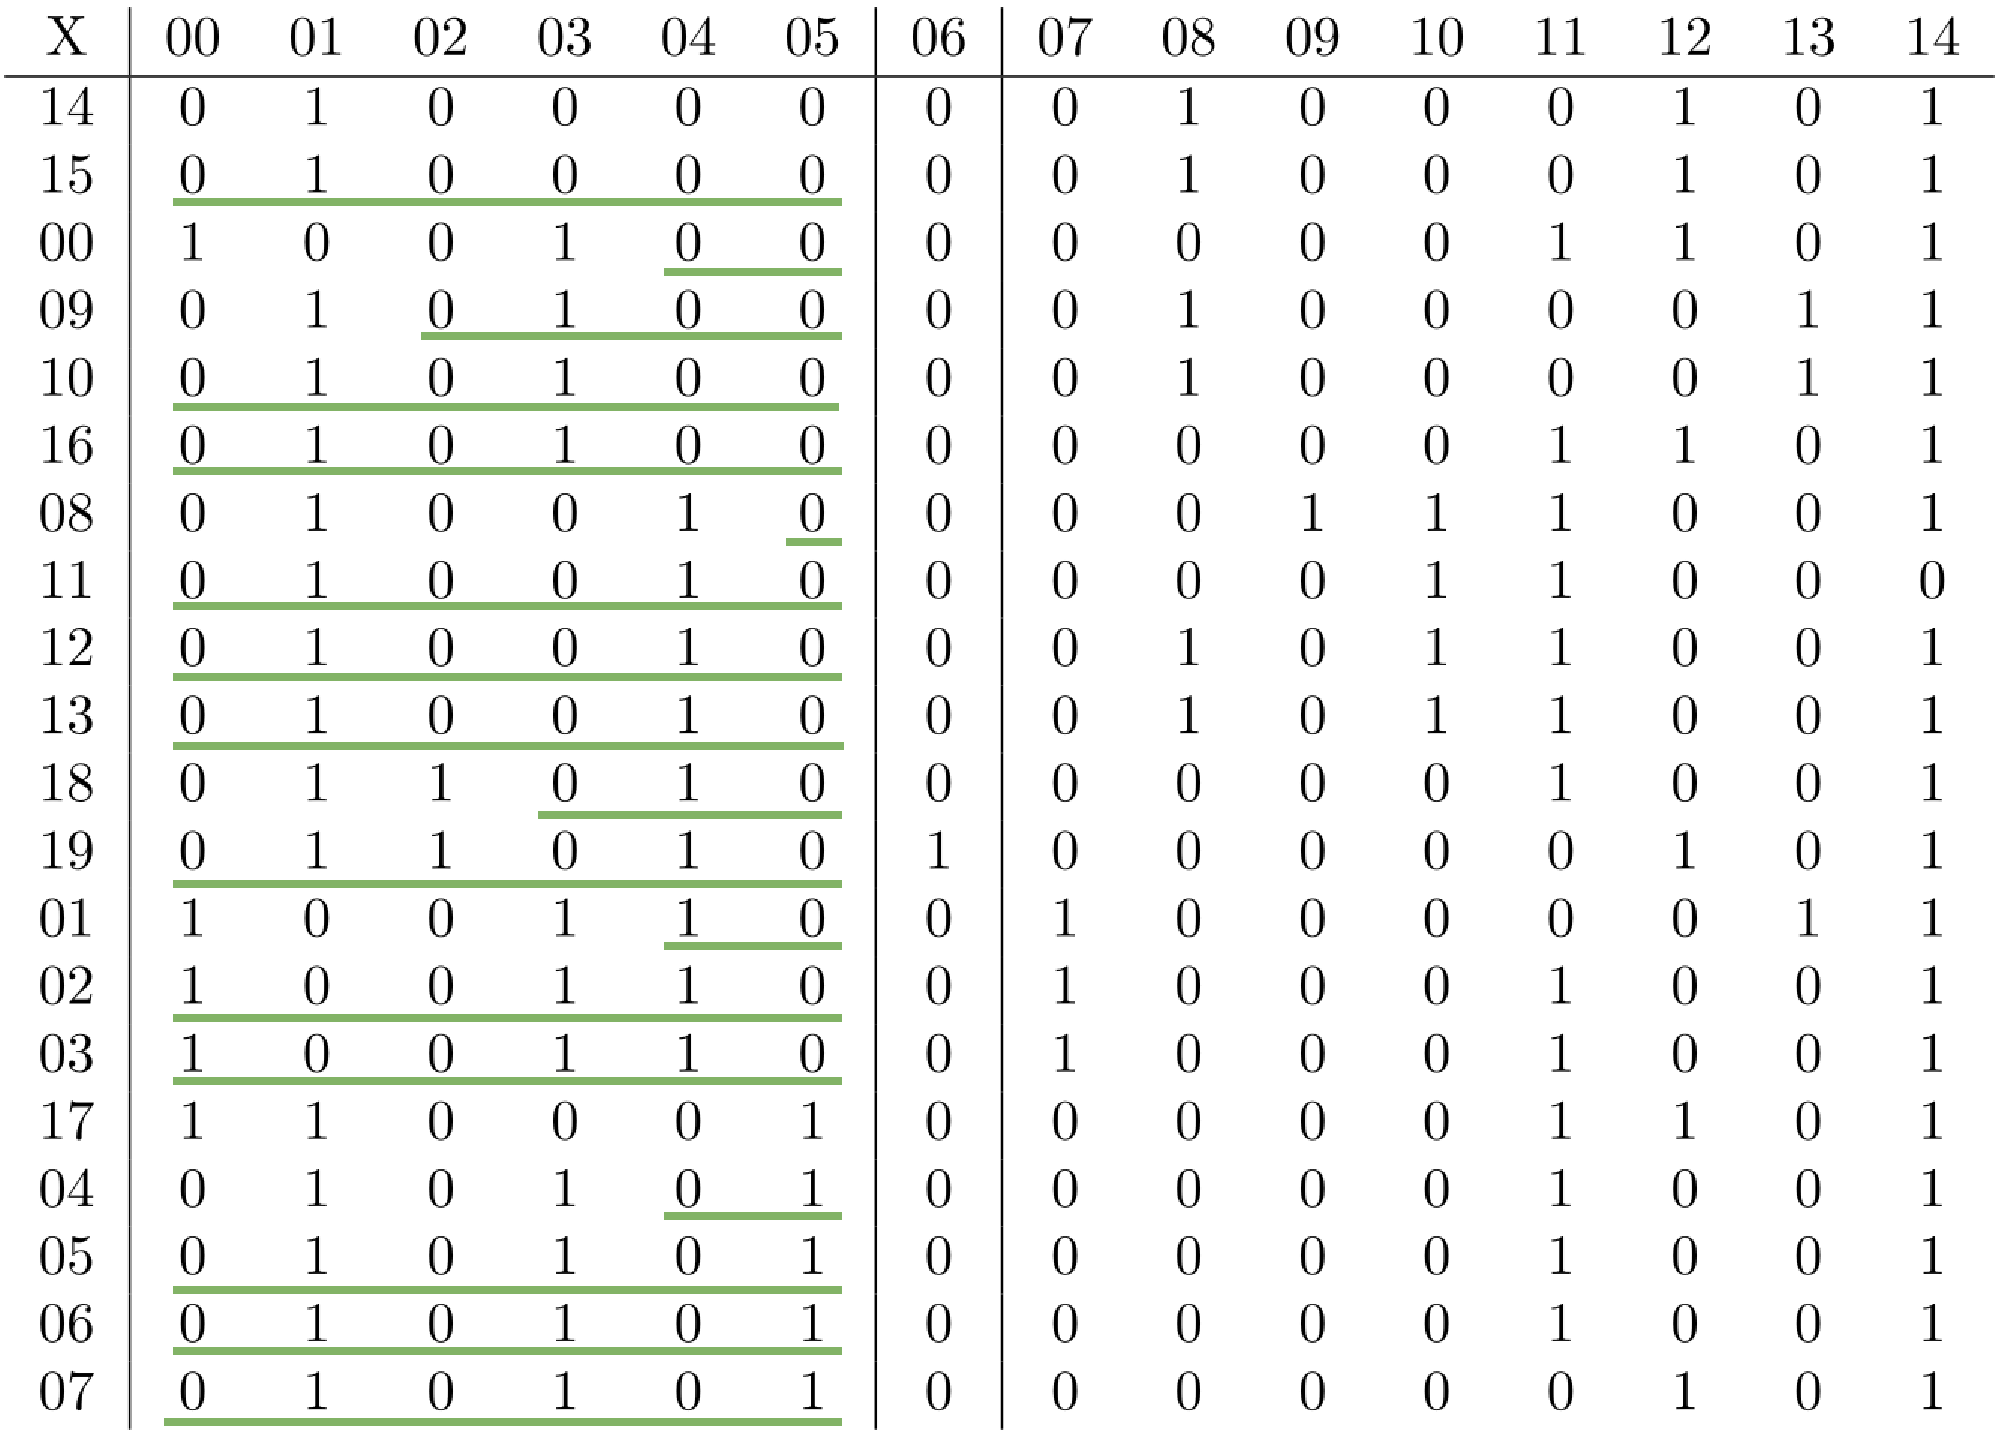
\includegraphics[scale = 0.365]{img/matrix1.pdf}
  \end{figure}
  Ottenendo quindi:
  \[a_6=[14,15,0,9,10,16,8,11,12,13,18,19,1,2,3,17,4,5,6,7]\]
  \[\alpha_6=[2,12,13,14,16,17,18,19,6,3,4,7,8,9,0,1,5,15,10,11]\]
  \[d_6=[6,0,4,2,0,0,5,0,0,0,3,0,4,0,0,6,4,0,0,0]\]
  \[l_6=[0,6,2,4,6,6,1,6,6,6,3,6,2,6,6,0,2,6,6,6]\]
  Nel complesso, permutando con tutti i vari \textit{prefix array}, si
  otterrebbe la seguente \textbf{matrice PBTW}:
  \begin{table}[H]
  \centering
  \footnotesize
  \begin{tabular}{c|ccccccccccccccc}
    X & 00 & 01 & 02 & 03 & 04 & 05 & 06 & 07 & 08 & 09 & 10 & 11 & 12 & 13
    & 14 \\
    \hline
    00 & 1 & 1 & 0 & 1 & 1 & 0 & 0 & 0 & 1 & 0 & 0 & 1 & 1 & 1 & 1 \\
    01 & 1 & 1 & 0 & 1 & 1 & 0 & 0 & 0 & 1 & 0 & 0 & 1 & 1 & 1 & 1 \\
    02 & 1 & 1 & 0 & 1 & 1 & 1 & 0 & 0 & 0 & 1 & 1 & 1 & 0 & 1 & 1 \\
    03 & 1 & 1 & 0 & 1 & 1 & 0 & 0 & 0 & 1 & 0 & 0 & 1 & 1 & 0 & 1 \\
    04 & 0 & 1 & 0 & 1 & 0 & 1 & 0 & 0 & 1 & 0 & 0 & 1 & 1 & 0 & 1 \\
    05 & 0 & 1 & 0 & 1 & 0 & 1 & 0 & 0 & 0 & 0 & 0 & 1 & 0 & 0 & 1 \\
    06 & 0 & 1 & 0 & 1 & 0 & 1 & 0 & 0 & 0 & 0 & 0 & 1 & 0 & 0 & 0 \\
    07 & 0 & 1 & 0 & 1 & 1 & 1 & 0 & 0 & 0 & 0 & 0 & 0 & 1 & 0 & 1 \\
    08 & 0 & 1 & 0 & 0 & 1 & 0 & 0 & 0 & 1 & 0 & 0 & 0 & 1 & 0 & 1 \\
    09 & 0 & 1 & 0 & 1 & 0 & 0 & 0 & 0 & 1 & 0 & 0 & 0 & 0 & 0 & 1 \\
    10 & 0 & 1 & 0 & 1 & 1 & 0 & 0 & 0 & 0 & 0 & 0 & 1 & 1 & 0 & 1 \\
    11 & 0 & 1 & 0 & 0 & 1 & 0 & 1 & 1 & 0 & 0 & 0 & 1 & 0 & 0 & 1 \\
    12 & 0 & 1 & 0 & 0 & 1 & 0 & 0 & 1 & 0 & 0 & 0 & 0 & 0 & 0 & 1 \\
    13 & 0 & 1 & 0 & 0 & 0 & 0 & 0 & 1 & 0 & 0 & 0 & 0 & 0 & 0 & 1 \\
    14 & 0 & 1 & 0 & 0 & 0 & 0 & 0 & 0 & 0 & 0 & 0 & 0 & 0 & 0 & 1 \\
    15 & 0 & 0 & 0 & 0 & 0 & 0 & 0 & 0 & 0 & 0 & 0 & 0 & 0 & 0 & 1 \\
    16 & 0 & 0 & 0 & 1 & 0 & 0 & 0 & 0 & 0 & 0 & 0 & 1 & 0 & 0 & 1 \\
    17 & 1 & 0 & 1 & 0 & 0 & 0 & 0 & 0 & 0 & 0 & 1 & 1 & 0 & 0 & 1 \\
    18 & 0 & 0 & 1 & 0 & 0 & 0 & 0 & 0 & 0 & 0 & 1 & 1 & 0 & 0 & 1 \\ 
    19 & 0 & 1 & 0 & 0 & 0 & 0 & 0 & 0 & 0 & 0 & 1 & 1 & 0 & 0 & 1
  \end{tabular}
\end{table}
\end{esempio}
\subsection{Match con aplotipo esterno}
Durbin, nel suo articolo, propone diversi algoritmi, ad esempio per il calcolo
di match interni ad $X$ più lunghi di una lunghezza minima $L$ o per la ricerca
di tutti i \textit{set-maximal match} interni ad $X$ in tempo lineare. Di
interesse per questa tesi è però il cosiddetto \textit{algoritmo 5}, quello che
si propone di trovare tutti i \textit{set-maximal match} tra il panello $X$ e un
aplotipo esterno $z$, assumendo che $|z|=M$.\\
L'idea dietro l'algoritmo è quella di usare tre indici: $e_k$, $f_k$ e
$g_k$. Nel dettaglio $e_k$ tiene traccia dell'inizio del più lungo match,
terminante in colonna $k$, tra $z$ e un qualche $y_i^k$. L'intervallo
$[f_k,g_k)\subseteq[0,\ldots,M)$ invece identifica il sotto-intervallo di
$a_k$ contenente gli indici degli aplotipi appartenetenti a tale match.
Formalmente si ha quindi che:
\[z[e_k,k)=y_i^k[e_k,k)\land z[e_k-1]\neq y_i^k[e_k-1], \forall i\mbox{
    t.c. }f_k\leq i < g_k\]
Si noti che $g_k=M$ sse $y_{M-1}^k$ appartiene alle sequenze per cui si ha tale
match più lungo.\\
Bisogna quindi capire come aggiornare $e_k$, $f_k$ e $g_k$ passando dalla
colonna $k$ alla colonna $k+1$. L'idea è quella per cui, avendo
$f_{k+1}<g_{k+1}$ allora sicuramente ho ancora delle righe che presentano un
match che parte da $e_k=e_{k+1}$ e termina in $k$ che può essere esteso in
$k+1$. In caso contrario, avendo $f_{k+1}=g_{k+1}$, non si hanno match
estendibili e quindi si può concludere che quelli terminanti in colonna $k$
erano match massimali, dovendo poi aggiornare $e_{k+1}$ ottenedo i relativi
$f_{k+1}$ e $g_{k+1}$. Bisogna quindi capire come funzioni la
variante dell'\textbf{LF-mapping}, guidato dal carattere corrente dell'aplotipo
query, all'interno della \textbf{PBWT}, per ottenere $f_{k+1}$ e $g_{k+1}$ a
partire da $f_k$ e $g_k$ (e di conseguenza $e_{k+1}$).\\ 
Per effettuare il mapping abbiamo bisogno di tre componenti:
\begin{enumerate}
  \item l'array $c$ tale per cui $c[k]=j$ sse la colonna $k$ contiene $j$
  occorrenze di 0
  \item l'array $u_k$ tale per cui, alla colonna $k$-esima, $u_k[i]=j$ sse $j$ è
  il numero di occorrenze di 0 prima dell'indice $i$ nella colonna $k$
  \item l'array $v_k$ tale per cui, alla colonna $k$-esima, $v_k[i]=j$ sse $j$ è
  il numero di occorrenze di 1 prima dell'indice $i$ nella colonna $k$ 
\end{enumerate}
Tali valori possono essere computati e memorizzati in fase di costruzione della
\textbf{PBWT}, come visibile direttamente nell'algoritmo \ref{algo:durbin1} per
quanto riguarda $u$ e $v$, avendone già la computazione. Per quanto riguarda $c$
si ha che potrebbe essere banalmente calcolato anch'esso in fase di costruzione
della \textbf{PBWT}, tenendo ogni volta traccia del numero di 0 incontrati
nella colonna $k$-esima.\\
Sfruttando i valori di questi 3 array possiamo quindi effettuare il mapping,
definito per comodità da una funzione, rappresentabile in pseudocodice come
nell'algoritmo \ref{algo:lf}:
\[w_k:\{0,\ldots,N\}\times\Sigma\to \{0,\ldots,N\}\]
tale per cui:
\[w_k(i,\sigma)=
  \begin{cases}
    u_k[i]&\mbox{ se }\sigma=0\\
    v_k[i]+c[k]&\mbox{ se }\sigma=1
  \end{cases}
\]
Infatti, come confermato anche dall'algoritmo di costruzione stesso, si ha che:
\[a_{k+1}\left[w_k\left(i,y_i^k[k]\right)\right]=a_k[i]\]
\begin{esempio}
  Vediamo un piccolo esempio chiarificatore, riprendendo il precedente.\\
  Per praticità riporta che:
  \[a_5=[14,15,17,0,4,5,6,7,9,10,16,8,11,12,13,18,19,1,2,3]\]
  \[\alpha_5=[3,17,18,19,4,5,6,7,11,8,9,12,13,14,0,1,10,2,15,16]\]
  \[a_6=[14,15,0,9,10,16,8,11,12,13,18,19,1,2,3,17,4,5,6,7]\]
  \[\alpha_6=[2,12,13,14,16,17,18,19,6,3,4,7,8,9,0,1,5,15,10,11]\]
  Si ha quindi, ad esempio, con $k=5$ e $i=2$, che:
  \[a_{6}\left[w_5\left(2,y_2^5[5]\right)\right]=a_5[2]\]
  Avendo:
  \[w_5\left(2,y_2^5[5]\right)=w_5\left(2,1\right)=v_5[2]+c[5]=0+15=15\]
  Si ha che:
  \[a_{6}[15]=17=a_5[2]\]
\end{esempio}
Ai fini dell'algoritmo serve però il ``passaggio inverso'' rispetto a quello
indicato da questa equazione, ovvero passare dalla colonna $k$ alla colonna
$k+1$. Quindi, pensando alla permutazione inversa del \textbf{prefix array}, si
ha che:
\[\alpha_{k+1}[i]=w_k(\alpha_k[i],x_i[k])\]
\begin{esempio}
  Si riprendono i dati dell'esempio precedente e si vuole calcolare, sempre con
  $k=5$ e $i=2$:
  \[\alpha_{6}[2]=w_5(\alpha_5[2],x_2[5])=w_5(18,0)=13\]
  Come volevasi dimostrare.
\end{esempio}
L'ultima equazione ci suggerisce quindi che l'LF-mapping sopra definito
consente il corretto aggiornamento di $f_k$ e $g_k$.
Definendo quindi:
\[f_{k+1}=w_k(f,z[k])\]
si ha che $f_{k+1}$ sarà l'indice, in $a_{k+1}$, della prima sequenza $y_j^k$,
con $j\geq f$, per la quale $y_j^k[k]=z[k]$. Analogamente si ha anche:
\[g_{k+1}=w_k(g,z[k])\]
Si hanno quindi, dopo il calcolo di $f_{k+1}$ e $g_{k+1}$ due possibili casi:
\begin{enumerate}
  \item si ha che $f_{k+1}<g_{k+1}$, quindi si hanno ancora match che partono da
  $e_k$ e terminano in $k$ che si estendono anche in $k+1$. In tal caso quindi
  $e_{k+1}=e_k$
  \item si ha che $f_{k+1}=g_{k+1}$, quindi non si hanno match che partono da
  $e_k$ e terminano in $k$ che sono anche estendibili in $k+1$. Bisogna quindi
  annotare i match terminanti in $k$, nell'intervallo $[f_k,g_k)$ su $a_k$,
  e poi calcolare i nuovi $e_k$, $f_k$ e $g_k$. La chiave per questo calcolo è
  che, virtualmente, l'aplotipo $z$ si trova o  subito prima del blocco di
  aplotipi $[f_k,g_k)$ in colonna $k$, secondo l'ordinamento dato dalla medesima
  colonna, o subito dopo. Si ha quindi che, essendo nell'ordinamento o subito
  prima di $f_{k}$ o subito dopo $g_k$:
  \[y_{f_{k+1}-1}^{k+1}<z<y_{f_{k+1}}^{k+1}\]
  Diventa quindi possibile inferire che:
  \[e_{k+1}\leq d_{k+1}[f_{k+1}]\]
  Si considera quindi, come punto di partenza $e_{k+1}=d_{k+1}[f_{k+1}]-1$,
  studiando di conseguenza $z[e_{k+1}]$, avendo due casi possibili:
  \begin{enumerate}
    \item se tale valore è 0 allora, per l'ordinamento, $z$ ha un match migliore
    con $y_{f_{k+1}-1}^{k+1}$ rispetto che con $y_{f_{k+1}}^{k+1}$. Si aggiorna
    quindi $e_{k+1}$, decrementandolo, fino a che si ha match tra $z[e_{k+1}-1]$
    e $y_{f_{k+1}-1}^{k+1}[e_{k+1}-1]$. Infine si decrementa $f_{k+1}$ fino a
    che $d_{k+1}[f_{k+1}]\leq e_{k+1}$, trovando quelle righe per il quale il
    \textbf{divergence array} non supera il valore di $e_{k+1}$. Si ottengono in
    tal modo le sequenze, nel riordinamento in $k+1$, che hanno un match da
    $e_{k+1}$ a $k+1$. Invece $g_{k+1}$ resta fisso
    \item se tale valore è 1 allora, per l'ordinamento, $z$ ha un match migliore
    con $y_{f_{k+1}}^{k+1}$ rispetto che con $y_{f_{k+1}-1}^{k+1}$. Si aggiorna
    quindi $e_{k+1}$, decrementandolo, fino a che si ha match tra $z[e_{k+1}-1]$
    e $y_{f_{k+1}-1}^{k+1}[e_{k+1}-1]$. Infine si incrementa $g_{k+1}$ fino a
    che $d_{k+1}[g_{k+1}]\leq e_{k+1}$, per lo stesso ragionamento del caso
    precedente. Invece $f_{k+1}$ resta fisso 
  \end{enumerate}
\end{enumerate}
\textbf{METTERE ESEMPIO}\\
L'algoritmo 5 è visualizzabile all'algoritmo \ref{algo:dur5} e, secondo i
calcoli di Durbin, ha complessità $\mathcal{O}(NM)$, in quanto si ritiene che il
numero di accessi ai loop interni sia limitato dalla costante rappresentante il
numero di match, $c$. Nonostante ciò tale complessità temporale è ancora in
corso di studio in quanto si hanno in letteratura evidenze della sua non
correttezza. Un esempio è il paper di Naseri \cite{dpbwt}, dove si afferma che
l'intuizione per cui tale costante $c$ limiti superiormente gli accessi ai loop
innestati sia falsa. Si noti che nell'articolo non viene però precisata una
nuova misura per la complessità dell'algoritmo.
\textbf{VERIFICARE ULTIMA FRASE (MA ANCHE TUTTO IL RESTO CHE VA SCRITTO MEGLIO)}
\begin{algorithm}
  \begin{algorithmic}   
    \Function{Find\_Set\_Maximal\_Matches\_From\_Z}{$z$}
    \For {$k\gets 0$ \textbf{to} $N$}
    \State $e,f,g\gets \mbox{\textit{Update\_Z\_Matches}}(k, z, e, f, g)$
    \EndFor
    \EndFunction    
    \Function{Update\_Z\_Matches}{$k, z, e, f, g$}
    \State $f'\gets w(k, f, z[k])$
    \State $g'\gets w(k, g, z[k])$
    \If{$f'<g'$}
    \Comment\textit{{se $k$ è $N-1$ match da $e_k$ a $N-1$}}
    \State $e'\gets e_k$
    \Else
    \Comment{\textit{match da $e_k$ a $k$}}
    \State $e'\gets d_{k+1}[f']-1$
    \If{$z[e']=0$ \textbf{and} $f'>0$}
    \State $f'\gets g'-1$
    \State \textbf{while} $z[e'-1]=y_{f'}^{k+1}[e'-1]$ \textbf{do} $e'\gets
    e'-1$
    \State \textbf{while} $d_{k+1}[f']\leq e'$ \textbf{do} $f'\gets f'-1$
    \Else
    \State $g'\gets f'+1$
    \State \textbf{while} $z[e'-1]=y_{f'}^{k+1}[e'-1]$ \textbf{do}  $e'\gets
    e'-1$ 
    \State \textbf{while} $g'<M$ \textbf{and} $d_{k+1}[g']\leq e'$ \textbf{do}
    $g'\gets g'+1$ 
    \EndIf
    \EndIf
    \State \textbf{return} $e',f',g'$
    \EndFunction
  \end{algorithmic}
  \caption{Algoritmo 5 di Durbin.}
  \label{algo:dur5}
\end{algorithm}
\subsubsection{Limiti spaziali}
Bisogna affrontare la tematica della complessità in spazio di tale
algoritmo. Ipotizzando di non ricalcolare colonna per colonna tutti i dati
necessari (comportando un'incremento dal punto di vista temporale).\\
Ricapitolando, per poter eseguire l'algoritmo 5, si necessita di avere in
memoria, con \textit{random access} in tempo costante:
\begin{itemize}
  \item il \textbf{pannello} $X$, di dimensione $NM$
  \item il \textbf{prefix array} $a_k$, di dimensione $NM$
  \item il \textbf{divergence array} $d_k$, di dimensione $NM$
  \item i vettori $u_k$ e $v_k$, complessivamente di dimensione $2NM$
  \item il vettore $c_k$, di dimensione $M$
\end{itemize}
Possiamo quindi dire che si ha una complessità in memoria pari a
$\mathcal{O}(NM)$ e, nel dettaglio, Durbin stima si tratti di $13NM$
byte\footnote{\url{https://github.com/richarddurbin/pbwt/blob/0de8d02df1b77146ded81e9e196991fdab520767/pbwtMatch.c#L252}}.\\
Per poter capire meglio la problematica prendiamo ad esempio un pannello di
medie dimensioni, con $N=30000$ e $M=100000$. Ne segue che, secondo la stima di
Durbin, si necessitano $\sim 36.32$ gigabytes di memoria. Inoltre, una stima
sperimentale di tale richiesta di memoria può essere confermata con l'esecuzione
dell'implementazione della \textbf{PBWT} di Durbin stesso. Infatti, monitorando
con \texttt{time} il picco di memoria durante l'esecuzione si ha che esso
corrisponde a $\sim 40.76$ gigabytes (comprensivi anche di tutto ciò che è ``a
contorno'' all'algoritmo stesso). I dati quindi sembrano confermare le stime di
Durbin e confermano l'alto uso di memoria richiesto dall'algoritmo 5. Questa è
stata la motivazione principale per cui si è sviluppata, in questa tesi
magistrale, una versione \textbf{run-length encoded} della struttura dati che
permettesse di effettuare query con un aplotipo esterno
\subsection{Varianti della PBWT}
\subsubsection{PBWT multi-allelica}
\subsubsection{PBWT con struttura LEAP}
\subsubsection{PBWT dinamica}
\subsubsection{PBWT bidirezionale}
%\subsubsection{Recenti sviluppi}
% LocalWords:  pseudocodice



\chapter{Metodo}
\label{metchap}
In questo capitolo verranno illustrate le metodologie usate in questa tesi,
trattando, sia dal punto di vista teorico che sperimentale, tutte le soluzioni
che hanno portato alla costruzione della \textbf{RLPBWT}.\\
Nel dettaglio, si approfondiranno tutte le varianti della \textbf{RLPBWT}
ottenute durante lo studio, evidenziandone pro e contro.

% sezione varianti RLPBWT
\section{Perché la compressione run-length}
Prima di proseguire con la spiegazione dettagliata delle varianti della
$\RLPBWT$, è bene dare 
un'ulteriore motivazione al perché si sia ritenuto utile sviluppare una variante
run-length encoded della $\PBWT$.\\
Una motivazione la si ha citando direttamente il paper di Durbin sulla
$\PBWT$ \cite{pbwt}: 
\begin{center}
  \textit{Furthermore we can also expect the $y$ arrays to be strongly
    run-length compressible. This is because population genetic structure means
    that there 
    is local correlation in values due to linkage disequilibrium, which means
    that haplotypes with similar prefixes in the sort order will tend to have
    the same allele values at the next position, giving rise to long runs of
    identical values in the $y$ array. So the $\PBWT$ can easily be stored in
    smaller space than the original data.} 
\end{center}
Quindi, il risultato atteso è quello per cui aplotipi simili, che, ad ogni step,
saranno consecutivi nel riordinamento inverso, è molto probabile presentino lo
stesso 
allele nella colonna di cui si sta calcolando la
permutazione. Ne segue che, all'interno della matrice $\PBWT$, è molto
probabile che si abbiano lunghe run di simboli $\sigma=0$ e di simboli
$\sigma=1$.
Si ottiene il medesimo risultato atteso avuto con
la $\BWT$, dove si aveva che caratteri uguali era molto probabile fossero posti
in posizioni consecutive all'interno della trasformata stessa. Si hanno, di
conseguenza, le
stesse premesse che hanno portato alla $\RLBWT$, considerando, inoltre,
che non si tratta solo di memorizzare la struttura con
compressione run-length ma di lavorare direttamente con la struttura dati
compressa, risolvendo il problema del calcolo degli $\SMEM$ senza
decomprimere la struttura dati. Ipotizzando che, per una certa colonna della
matrice $\PBWT$, il numero di run sia molto minore della lunghezza della
colonna stessa, si deduce facilmente che l'uso della compressione run-length
possa comportare una riduzione significativa della memoria necessaria all'uso
della trasformata.
\section{Matching Statistics per la RLPBWT}
Bisogna, per prima cosa, introdurre il 
concetto di \textbf{matching statistics} nel caso della $\PBWT$ (e quindi
anche della sua variante run-length encoded).
\begin{definizione}
  Dato un pannello $X$, con $M$ individui aventi $N$ siti,
  e un aplotipo esterno/pattern $z$, tale che $|z|=N$, si definisce matching
  statistics di $z$ su $X$ un array $\MS$ di coppie $(\row,\len)$, di lunghezza
  $N$, tale che (avendo che $x_i$ indica l'$i$-esima riga del pannello $X$): 
  \begin{itemize}
    \item $x_{\MS[i].\row}[i-\MS[i].\len+1,i]=z[i-\MS[i].\len+1,i]$, ovvero si
    ha che 
    l'aplotipo esterno ha un match, lungo $\MS[i].\len$, terminante in colonna
    $i$, con la riga 
    $\MS[i].\row$-esima del pannello
    \item $z[i-\MS[i].\len,i]$ non è un suffisso terminante in colonna $i$ di un
    qualsiasi sottoinsieme di righe di $X$. In altri termini, il match non deve
    essere ulteriormente estendibile a sinistra
  \end{itemize}
\end{definizione}
\noindent
Analogamente al caso della variante classica, si ha il seguente lemma.
\begin{lemma}
  Dato un pannello $X$, di dimensioni $M\times N$, con $M$ individui e $N$
  siti, un aplotipo esterno/pattern $z$, tale che $|z|=N$, e il corrispondente
  array di matching statistics $\MS$ si ha che $z[i-l+1,i]$
  presenta uno $\SMEM$ di lunghezza $l$ con la riga $\MS[i].\row$-esima del
  pannello $X$ sse: 
  \begin{equation}
    \label{eq:rlpbwtsmem}
    \MS[i].\len=l\land(i=N-1\lor \MS[i].\len\geq \MS[i+1].\len)
  \end{equation}
\end{lemma}
\noindent
\textit{Si vedrà in sezione \ref{secphi} come calcolare, a partire da tali
  $\SMEM$, tutte le righe del panello per le quali si ha il medesimo
  $\SMEM$}.\\
Il calcolo dell'array $\MS$ di $z$ rispetto al pannello $X$ si basa su due fasi:
\begin{enumerate}
  \item la fase di \textbf{start}
  \item la fase di \textbf{extend}
\end{enumerate}
Si assuma di avere due indici $i$ e $j$, $0\leq i\leq j< N$, tali per cui
$z[i,j]$ è un suffisso di uno tra $x_0[0,j]$, \ldots, $x_{M-1}[0,j]$. \\
La fase di extend estende il match di $z[i,j]$ a $z[i,j+1]$ sse:
\begin{itemize}
  \item $j<N$
  \item $z[i,j+1]$ è un suffisso di uno tra $x_0[0,j+1]$, $\ldots$,
  $x_{M-1}[0,j+1]$ 
\end{itemize}
La fase di start cerca il più piccolo indice $i'$,
avendo $i\leq i'\leq j$, tale per cui $z[i',j]$ è un suffisso di uno tra
$x_0[0,j]$, $\ldots$, $x_{M-1}[0,j]$.\\
Si ha quindi il computo di ogni coppia di valori $\MS[i]$, $\forall i\in[0,N)$:
\begin{itemize}
  \item si assume inizialmente che $\MS[0].\len=0$, quando $i=0$
  \item si applica la fase di start per cercare il minimo indice
  $i'$, avendo $i\leq i'$, tale che $z[i',i'+\MS[i].\len]$ è un suffisso di uno
  tra $x_0[0,i'+\MS[i].\len], \ldots$ $x_{M-1}[0,i'+\MS[i].\len]$. Inoltre, per
  minimalità di $i'$, si ha che, $\forall i<j<i'$,
  $\MS[j].\len=\MS[j-1].\len-1$, $\forall j\in[i+1,i'-1]$
  \item si itera la fase di extend per trovare il
  più lungo prefisso $z[i',k]$ che è anche un suffisso di uno tra $x_0[0,k]$,
  $\ldots$, $x_{M-1}[0,k]$, avendo che $\MS[i'].\len=k-i'+1$
  \item avendo che $i'>i$, si può procedere induttivamente al calcolo dell'array
  $\MS$ 
\end{itemize}
Per convenzione, si ha che, nella prima colonna, l'iterazione parte dall'ultima
riga. Tale scelta è, in ogni caso, arbitraria. 
In modo
analogo, qualora si abbia una colonna $k$ di un solo carattere, non
corrispondente a quello della query, si sceglie l'ultima riga della
colonna successiva, dalla quale si riprende il calcolo  
dell'array delle matching statistics, dopo aver memorizzato $\MS[k].\row=M$
(un valore sentinella non esistendo la riga di indice $M$) e $\MS.\len[k]=0$.\\
In altri termini, più ``pratici'', il calcolo dell'array $\MS$ avviene nel
seguente modo:
\begin{itemize}
  \item si parte da una riga arbitraria $i$ della prima colonna
  \item se si ha $x_i[0]=z[0]$, si procede salvando $\MS[0].\row=i$
  \item qualora si abbia $x_i[0]\neq z[0]$, si seleziona o l'ultima riga della
  run precedente o la prima riga della run successiva a quella a cui appartiene
  la riga $i$. Tale riga verrà salvata come $\MS[0].\row=j$ e da essa si
  proseguirà l'esecuzione dell'algoritmo
  \item si effettua il mapping verso la colonna successiva, $k$,
  e, a seconda di avere o meno un match con $z[k]$, si procede come nei casi
  visti sopra 
\end{itemize}
Si noti che non si è parlato di come calcolare i valori $\MS[i].\len$, in
quanto si hanno due soluzioni (approfondite in seguito), che
rispecchiano quanto visto con 
MONI \cite{moni} e PHONI \cite{phoni} per la $\RLBWT$: 
\begin{enumerate}
  \item si possono usare le threshold, per capire quale nuova riga
  selezionare in 
  caso di mismatch. In tal caso, i valori $\MS[i].\len$ devono essere calcolati
  successivamente al calcolo dei valori $\MS[i].\row$, tramite random
    access al panello
  \item si possono usare le $\LCE$ query, per capire quale nuova riga
  selezionare in caso di mismatch. In tal caso, il calcolo dei valori
  $\MS[i].\len$ avviene in contemporanea al calcolo dei valori $\MS[i].\row$
\end{enumerate}
\begin{esempio}
  \label{es:ms}
  Si riprenda, al fine di vedere un esempio di calcolo dell'array $\MS$,
  l'esempio \ref{es:algo5}, con i seguenti $\SMEM$ tra la query $z$ e il
  pannello $X$:
  \begin{figure}[H]
    \centering
    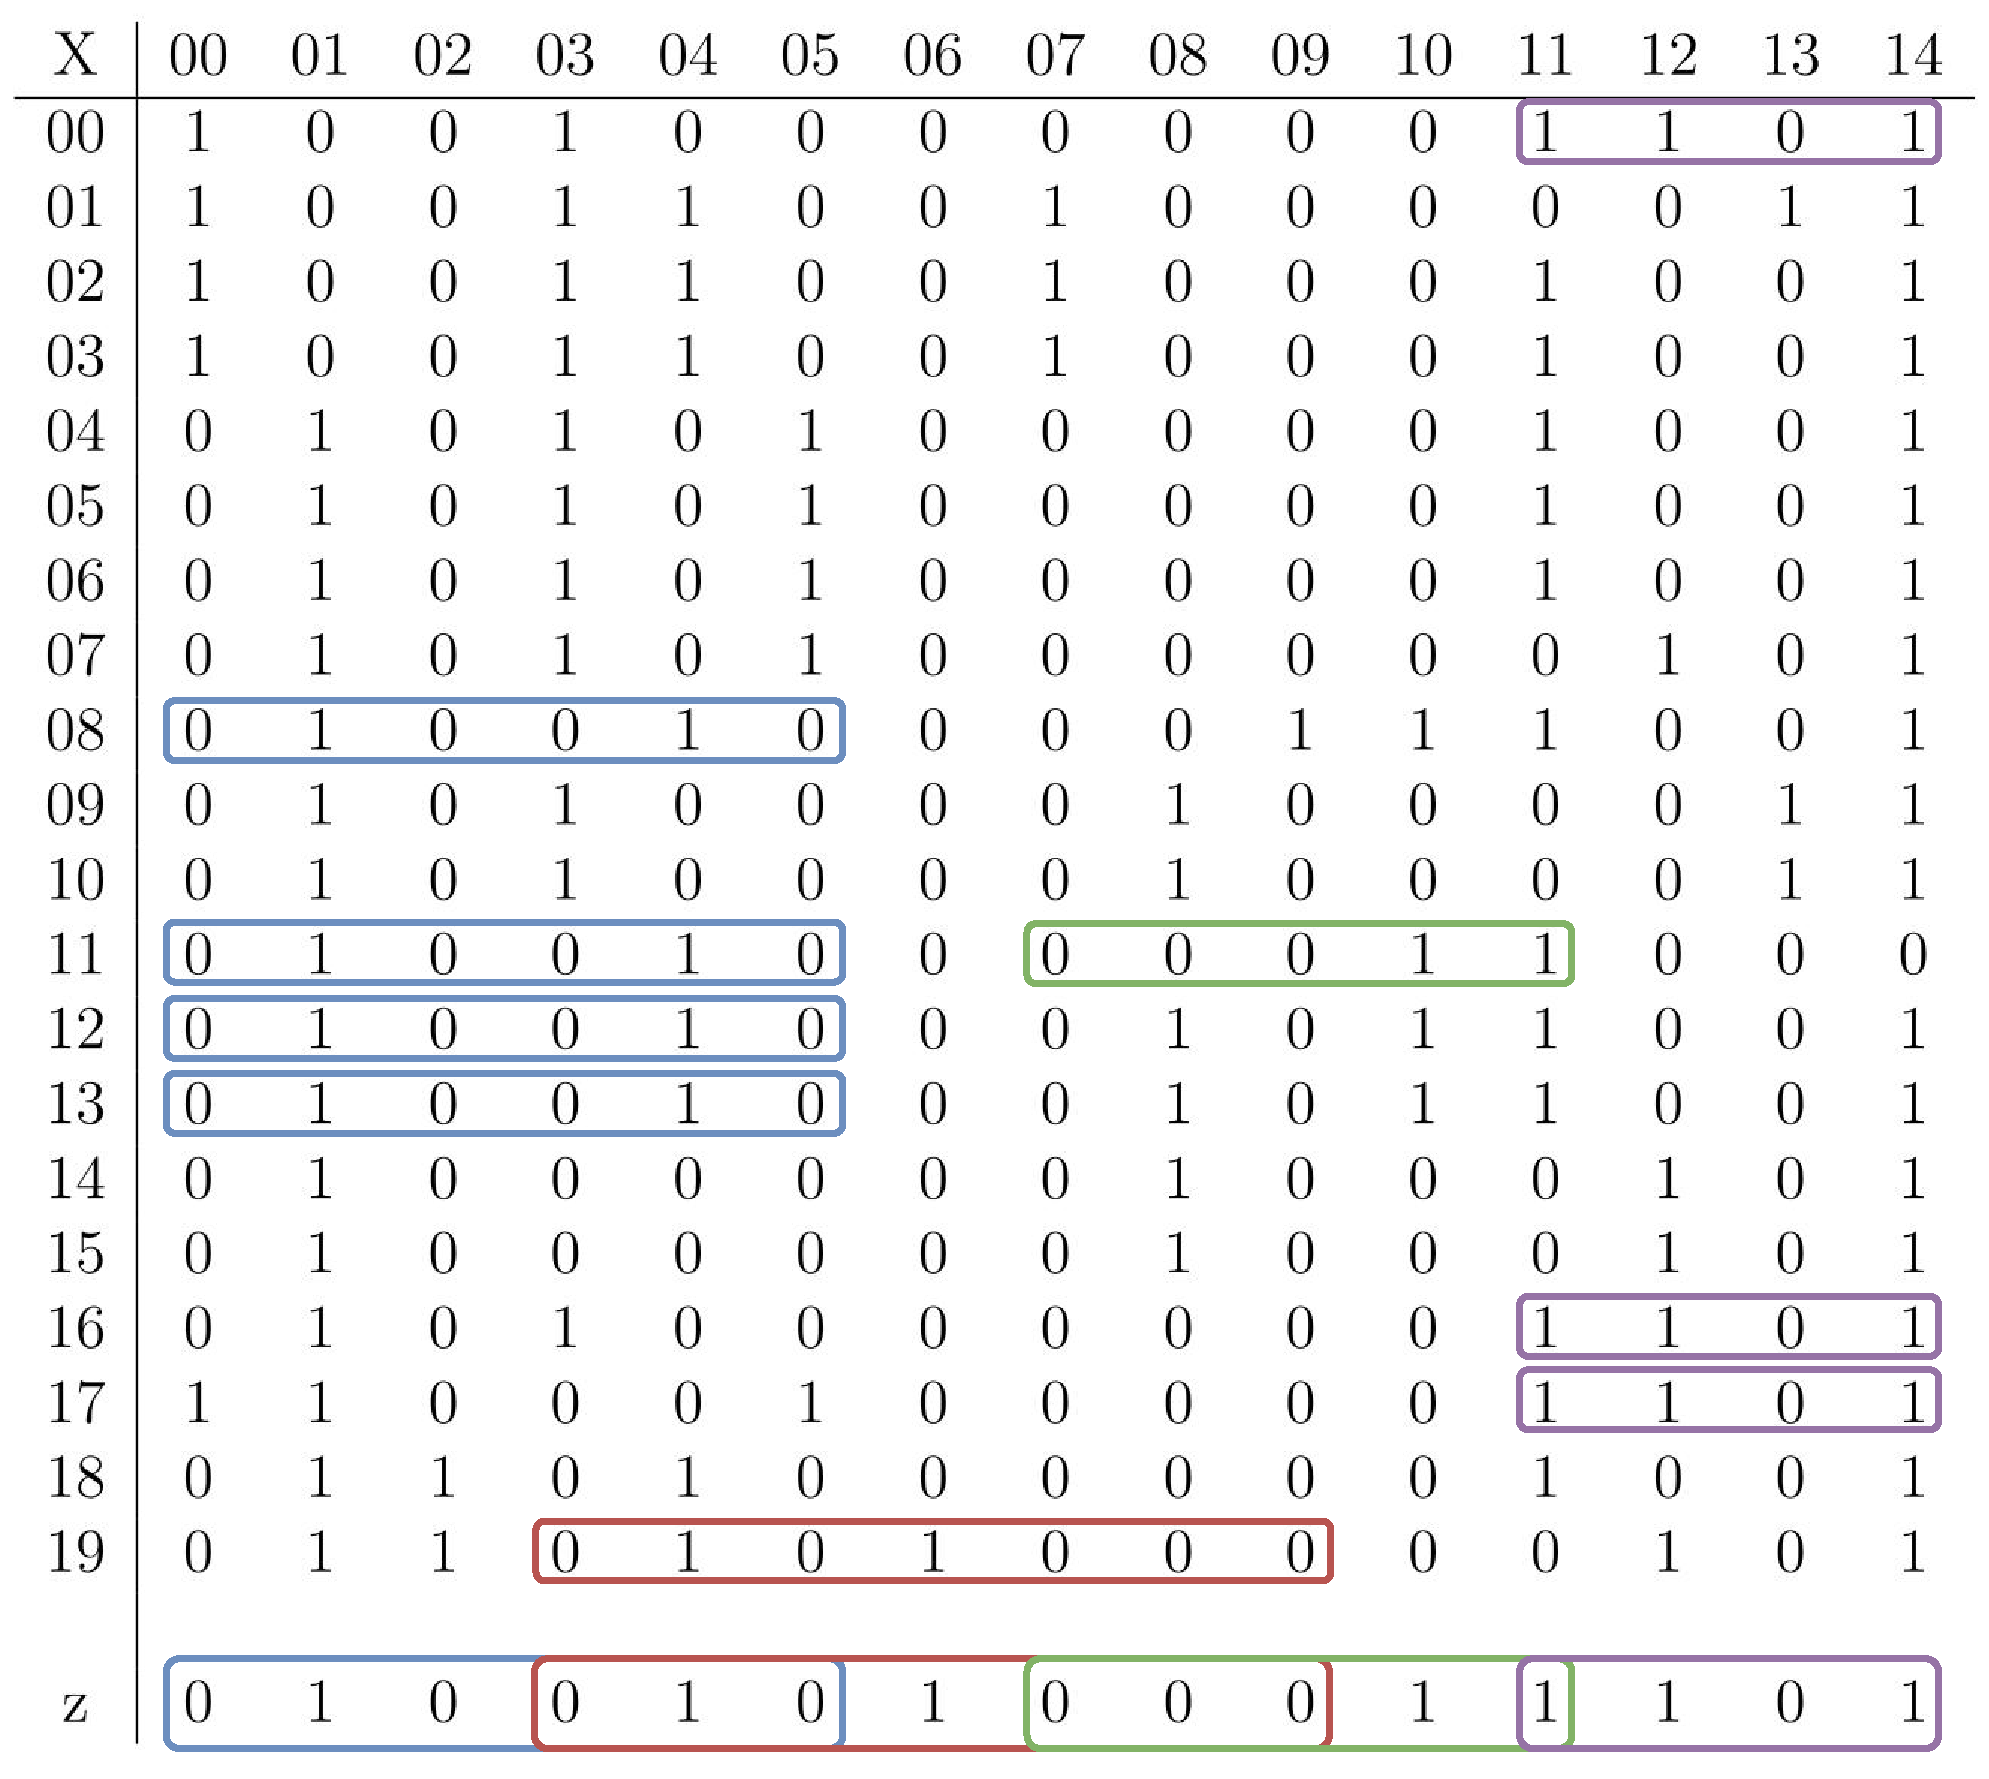
\includegraphics[scale = 0.345]{img/pbwtmatch.pdf}
  \end{figure}
  In tal caso l'array $\MS$ sarebbe, iniziando il computo dalla riga 19:
  \begin{table}[H]
    \footnotesize
    \centering
    \begin{tabular}{c|ccccccccccccccc}
      $k$ & 00 & 01 & 02 & 03 & 04 &  {\color{nordcyan}05} & 06 & 07 & 08
      &  {\color{nordred}09} & 10 &  {\color{nordgreen}11} & 12 & 13
      &  {\color{nordpurple}14} \\
      \hline
      \hline
      $z$ & 0 & 1 & 0 & 0 & 1 &  {\color{nordcyan}0} & 1 & 0 & 0
      &  {\color{nordred}0} & 1 &  {\color{nordgreen}1} & 1 & 0
      &  {\color{nordpurple}1} \\
      \hline
      $\row$ & 19 & 19 & 16 & 15 & 13 &  {\color{nordcyan}13} & 19 & 19 & 19
      &  {\color{nordred}19} & 11 &  {\color{nordgreen}11} & 17 & 17
      &  {\color{nordpurple}17} \\
      $\len$ & 1 & 2 & 3 & 4 & 5 & {\color{nordcyan}6} & 4 & 5 & 6
      & {\color{nordred}7} & 4 & {\color{nordgreen}5} & 2 & 3
      & {\color{nordpurple}4}\\
    \end{tabular}
  \end{table}
  In $\MS$ si possono riconoscere i vari $\SMEM$, la cui colonna di fine è
  segnalata nello stesso colore con cui si rappresentano gli $\SMEM$ nel
  pannello. 
\end{esempio}
\section{Componenti per la RLPBWT}
\label{sec:comp}
Dovendo utilizzare
strutture dati fortemente dipendenti dal tipo di dato (in termini, ad esempio,
di ``sparsità'' intrinseca del pannello) e dall'implementazione (soprattutto in
termini di strutture dati succinte), sarebbe stato difficile limitarsi a stime
teoriche che sarebbero potute essere non confermate in fase sperimentale. Una
sola caratterizzazione asintotica avrebbe potuto comportare sottostime e
sovrastime, sia in termini di tempo che di spazio. Quindi, si deciso di
sviluppare diverse varianti della $\RLPBWT$.\\ 
Al fine di una miglior trattazione di tali implementazioni, si è deciso di
suddividere le stesse in componenti, le quali, adeguatamente
assemblate, permetteranno la costruzione di strutture dati composte atte al
calcolo degli $\SMEM$. Tali componenti, che verranno dettagliate in seguito,
sono: 
\begin{itemize}
  \item le componenti per il mapping tra la colonna $k$-esima e la colonna
  $k+1$ della matrice $\PBWT$, ovvero, riprendendo la notazione di Durbin, le
  strutture run-length 
  encoded per gli array $c$, $u_k$ e $v_k$. Nel dettaglio, tale componente è
  implementata in due varianti:
  \begin{enumerate}
    \item mapping tramite intvector (\texttt{MAP-INT})
    \item mapping tramite bitvector sparsi (\texttt{MAP-BV})
  \end{enumerate}
  \item la componente per la memorizzazione delle threshold, anch'essa
  proporzionale al numero di run. Anche in questo caso si hanno due varianti,
  corrispondenti, di fatto, alle due varianti della componente per il mapping:
  \begin{enumerate}
    \item threshold con intvector (\texttt{THR-INT})
    \item threshold con bitvector sparsi (\texttt{THR-BV})
  \end{enumerate}
  \item la componente per la memorizzazione compatta della permutazione ad ogni
  colonna 
  della matrice $\PBWT$, tramite i sample di prefix array
  (\texttt{PERM}) 
  \item la componente in grado di garantire random access al
  pannello. Si hanno due possibilità:
  \begin{enumerate}
    \item random access con bitvector (\texttt{RA-BV})
    \item random access con SLP (\texttt{RA-SLP})
  \end{enumerate}
  \item la componente per le longest common extension query
  (\texttt{LCE}) 
  \item la componente per l'intero reverse longest common prefix array
  (\texttt{RLCP}), già descritto nella sezione \ref{secpbwt}
  \item la componente per permettere il calcolo delle funzioni
  $\varphi$ e $\varphi^{-1}$ (\texttt{PHI})
\end{itemize}


% Tali varianti non sono da
% intendersi ugualmente valide ma corrispondono al percorso evolutivo avuto
% nell'ultimo anno di studio e ricerca in merito. Riassumendo il tutto si
% vedranno:
% \begin{itemize}
%   \item una prima implementazione \textit{na\"{i}ve}, detta appunto
%   \textbf{RLPBWT na\"{i}ve}, che corrisponde al primo tentativo di studio. Tale
%   versione è stata 
%   fortemente ispirata dai risultati introduttivi di Gagie et
%   al. \cite{tricks}. Questa soluzione non 
%   permette di sapere quali righe del pannello presentano uno \textit{SMEM},
%   terminante in una certa colonna, ma solo quante
%   \item si è quindi iniziato ad introdurre l'uso dei \textit{bitvector sparsi},
%   con la 
%   \textbf{RLPBWT con bitvectors}, il cui funzionamento è pressoché analogo alla
%   versione \textit{na\"{i}ve}, al più dell'uso di tali strutture succinte per il
%   funzionamento del mapping. Questa soluzione non
%   permette di sapere quali righe del pannello presentano uno \textit{SMEM},
%   terminante in una certa colonna, ma solo quante
%   \item il primo sostanziale ``cambio di paradigma'', si ha avuto con la
%   \textbf{RLPBWT con pannello denso}, variante in cui, oltre all'uso dei
%   \textit{bitvectors} si è proceduto al calcolo degli \textit{SMEM} tramite
%   \textit{matching statistics} e \textit{LCE query}. Questa soluzione permette
%   di sapere l'indice di una sola riga per la quale si sta avendo uno
%   \textit{SMEM}, terminante in una certa colonna, con il pattern 
%   \item migliorando la soluzione precedente con l'uso dell'\textit{SLP} per la
%   memorizzazione del pannello si è ottenuta la \textbf{RLPBWT con SLP}. Questa
%   soluzione permette di sapere l'indice di una sola riga per la quale si sta
%   avendo uno \textit{SMEM}, terminante in una certa colonna, con il pattern 
%   \item infine, con l'implementazione delle \textbf{funzioni}
%   $\boldsymbol\varphi$ e $\boldsymbol\varphi^\mathbf{-1}$ per la 
%   \textbf{RLPBWT}, si è permesso di estendere i risultati delle ultime due
%   varianti in modo da ottenere tutti gli \textit{SMEM} con tutti gli indici
%   delle righe per cui si ha il medesimo \textit{SMEM} con il pattern
% \end{itemize}
% Si può quindi iniziare ad apprezzare il percorso evolutivo e incrementale
% vissuto con questo progetto.

% LocalWords:  sovrastime


% sezione RLPBWT naive
\section{RLPBWT na\"{i}ve}
\label{secrlpbwtnaive}
Un primo approccio alla \textbf{compressione run-length} è stato quello di
adattare quanto presentato da Durbin \cite{pbwt} a quanto visto, con diverse
modifiche strutturali, nell'articolo di
Gagie et al. \cite{tricks}. Tale approccio è stato nominato \textbf{RLPBWT
  na\"{i}ve}.\\ 
Il punto di partenza è stato capire quali informazioni fossero necessarie al
fine di poter calcolare gli \textit{SMEM}. Si è quindi partiti studiando quanto
memorizzato da Durbin stesso, pensando ad eventuali alternative, basandosi sul
concetto di ``tabella'', per le informazioni relative alle run, di Gagie.\\
Il dato fondamentale che la \textit{PBWT} tiene in memoria è il pannello
$X$, con $M$ righe/aplotipi e $N$ colonne/siti, con \textit{random
  access}. Ovviamente memorizzare l'intero pannello non era 
possibile. D'altro canto l'idea dietro la 
\textbf{RLPBWT} è quella di memorizzare con \textit{compressione run-length}
la \textit{matrice PBWT}. La soluzione iniziale è stata, quindi, quella di
memorizzare gli indici delle \textit{teste di run}, ovvero gli indici iniziali
di ogni run. Ovviamente questa informazione non è sufficiente per poter sapere
se una run sia composta da simboli $\sigma=0$ o simboli
$\sigma=1$. Fortunatamente, essendo lo studio limitato, come per la
\textit{PBWT}, a pannelli costruiti su alfabeto binario $\Sigma=\{0,1\}$, si è
potuto sfruttare il fatto che le run si alternano tra un carattere e
l'altro. Basta quindi tenere in memoria anche, come
anticipato alla sottosezione \ref{subsectravis}, un valore booleano nominato
$start_k$, che permetta di 
capire se, in colonna $k$, la prima run sia una run di simboli
$\sigma=0$. Infatti le run di 
indice pari presentano lo stesso simbolo della prima run e quindi, dato un
qualsiasi indice di run, è possibile sapere quale sia il simbolo corrispondente
a tale run. L'implementazione, che richiede tempo costante, di questo concetto è
visualizzabile all'algoritmo \ref{algo:extrchar}.
\begin{algorithm}
  \footnotesize
  \begin{algorithmic}[1]
    \Function{get\_symbol}{$s, \,\,r$}
    \Comment $s=\top$ sse la prima run ha simbolo $\sigma=0$, $r$ indice di run
    \If{$s$}
    \State \textbf{if} $r\bmod 2 = 0$ \textbf{then} \textbf{return} $0$
    \textbf{else} \textbf{return} $1$
    \Else
    \State \textbf{if} $r\bmod 2 = 0$ \textbf{then} \textbf{return} $1$
    \textbf{else} \textbf{return} $0$
    \EndIf
    \EndFunction
  \end{algorithmic}
  \caption{Algoritmo per estrazione simbolo da una run in una colonna}
  \label{algo:extrchar}
\end{algorithm}

Si memorizzano gli indici delle teste di run in un array $p_k$, di lunghezza
pari al numero di run in colonna $k$. In pratica si memorizza un indice $i$ sse:
\begin{equation}
  \label{eq:naive1}
  y_{i-1}^k[k]\neq y_i^k[k]
\end{equation}
Il passaggio successivo è stato quello di capire se le informazioni necessarie
al mapping fossero tutte necessarie. In altri termini se, data la colonna $k$
nella \textit{matrice PBWT}, fossero necessari $c[k]$, $u_k$ e $v_k$. In merito
al valore $c[k]$, per quanto calcolabile, ipotizzando di avere solo $p_k$, in
tempo $\mathcal{O}(r)$, dove $r$ è 
il numero di run della colonna $k$-esima, si è deciso che si potesse calcolarlo
in fase di costruzione delle \textit{RLPBWT} e memorizzarlo esattamente come per
la \textit{PBWT}. In merito invece ai vettori $u_k$ e $v_k$ si è cercato un modo
per ottenerne una rappresentazione che implicasse avere un solo valore per ogni
run della colonna. In altri termini si è cercato di capire se fosse possibile
tenere in memoria $r$ valori che permettessero di effettuare comunque il
mapping, a partire da un indice arbitrario $i\in\{0,\ldots,M-1\}$. Anche in
questo caso l'alternanza data dal caso binario ha permesso di trovare una
semplice soluzione. I valori di $u_k$ e $v_k$ crescono infatti in modo
alternato. Infatti, a seconda del simbolo $\sigma$ rappresentato in una data
run, si ha che solo i valori dell'array relativo a tale simbolo, nel range di
indici di quella run, verranno incrementati, ad ogni passo, di una
unità. Facendo un semplice esempio, se siamo in una run di 0 e iteriamo
virtualmente all'interno di tale run, solo i valori di $u_k$, in quel
range di indici, cresceranno di volta in volta di uno mentre per $v_k$, nello
stesso range, si avrà sempre lo stesso valore.
\begin{esempio}
  Si vede un esempio per chiarire meglio quanto espresso in merito a $u_k$ e
  $v_k$.\\
  Sia data la seguente colonna:
  \[y^5=00101111000000000000\]
  Si hanno, oltre a $c[5]=15$:
  \begin{table}[H]
    \footnotesize
    \centering
    \begin{tabular}{c||cc|c|c|cccc|cccccccccccc}
      & 0 & 1 & 2 & 3 & 4 & 5 & 6 & 7 & 8 & 9 & 10 & 11 & 12 & 13 & 14 & 15 & 16
      & 17 & 18 & 19\\
      \hline
      \hline
      $y^5$ & 0 & 0 & 1 & 0 & 1 & 1 & 1 & 1 & 0 & 0 & 0 & 0 & 0 & 0 & 0 & 0 & 0
      & 0 & 0 & 0\\
      \hline
      \hline
      $u_5$ & 0 & 1 & 2 & 2 & 3 & 3 & 3 & 3 & 3 & 4 & 5 & 6 & 7 & 8 & 9 & 10
      & 11 & 12 & 13 & 14\\
      \hline
      $v_5$ & 0 & 0 & 0 & 1 & 1 & 2 & 3 & 4 & 5 & 5 & 5 & 5 & 5 & 5 & 5 & 5 & 5
      & 5 & 5 & 5
    \end{tabular}
  \end{table}
  Dove si nota l'alternanza di crescita dei valori sopra descritta.
\end{esempio}
Grazie a questo comportamento è possibile memorizzare, per ogni indice di
testa di run $i$, tale che $i\neq 0$, solo il valore di $u_k[i]$ o $v_k[i]$,
rispettivamente se sia una run su simboli $\sigma=1$ o $\sigma=0$. Questo in
quanto, se si analizza una run di zeri si avrà che solo i valori di $v_k$, nel
range della run, verranno incrementati ad ogni step. Per $i=0$ banalmente si ha
che $u_k[i]=v_k[i]=0$.\\
Memorizzando i valori di $u_k$ e $v_k$ in un array $uv_k$, tale che $|uv_k|=r$,
con $r$ numero di run, e dato $i\in\{0,\ldots, r-1\}$, a seconda che la colonna
presenti o meno la prima run  
con simboli $\sigma=0$, si possono estrarre, in tempo costante, i valori di
$u_k$ e $v_k$ per una data testa di run. Nel dettaglio, dato $i\in{0,\ldots,
  r-1}$:
\begin{itemize}
  \item se $i=0$ si ha che $u_k[p[i]]=v_k[p[i]]=uv_k[0]=0$
  \item se $i\mod 2 =0$ si hanno due casi:
  \begin{itemize}
    \item la prima run è di simboli $\sigma=0$ e quindi si ottiene
    $u_k[p[i]]=uv_k[i-1]$ e $v_k[p[i]]=uv_k[i]$
    \item la prima run è di simboli $\sigma=1$ e quindi si ottiene
    $u_k[p[i]]=uv_k[i]$ e $v_k[p[i]]=uv_k[i-1]$
  \end{itemize}
  \item se $i\mod 2 \neq 0$ si hanno due casi, che sono l'inverso della
  situazione descritta precedentemente:
  \begin{itemize}
    \item la prima run è di simboli $\sigma=0$ e quindi si ottiene
    $u_k[p[i]]=uv_k[i]$ e $v_k[p[i]]=uv_k[i-1]$
    \item la prima run è di simboli $\sigma=1$ e quindi si ottiene
    $u_k[p[i]]=uv_k[i-1]$ e $v_k[p[i]]=uv_k[i]$   
  \end{itemize}
\end{itemize}
Tale operazione è eseguibile in tempo costante (assumendo \textit{random access}
in tempo costante all'array $uv_k$) e lo pseudocodice relativo a
quanto appena detto è consultabile all'algoritmo \ref{algo:uvnaive}.\\
\begin{algorithm}
  \small
  \begin{algorithmic}[1]
    \Function{uvtrick}{$k,\,\, i$}
    \Comment $k$ indice di colonna, $i$ indice di run
    \If{$i = 0$}
    \State \textbf{return} $(0,\,\,0)$
    \ElsIf{$i\mod 2=0$}
    \State $u\gets uv_k[i-1],\,\,v\gets uv_k[i]$
    \If{$start_k$}
    \State \textbf{return} $(u,\,\,v)$
    \Else
    \State \textbf{return} $(v,\,\,u)$
    \EndIf
    \Else
    \State $u\gets uv_k[i],\,\,v\gets uv_k[i-1]$
    \If{$start_k$}
    \State \textbf{return} $(u,\,\,v)$
    \Else
    \State \textbf{return} $(v,\,\,u)$
    \EndIf
    \EndIf
    \EndFunction
  \end{algorithmic}
  \caption{Algoritmo per uvtrick naive}
  \label{algo:uvnaive}
\end{algorithm}
In questa prima soluzione, infine, si è deciso di non mantenere in memoria il
\textit{prefix array} e di mantenere completamente il \textit{divergence
  array}, sotto forma di \textit{LCP array}, per poter, da un punto di vista
informale, implementare l'\textit{algoritmo 
5} di Durbin solo con meno informazioni in memoria. Il non memorizzare il
\textit{prefix array}, d'altro canto, impedisce di identificare con precisione
le righe del pannello per cui si ha un certo \textit{SMEM} quindi l'algoritmo,
che verrà 
presentato più avanti nella tesi, è limitato al poter sapere quante righe
matchano e non quali.\\
Ricapitolando, per la \textit{RLPBWT na\"{i}ve} si hanno in memoria, per ogni
colonna $k$:
\begin{itemize}
  \item $start_k$, con il booleano atto a capire il simbolo della prima run
  \item $p_k$, con gli indici delle teste di run
  \item $uv_k$, coi valori compatti di $u_k$ e $v_k$ per le teste di run
  \item $c[k]$, per sapere il numero totale di simboli $\sigma=0$ nella colonna
  $k$ della \textit{matrice PBWT}
  \item $l_k$, ovvero l'intero \textit{array LCP} alla colonna $k$
\end{itemize}
% TODO COSTRUZIONE NAIVE
\begin{algorithm}
  \small
  \begin{algorithmic}[1]
    \Function{build\_naive}{$col,\,\, pref,\,\, div$}
    \State $c\gets 0,\,\,u\gets 0,\,\,v\gets 0,\,\,u'\gets 0,\,\, v'\gets
    0,\,\,run\gets 0$
    \State $start \gets \top,\,\,beg_{run}\gets \top,\,\,push_{zero}\gets
    \bot,\,\,push_{one}\gets \bot$
    \State $rows\gets []$
    \For {\textit{every} $k\in\left[0,\,\, M\right)$}
    \If{$k=0\land col[pref[k]]=1$}
    \State $start \gets \bot$
    \EndIf
    \If{$col[k]=0$}
    \State $c\gets c+1$
    \EndIf
    \EndFor
    \If{$start$}
    \State $push_{one}\gets \top$
    \Else
    \State $push_{zero}\gets \top$
    \EndIf
    \For{\textit{every} $k\in[0,M)$}
    \If{$beg_{run}$}
    \State $u\gets u',\,\,v\gets v'$
    \State $beg_{run}\gets \bot$
    \EndIf
    \If{$col[pref[k]]=1$}
    \State $v'\gets v'+1$
    \Else
    \State $u'\gets u'+1$
    \EndIf
    \If{$k=0\lor col[pref[k]]\neq col[pref[k-1]]$}
    \State $run\gets k$
    \EndIf
    \If{$k=M-1\lor col[pref[k]]\neq col[pref[k+1]]$}
    \If {$push_{one}$}
    \State $push(rows, (run, v))$
    \State $swap(push_{one}, push_{zero})$
    \Else
    \State $push(rows, (run, u))$
    \State $swap(push_{one}, push_{zero})$
    \EndIf
    \State $beg_{run}\gets \top$
    \EndIf
    \EndFor
    \State \textbf{return} $(start, c, rows, div)$
    \EndFunction
  \end{algorithmic}
  \caption{\footnotesize{Algoritmo per la costruzione di una colonna della
  \textit{RLPBWT} naive}}
  \label{algo:buildnaive}
\end{algorithm}
La costruzione di ogni colonna, analizzabile nell'algoritmo
\ref{algo:buildnaive}, ha costo $\mathcal{O}(M)$, dovendo scorrere l'intera
colonna nella \textit{matrice PBWT} per produrre una colonna della
\textit{RLPBWT na\"{i}ve}.
\begin{esempio}
  Sia data la seguente colonna:
  \[y^5=00101111000000000000\]
  Per la \textit{RLPBWT na\"{i}ve} si hanno in memoria:
  \[p_5=[0,2,3,4,8]\]
  \[uv_5=[0,2,1,3,5]\]
  \[c[5]=15\]
  \[l_5=[0,5,4,1,3,5,5,5,5,5,5,0,5,5,5,2,5,1,5,5]\]
\end{esempio}
Si hanno quindi le informazioni relative alle teste di run. Ipotizzando di avere
un indice $i\in\{0,\ldots,M-1\}$ è comunque possibile risalire ai valori
$u_k[i]$ e $v_k[i]$, sfruttando l'\textit{offset} dell'indice rispetto alla
testa della run a cui appartiene. Banalmente, ipotizzando di essere in una run
di simboli $\sigma$ con testa di run all'indice $p$, si avranno, avendo
ottenuto $u_k[p]$ e $v_k[p]$ da $uv_k[p]$:
% \begin{equation}
%   \label{eq:naive2}
%   v_k[i]=v_k[p]
% \end{equation}
% \begin{equation}
%   \label{eq:naive3}
%   u_k[i]=u_k[p]+(i-p)
% \end{equation}
\begin{equation}
  \small
  \label{eq:naive2}
  \begin{cases}
    v_k[i]=v_k[p]\\
    u_k[i]=u_k[p]+(i-p)
  \end{cases},\mbox{sse } y^k_p[k]=0
  \quad
  \begin{cases}
    u_k[i]=u_k[p]\\
    v_k[i]=v_k[p]+(i-p)
  \end{cases},\mbox{sse } y^k_p[k]=1
\end{equation}
Tenendo conto dell'offset $o$ in modo esplicito è quindi possibile riadattare
l'algoritmo per il 
mapping, da intendersi alla stregua del \textit{backward step} visto nel caso
della \textit{BWT}, dalla colonna $k$ alla colonna $k+1$ guidato da
$z[k+1]$. Tale soluzione è riportata all'algoritmo \ref{algo:lfoff}.
Ricordando che si può risalire ai valori $u[p]$ e $v[p]$ in tempo costante,
anche il mapping da una colonna alla successiva avviene in tempo costante.\\
\begin{algorithm}
  \begin{algorithmic}[1]
    \Function{lf\_off}{$k,\,\, i, \,\,s,\,\,o$}
    \Comment $k$ indice di colonna, $i$ indice di riga
    \State $(u,v)\gets uvtrick(k,\,\,i)$
    \Comment $s$ simbolo, $o$ offset
    \If{$p_k[i]+0=height$}
    \If{$get\_symbol(start^k, i)=0$}
    \State $v\gets v-1$
    \Else
    \State $u\gets u-1$
    \EndIf
    \EndIf
    \If{$s = 0$}
    \State \textbf{return} $u+o$
    \Else
    \State \textbf{return} $c[k]+v+o$
    \EndIf
    \EndFunction
  \end{algorithmic}
  \caption{Algoritmo per mapping con offset nella \textit{RLPBWT naive}.}
  \label{algo:lfoff}
\end{algorithm}
Con questa prima implementazione si ha già una forte riduzione dello spazio in
memoria occupato dalla 
struttura, questo nonostante la memorizzazione completa dell\textit{LCP array}.
Riprendendo quindi l'esempio già visto per la \textit{PBWT}, dato un panello di
medie dimensioni, con $N=30000$ e $M=100000$, si ha che l'uso della
\textit{RLPBWT na\"{i}ve} richiede $\sim 8.17$GB di memoria (rispetto ai
$\sim 40.76$GB della \textit{PBWT}).\\
\dc{Dopo sperimentazione mettere misure delle serializzazioni}
\textit{La spiegazione dell'algoritmo di match è rimandata a dopo l'introduzione
  della seconda variante, ovvero della \textbf{RLPBWT con bitvector}, in quanto
  le due versioni condividono, ad un alto livello di astrazione, il medesimo
  procedimento per il calcolo dei match.}

% sezione RLPBWT bitvectors
\section{RLPBWT con bitvector}
\label{secrlpbwtbv}
Al fine di compiere un ulteriore passo verso la formulazione di una struttura
dati efficiente dal punto di vista dello spazio in memoria per la
\textbf{RLPBWT}, si è provveduto a modificare la versione \textit{na\"{i}ve} al
fine 
di introdurre l'uso dei \textbf{bitvector sparsi}. Questo è stato fatto al fine
di 
ottenere una rappresentazione in memoria della stessa che fosse ancora più
efficiente. Come si vedrà questa versione intermedia non comporterà un
miglioramento effettivo del consumo di memoria ma permetterà di avere la base su
cui costruire le versioni successive.\\
L'idea è quindi quella di sostituire, data una colonna $k$, quanto necessario a
rappresentare le run (ovvero il vettore $p_k$ della variante na\"{i}ve) e quanto
necessario a permettere il mapping (ovvero il vettore $uv_k$).\\
In primis, per poter localizzare le run nella $k$-esima colonna, si è scelto di
usare un \textit{bitvector sparso}, che denominiamo per praticità $h_k$, tale
che $|h_k|=M$. Formalmente si ha che:
\begin{equation}
  \label{eq:bv1}
  h_k[i]=
  \begin{cases}
    1&\mbox{se } y^k_{i}[k]\neq y^k_{i+1}[k]\lor i=M-1\\
    0&\mbox{altrimenti}
  \end{cases},\forall i\in \{0,\ldots,M-1\}
\end{equation}
Informalmente, quindi, si ha che si ha 1 in $h_k$ in tutti gli indici
corrispondenti alla fine di una run.\\
Empiricamente ci si aspettano ``poche'' run all'interno di una colonna della
\textit{matrice PBWT}, per quanto già discusso nella sezione
\ref{secpbwt}. Avendo poche run ci si aspetta anche ``pochi'' 1 all'interno di
$h_k$, di conseguenza si è optato per usare i \textit{bitvector sparsi} per la
memorizzazione in memoria di ogni $h_k$, ricordando che, secondo quanto
riportato per la libreria \textit{SDSL} \cite{sdsl}, tale variante richiede in
memoria, indicando con $r$ il numero di run:
\begin{equation}
  \label{eq:bv2}
  \approx r\left(2+\log\frac{|h_k|}{r}\right)\mbox{ bit}
\end{equation}
\dc{Verificare che siano bit}
Più elaborata è la rappresentazione dei vettori $u_k$ e $v_k$. In questo caso si
è deciso, a differenza della rappresentazione unica vista nella \textit{RLPBWT
  na\"{i}ve}, di optare per due \textit{bitvector sparsi}. In particolare, per il
vettore $u_k$, tale che $|u_k|=c[k]$, si ha che, $\forall
i\in\{0,\ldots,|u_k|-1\}$: 
\begin{equation}
  \label{eq:bv3}
  u_k[i]=
  \begin{cases}
    1&\mbox{se }i \mbox{ è il numero di simboli che contiene la
    }rank_{u_k}(i)\mbox{-esima run di 0}\\
    0&\mbox{altrimenti}
  \end{cases}
\end{equation}
Analogamente si definisce $v_k$, avendo $|v_k|=M-c[k]$ e $\forall
i\in\{0,\ldots,|v_k|-1\}$, come: 
\begin{equation}
  \label{eq:bv4}
  v_k[i]=
  \begin{cases}
    1&\mbox{se }i \mbox{ è il numero di simboli che contiene la
    }rank_{v_k}(i)\mbox{-esima run di 1}\\
    0&\mbox{altrimenti}
  \end{cases}
\end{equation}
Si noti che:
\begin{equation}
  \label{eq:bv5}
  rank_{h_k}(|h_k|-1)+1=(rank_{u_k}(|u_k|-1)+1)+(rank_{v_k}(|v_k|-1)+1)
\end{equation}
Ovvero il numero di 1 presenti in $h_k$ è pari alla somma di quelli presenti in
$u_k$ e $v_k$. Si noti che i vari $+1$ sono dovuti al fatto che la funzione
$rank(i)$ esclude dal computo la posizione $i$ stessa e tutti e tre i bitvector,
per costruzione, presentano $\sigma=1$ in ultima posizione. Ne segue che, anche
per questi ultimi due bitvector, la scelta di 
usare \textit{bitvector sparsi} per la loro memorizzazione sia giustificata,
empiricamente, dalla poca quantità attesa di simboli $\sigma=1$.
\begin{esempio}
  \label{es:bv1}
  Sia data la seguente colonna:
  \[y^5=00101111000000000000\]
  Si ha quindi che:
  \[h_5=01110001000000000001\]
  Avendo appunto un numero di run pari a:
  \[rank_{h_5}(|h_5|-1)+1=4+1=5\]
  In merito alle run composte da simboli $\sigma=0$ si ha che:
  \[u_5=011000000000001\]
  Avendo infatti che si segnalano:
  \begin{itemize}
    \item la prima run composta da due simboli $\sigma=0$
    \item la seconda run composta da un solo simbolo $\sigma=0$
    \item la terza run composta da dodici simboli $\sigma=0$
  \end{itemize}
  Parlando invece di $v_5$ si ha:
  \[v_5=10001\]
  Avendo che:
  \begin{itemize}
    \item la prima run è composta da un solo simbolo $\sigma=1$
    \item la seconda run è composta da quattro $\sigma=1$
  \end{itemize}
  Si conferma, inoltre, quanto detto nell'equazione \ref{eq:bv5}, avendo:
  \[rank_{h_5}(|h_5|-1)+1=5 = (rank_{u_5}(13)+1)+(rank_{v_5}(4)+1)=(2+1)+(1+1)=5\]
\end{esempio}
Le restanti informazioni, ovvero, per la colonna $k$, il valore $c[k]$, il
booleano $start_k$ e l'LCP array $l_k$ sono le medesime della variante
\textit{na\"{i}ve} della \textit{RLPBWT} (motivo per il quale solo a breve si
tratterà l'algoritmo di match).\\
Lo pseudocodice relativo alla costruzione della colonna $k$-esima della
\textit{RLPBWT con bitvector} è disponile all'algoritmo \ref{algo:cosbv} (dove
sono presenti anche le istruzioni per le varianti che verranno trattate in
seguito). Assumendo che la complessità in tempo delle costruzioni delle
strutture a supporto per le funzioni \textit{rank} e \textit{select} dei tre
bitvector sparsi sia limitata superiormente dalla loro lunghezza massima, ovvero
$M$, si ha che la costruzione di una colonna per la \textit{RLPBWT con
  bitvector} avviene in tempo:
\begin{equation}
  \label{eq:bvcos}
  \mathcal{O}(M)
\end{equation}
\begin{algorithm}
  \small
  \begin{algorithmic}[1]
    \Function{build\_bv}{$col,\,\, pref,\,\, div$}
    \State $c\gets 0,\,\,u\gets 0,\,\,v\gets 0,\,\,u'\gets 0,\,\, v'\gets
    0,\,\,curr_{lcs}\gets 0$
    \State $start \gets \top,\,\,beg_{run}\gets \top,\,\,push_{zero}\gets
    \bot,\,\,push_{one}\gets \bot$
    \For {\textit{every} $k\in\left[0,\,\, M\right)$}
    \If{$k=0\land col[pref[k]]=1$}
    \State $start \gets \bot$
    \EndIf
    \If{$col[k]=0$}
    \State $c\gets c+1$
    \EndIf
    \EndFor
    \State $runs\gets[0..0]$
    \Comment bitvector sparso per le run, di lunghezza $M+1$
    \State $zeros\gets[0..0]$
    \Comment bitvector sparso per $u_k$, di lunghezza $c[k]$
    \State $ones\gets[0..0]$
    \Comment bitvector sparso per $v_k$, di lunghezza $M-c$
    \If{$start$}
    \State $push_{one}\gets \top$
    \Else
    \State $push_{zero}\gets \top$
    \EndIf
    \For {\textit{every} $k\in\left[0,\,\, M\right)$}
    \If{$beg_{run}$}
    \State $u\gets u',\,\,v\gets v',\,\,beg_{run}\gets \bot$
    \EndIf
    \If{$col[pref[k]]=1$}
    \State $v'\gets v'+1$
    \Else
    \State $u'\gets u'+1$
    \EndIf
    \If{$k=M-1\lor col[pref[k]]\neq col[pref[k+1]]$}
    \State $runs[k]\gets 1$
    \If{$push_{one}$}
    \If{$v\neq 0$}
    \State $ones[k-1]=1$
    \EndIf
    \State $swap(push_{zero},\,\,push_{one})$
    \Else
    \If{$u\neq 0$}
    \State $zeros[k-1]=1$
    \EndIf
    \State $swap(push_{zero},\,\,push_{one})$
    \EndIf
    \State $beg_{run}\gets \top$
    \EndIf
    \EndFor
    \If{$|zeros|\neq 0$}
    \State $zeros[|zeros|-1]\gets 1$
    \EndIf
    \If{$|ones|\neq 0$}
    \State $ones[|ones|-1]\gets 1$
    \EndIf
    \State \textit{costruzione delle strutture per rank/select dei tre
    bitvector} 
    \State \textbf{return}
    $(start,\,\,c,\,\,runs,\,\,zeros,\,\,ones,\,\,div)$  
    \EndFunction
  \end{algorithmic}
  \caption{{\footnotesize{Algoritmo per la costruzione di una colonna della
  \textit{RLPBWT} con bitvectors}}}
  \label{algo:cosbv}
\end{algorithm}

Bisogna spiegare come, dato un indice di aplotipo $i\in\{0,\ldots,M-1\}$ e una
colonna $k$, estrarre $u'_k[i]$ e $v'_k[i]$, ovvero come se si stesse usando la
\textit{PBWT} classica, a partire dagli attuali $u_k[i]$ e $v_k[i]$. Ovviamente,
se $i=0$, si ha che $u'_k[0]=v'_k[0]=0$. In caso contrario bisogna, in primis,
calcolare la run 
in cui si trova l'indice $i$. Questo si ottiene direttamente sfruttando $h_k$:
\begin{equation}
  \label{eq:bv7}
  run = rank_{h_k}(i)
\end{equation}
Una volta calcolato l'indice di run si hanno tre possibilità:
\begin{enumerate}
  \item si ha che $run=0$ e una run di simboli $\sigma=b$, con $b\in\{0,1\}$
  allora:
  \begin{equation}
    \label{eq:bv8}
    (u,v)=
    \begin{cases}
      (i,0)&\mbox{se } b=0\\
      (0,i)&\mbox{altrimenti}
    \end{cases}
  \end{equation}
  \item si ha che $run=1$ e una run di simboli $\sigma=b$, con $b\in\{0,1\}$. In
  tal caso bisogna per prima cosa individuare l'indice di inizio della seconda
  run, sfruttando $h_k$:
  \begin{equation}
    \label{eq:bv9}
    beg = select_{h_k}(1)+1
  \end{equation}
  A questo punto si ha il numero di simboli della prima run, indicizzata a 0, e,
  calcolando la distanza tra l'indice di riga e quello di inizio della prima
  run, avendo che:
  \begin{equation}
    \label{eq:bv10}
    (u,v)=
    \begin{cases}
      (beg,i-beg)&\mbox{se } b=0\\
      (i-beg,beg)&\mbox{altrimenti}
    \end{cases}
  \end{equation}
  \item si ha che $run=j$, con $j\in\{2,r-1\}$. Anche in questo caso  si procede
  calcolando l'indice di inizio della run:
  \begin{equation}
    \label{eq:bv11}
    beg = select_{h_k}(run)+1
  \end{equation}
  e l'offset rispetto all'indice $i$ dato:
  \begin{equation}
    \label{eq:bv12}
    offset = i-beg
  \end{equation}
  Poi, sfruttando la solita dicotomia fornita dal caso binario in studio, si
  hanno due casi: 
  \begin{enumerate}
    \item si è in una run di indice pari.
    Si sfruttano poi $u_k$ e $v_k$ per sapere l'indice della precedente run con
    simboli $\sigma=0$:
    \begin{equation}
      \label{eq:bv13}
      pre_u=select_{u_k}\left(\left\lfloor\frac{run}{2}\right\rfloor\right)+1
    \end{equation}
    e quello della run con simboli simboli $\sigma=1$:
    \begin{equation}
      \label{eq:bv14}
      pre_v=select_{v_k}\left(\left\lfloor\frac{run}{2}\right\rfloor\right)+1
    \end{equation}
    Si noti che si usa $\frac{run}{2}$ in quanto, essendo in una run di indice
    pari si hanno precedentemente lo stesso numero di run per $\sigma=0$ e per
    $\sigma=1$ e quindi si considera lo stesso numero di ``run'' nei due
    \textit{bitvector sparsi} $u_k$ e $v_k$.\\
    A questo punto, sempre per il ragionamento per cui solo uno tra $u$ e $v$
    non è costante all'interno di una run si ha che o $pre_u$ o $pre_v$ è tale
    costante mentre l'altro valore deve essere calcolato considerando l'offset:
    \begin{equation}
      \label{eq:bv15}
      (u,v)=
      \begin{cases}
        (pre_u+offset,pre_v)&\mbox{se } b=0\\
        (pre_u,pre_v+offset)&\mbox{altrimenti}
      \end{cases}
    \end{equation}
    \item ci si trova in una run di indice dispari, quindi non si hanno
    precedentemente lo stesso numero di run per i due simboli. Bisogna quindi
    calcolare quante siano tali run. Se la prima run è di zeri:
    \begin{equation}
      \label{eq:bv16}
      run_u=select_{u_k}\left(\left\lfloor\frac{run}{2}\right\rfloor\right)+1
    \end{equation}
    \begin{equation}
      \label{eq:bv17}
      run_v=select_{v_k}\left(\left\lfloor\frac{run}{2}\right\rfloor\right)
    \end{equation}
    mentre se la prima run non è di zeri si devono invertire i due valori. Si sa
    quindi quali ``run'' considerare sui due \textit{bitvector sparsi} $u_k$ e
    $v_k$.\\ 
    Posso quindi procedere come nel caso precedente, avendo:
    \begin{equation}
      \label{eq:bv18}
      pre_u=select_{u_k}(run_u)+1
    \end{equation}
    \begin{equation}
      \label{eq:bv19}
      pre_v=select_{v_k}(run_v)+1
    \end{equation}
    E potendo quindi restituire:
    \begin{equation}
      \label{eq:bv20}
      (u,v)=
      \begin{cases}
        (pre_u,pre_v+offset)&\mbox{se } b=0\\
        (pre_u+offset,pre_v)&\mbox{altrimenti}
      \end{cases}
    \end{equation}
  \end{enumerate}
\end{enumerate}
\dc{Sistemare}
\begin{esempio}
  Si prendano i dati e i risultati ottenuti all'esempio \ref{es:bv1}. Si
  vogliono calcolare $u$ e $v$ per $i=6$.\\
  In primis si ha quindi:
  \[run=rank_{h_5}(6)=3\]:
  \[beg = select_{h_5}(3)+1=3+1=4\]
  \[offset = i-beg=6-4=2\]
  Quindi ci si trova nel terzo caso e, nel dettaglio, avendo una run di
  indice dispari. Si calcolano quindi:
  \[run_u=select_{u_5}\left(\left\lfloor\frac{3}{2}\right\rfloor\right)+1=
    select_{u_5}(1)+1 =1+1=2\] 
  \[run_v=select_{v_5}\left(\left\lfloor\frac{3}{2}\right\rfloor\right)=
    select_{v_5}(1)=0\] 
  che non andranno invertiti avendo $start^5=\top$.\\
  Si calcolano quindi:
  \[pre_u=select_{u_5}(2)+1=2+1=3\]
  \[pre_v=select_{v_5}(0)+1=0+1=1\]
  Avendo infatti, in totale, tre simboli $\sigma=0$ e un simbolo $\sigma=1$
  prima dell'indice 6.\\ 
  Concludendo, avendo $start^5=\top$:
  \[(u,v)=(pre_u, pre_v + offset)=(3,1+2)=(3,3)\]
\end{esempio}
L'algoritmo per il calcolo di $u_k[i]$ e $v_k[i]$, tenendo in considerazione che
tale 
metodo verrà usato anche nelle varianti che verranno presentate in seguito della
\textit{RLPBWT}, è disponibile all'algoritmo \ref{algo:uvbv}. In merito alla
complessità in tempo del calcolo di $u_k[i]$ e $v_k[i]$, si ha che essa è
limitata superiormente dal costo della \textit{funzione rank} su
\textit{bitvector sparsi}, essendo la \textit{funzione select} disponibile in
tempo costante. Ne segue che, avendo $r$ run nella colonna $k$, si ha un tempo
proporzionale a:
\begin{equation}
  \label{eq:bvuvtime}
  \mathcal{O}\left(\log\frac{M}{r}\right)
\end{equation}
Non dovendo in tal
caso considerare esplicitamente l'offset il mapping dalla colonna $k$ alla
colonna $k+1$, guidato da $z[k+1]$, viene fatto come nel caso della
\textit{PBWT}, come visualizzabile all'algoritmo \ref{algo:lfr}, che presenta
quindi la medesima complessità del calcolo di $u[i]$ e $v[i]$.

\begin{algorithm}
  %\small
  \begin{algorithmic}[1]
    \Function{uvtrick}{$k,\,\, i$}
    \Comment  $k$ indice di colonna, $i$ indice di riga
    \If{$i = 0$}
    \State \textbf{return} $(0,\,\,0)$
    \EndIf
    \State $run \gets rank_h^{k}(i)$
    \If{$run=0$}
    \If{$start_k$}
    \State \textbf{return} $(i,\,\, 0)$
    \Else
    \State \textbf{return} $(0, \,\,i)$
    \EndIf
    \ElsIf{$run=1$}
    \If{$start_k$}
    \State \textbf{return} $(select_h^{k}(run)+1,\,\, i-(select_h^{k}(run)+1))$
    \Else
    \State \textbf{return} $(i-(select_h^{k}(run)+1),\,\, select_h^{k}(run)+1)$
    \EndIf
    \Else
    \If{$run\bmod 2 = 0$}
    \State $pre_u\gets
    select_u^{k}\left(\left\lfloor\frac{run}{2}\right\rfloor\right)+1$ 
    \State $pre_v\gets
    select_v^{k}\left(\left\lfloor\frac{run}{2}\right\rfloor\right)+1$ 
    \State $offset \gets i -(select_h^{k}(run)+1)$
    \If{$start_k$}
    \State \textbf{return} $(pre_u+offset,\,\, pre_v)$
    \Else
    \State \textbf{return} $(pre_u, \,\,pre_v+offset)$
    \EndIf
    \Else
    \State $run_u\gets \left(\left\lfloor\frac{run}{2}\right\rfloor\right)+1$
    \State $run_v\gets \left\lfloor\frac{run}{2}\right\rfloor$
    \If{$\neg start_k$}
    \State $swap(run_u, run_v)$
    \EndIf
    \State $pre_u\gets select_u^{k}(run_u)+1$
    \State $pre_v\gets select_v^{k}(run_v)+1$
    \State $offset \gets i -(select_h^{k}(run)+1)$
    \If{$start_k$}
    \State \textbf{return} $(pre_u, \,\,pre_v+offset)$
    \Else
    \State \textbf{return} $(pre_u+offset, \,\,pre_v)$
    \EndIf
    \EndIf
    \EndIf
    \EndFunction
  \end{algorithmic}
  \caption{Algoritmo per uvtrick con bitvector}
  \label{algo:uvbv}
\end{algorithm}
\begin{algorithm}
  \begin{algorithmic}[1]
    \Function{lf}{$k,\,\, i, \,\,s$}
    \Comment $k$ indice di colonna, $i$ indice di riga, $s$ simbolo
    \State $c\gets c[k]$
    \State $(u, v) \gets uvtrick(k,\,\,i)$
    \If{$s = 0$}
    \State \textbf{return} $u$
    \Else
    \State \textbf{return} $c+v$
    \EndIf
    \EndFunction
  \end{algorithmic}
  \caption{Algoritmo per il mapping senza offset.}
  \label{algo:lfr}
\end{algorithm}
\dc{Serve altro?}
Con questa prima implementazione, di fatto, non si ha un miglioramento in
memoria rispetto alla variante na\"{i}ve bensì un lieve peggioramento.
Riprendendo quindi l'esempio già visto per la \textit{RLPBWT na\"{i}ve}, dato un
panello di 
medie dimensioni, con $N=30000$ e $M=100000$, si ha che l'uso della
\textit{RLPBWT con bitvector} richiede $\sim 8.26$GB di memoria (rispetto ai
$\sim 8.17$GB della \textit{RLPBWT na\"{i}ve}). Nonostante ciò questa versione
risulta essere di cruciale importanza, in vista del cambio di paradigma che si
vedrà con le successive due versioni.\\
\dc{Dopo sperimentazione mettere misure delle serializzazioni}

% sezione mapping RLPBWT
%\section{Mapping nella RLPBWT}

% sezione match massimali di RLPBWT naive/bitvectors
\section{Algoritmo per match massimali}
Avendo presentato le prime due varianti della \textbf{RLPBWT}, concettualmente
simili tra loro e diverse dalle successive due varianti, è possibile discutere
dell'algoritmo di match con un aplotipo esterno, che riprende esattamente quanto
discusso nell'algoritmo 5 di Durbin.\\
Il metodo procede quindi con l'aggiornamento dei tre indici $e_k$, $f_k$ e
$g_k$, avendo che gli ultimi due possono assumere qualsiasi valore in $\{0,M\}$,
come con la \textit{PBWT} classica. Avendo memorizzato solo informazioni
relative alle \textit{run} bisogna quindi, ogni volta, ricondurre l'indice alla
run corretta:
\begin{itemize}
  \item nella \textit{RLPBWT naive} si risale all'indice di run a cui appartiene
  un certo indice, in colonna $k$, in $\{0,M\}$ scorrendo l'array $p_k$
  \item nella \textit{RLPBWT con bitvector} la medesima operazione viene risolta
  usando la funzione $rank_{h_k}$
\end{itemize}
Inoltre Durbin sfruttava il \textit{random access} al pannello, avendo in
memoria sia il pannello che il \textit{prefix array}, al fine di aggiornare il
valore di $e_k$. In entrambe le versioni già presentate della \textit{RLPBWT}
non si ha in memoria né il \textit{prefix array} né il pannello ma solo solo la
rappresentazione compatta della \textit{matrice PBWT}. Si è quindi dovuto
pensare ad un metodo che ricomponga data una riga $x_j$ del pannello $X$ a
partire da un elemento, indicizzato con $i$ alla colonna $k+1$, della
\textit{matrice PBWT}, muovendosi da destra a sinistra e seguendo in modo
inverso il \textit{mapping}.\\ 
Per ottenere l'indice alla colonna $k$-esima da cui ``proviene'' l'indice $i$ in
colonna $k+1$ si inizia analizzando il valore $c[k]$. Infatti, se $i<c[k]$,
allora sicuramente, in colonna $k$, è un indice corrispondente a $\sigma=0$
quello dal quale proviene, ricordando come la costruzione della colonna $k+1$
nella \textit{matrice PBWT} si abbia grazie ad un \textit{passo di radix sort}
con ordinamento stabile. Si sfruttano così ho l'array $p_k$ o le funzioni
$rank_{h_k}$ e $select_{h_k}$ per risalire all'indice in colonna $k$, calcolando
prima l'indice di run e l'eventuale offset, per il quale il mapping porta
all'indice $i'$ in colonna $k+1$, seguendo ``virtualmente'' la riga $x_j$ del
pannello originale.\\
Per quanto riguarda la \textit{RLPBWT naive} si ha lo pseudo codice per il
mapping inverso consultabile all'algoritmo \ref{algo:lfrev} mentre per quanto
riguarda la \textit{RLPBWT con bitvector} si ha l'algoritmo
\ref{algo:lfrevbv}.\\
\textbf{CAPIRE QUANTO APPROFONDIRE I DUE ALGORITMI}.\\
Si procede quindi riadattando l'algoritmo di Durbin all'uso delle \textit{run},
ottenendo, ad ogni step, i medesimi valori per $e_k$, $f_k$ e $g_k$. Le uniche
differenze sono:
\begin{itemize}
  \item il calcolo del mapping necessità dell'estrazione dei valori $u$ e $v$,
  tenendo conto esplicito degli offset nel caso della \textit{RLPBWT naive}
  \item non si ha \textit{random access} al pannello quindi bisogna procedere
  ogni volta con il'inverso del mapping e il calcolo del simbolo a partire
  dall'indice della run
  \item non si ha il \textit{prefix array} in memoria quindi non è possibile
  sapere quali siano le righe che stanno matchando fino alla colonna $k$ ma solo
  quante, sapendo che sono $g_k-f_k$
\end{itemize}
Anche in questo caso i due algoritmi sono consultabili, rispettivamente,
all'algoritmo \ref{algo:matchpanel} e all'algoritmo \ref{algo:matchpanelbv}.\\
\textbf{APPROFONDIRE SPIEGAZIONE ALGORITMI}

% sezione RLPBWT ms
\section{RLPBWT con matching statistics}
Le precedenti versioni della \textit{RLPBWT}, come anticipato, hanno permesso di
poter ideare una variante \textit{run-length encoded} della \textit{PBWT}.
In realtà anche in questo caso c'è stata una fase transitoria di sviluppo,
avendo due varianti della struttura, che verranno introdotte a breve.\\
Il fine era quello di ottenere quanto visto per la \textbf{RLBWT} anche per la
variante posizionale, ovvero i concetti di:
\begin{itemize}
  \item \textit{matching statistics}
  \item \textit{threshold}
  \item \textit{LCE query}
\end{itemize}
A tal fine, come per la \textit{RLBWT}, si necessita di \textit{random access}
al pannello. A causa di questo si sono avute due varianti in fase di sviluppo:
\begin{itemize}
  \item una prima, ancora in ottica di ``studio introduttivo'', dove il pannello
  viene memorizzato come \textit{vettore di bitvector classici}
  \item una seconda, definitiva, dove il pannello è memorizzato come
  \textit{SLP}, nelle modalità introdotte nella sottosezione \ref{subslp}
\end{itemize}
Queste versioni, a loro volta, hanno permesso, in primis, l'ideazione di un
algoritmo che sfruttasse l'idea delle threshold, come visto per la \textit{BWT}
classica con \textit{MONI} \cite{moni}, e poi, per quella basata
sull'\textit{SLP}, di uno basato sulle \textit{LCE query}, come per
\textit{PHONI} \cite{phoni}. Quest'ultima, con l'aggiunta della
\textit{struttura per la funzione $\varphi$}, sarà l'implementazione definitiva,
per questa tesi, della \textit{RLPBWT}.\\
Avendo in memoria il pannello si può quindi fare a meno dell'array \textit{LCP}
della colonna $k$-esima, avendo quindi che, per ogni colonna $k$, si ha in
memoria:
\begin{itemize}
  \item un booleano $start^k$ per specificare se la colonna presenta la prima
  run costruita su simboli $\sigma =0$
  \item un bitvector sparso $h_k$ per indicare l'inizio delle run
  \item il valore $c[k]$ per sapere quanti simboli $\sigma=0$ si hanno nella
  colonna 
  \item i valori $u_k$ e $v_k$ per il mapping
  \item i cosiddetti \textbf{prefix array samples}, ovvero i valori del
  \textbf{prefix array} di inizio e fine di ogni run. Si noti quindi che, anche
  in questo caso, si ha un'informazione in memoria proporzionale al numero di
  run $r$ 
\end{itemize}
In pratica si hanno in memoria le stesse informazioni della \textit{RLPBWT con
  bitvector} al più di $l_k$, ovvero l'\textit{array LCP} della colonna
$k$-esima, e dei \textit{prefix array samples}. 
\subsection{Matching statistics per la RLPBWT}
La definizione formale per il concetto di \textbf{matching statistics}, nonché
il calcolo dell'array stesso, vista per
la \textit{RLBWT} deve essere ovviamente riadattata allo studio di match tra un
aplotipo e un pannello di aplotipi.
\begin{definizione}
  Dato un pannello $X$, di dimensioni $M\times N$, con $M$ individui e $N$ siti,
  e un aplotipo esterno/pattern $z$, tale che $|z|=N$, si definisce matching
  statistics di $z$ su $X$ un array $MS$ di coppie $(row,len)$, di lunghezza
  $N$, tale che (avendo che $x_i$ indica l'$i$-esima riga del pannello $X$): 
  \begin{itemize}
    \item $x_{MS[i].row}[i-MS[i].len+1,i]=z[i-MS[i].len+1,i]$, ovvero si ha che
    l'aplotipo query ha un match, terminante in colonna $i$, con la riga
    $MS[i].row$  
    \item $z[i-MS[i].len,i]$ non è un suffisso terminante in colonna $i$ di un
    qualsiasi sottoinsieme di righe di $X$. In altri termini il match non deve
    essere ulteriormente estendibile a sinistra
  \end{itemize}
\end{definizione}
Inoltre, analogamente al caso della variante classica, si ha il seguente lemma.
\begin{lemma}
  Dato un pannello $X$, di dimensioni $M\times N$, con $M$ individui e $N$
  siti, un aplotipo esterno/pattern $z$, tale che $|z|=N$, e il corrispondente
  array di matching statistics $MS$ si ha che:
  \[z[i-l+1:i]\]
  è un \textbf{MEM} di lunghezza $l$ in con la riga $MS[i].row$ del pannello
  $X$ sse: 
  \[MS[i].len=l\land(i=N\lor MS[i].len\geq MS[i+1].len)\]
\end{lemma}
\textit{Si vedrà in sezione \ref{secphi} come calcolare, a partire da tali
  \emph{MEM}, tutte le righe del panello per le quali si ha lo stesso
  \textup{MEM}}.\\
Il calcolo dell'array $MS$ di $z$ rispetto al pannello $X$ si basa su due fasi:
\begin{enumerate}
  \item la fase di \textbf{extension}
  \item la fase di \textbf{bootstrap}
\end{enumerate}
Si assuma di avere due indici $i$ e $j$, $0\leq i\leq j\leq N$, tali per cui
$z[i,j]$ è un suffisso di uno tra $x_1[1,j]$, \ldots, $x_M[1,j]$. \\
La \textbf{fase di extension} estende il match di $z[i,j]$ a $z[i,j+1]$ sse:
\begin{itemize}
  \item $j<M$
  \item $z[i,j+1]$ è un suffisso di uno tra $x_1[1,j+1]$, $\ldots$, $x_M[1,j+1]$
\end{itemize}
D'altro canto la \textbf{fase di bootstrap} cerca il più piccolo indice $i'$,
avendo $i\leq i'\leq j$, tale per cui $z[i',j]$ è un suffisso di uno tra
$x_1[1,j+1]$, $\ldots$, $x_M[1,j+1]$.\\
Si ha quindi il computo di ogni valore $MS[i]$, $\forall i\in[0,N)$, dell'array
delle \textit{matching statistics}:
\begin{itemize}
  \item si assume inizialmente che $MS[0].len=0$
  \item si applica la \textit{fase di bootstrap} per cercare il minimo indice
  $i'$, avendo $i\leq i'$, tale che $z[i',i'+MS[i].len]$ è un suffisso di uno
  tra $x_1[1,i'+MS[i].len],$ \ldots$, x_M[1,i'+MS[i].len]$. Inoltre, per
  minimalità di $i'$ si ha che, $\forall i<j<i'$, $MS[j].len=MS[j-1].len+1$
  \item a questo punto si itera la \textit{fase di estensione} per trovare il
  più lungo prefisso $z[i',k]$ che è anche un suffisso di uno tra $x_1[1,k]$,
  $\ldots$, $x_M[1,k]$, avendo che $MS[i'].len=k-i'+1$
  \item avendo che $i'>i$ si può procedere induttivamente al calcolo dell'array
  $MS$ 
\end{itemize}
\textbf{PARTE PRESA DAL PAPER: RIVEDERE PROFONDAMENTE}.\\
In altri termini, più ``pratici'', il calcolo dell'array $MS$ avviene nel
seguente modo:
\begin{itemize}
  \item si parte da una riga arbitraria $i$ della prima colonna
  \item se $x_i[0]=z[0]$ si procede salvando $MS[0].row=i$
  \item qualora si abbia $x_i[0]\neq z[0]$ si seleziona o l'ultima riga della
  run precedente o la prima riga della run successiva a quella a cui appartiene
  la riga $i$. Tale riga, $j$, verrà salvata in $MS$, avendo $MS[0].row=j$
  \item a questo punto si effettua il mapping verso la colonna successiva, $k$,
  e, a seconda di avere un match con $z[k]$ si procede come nei casi visti sopra
\end{itemize}
Si noti che non si è parlato di come calcolare i vari $MS[i].len$, questo in
quanto si hanno due soluzioni (che verranno poi approfondite), che riprendono
appunto \textit{MONI} e \textit{PHONI} per la \textit{RLBWT};
\begin{enumerate}
  \item si possono usare le threshold per capire che nuova riga selezionare in
  caso di mismatch. In tal caso i vari $MS[i].len$ devono essere calcolati dopo
  il calcolo di $MS[i].row$ tramite \textit{random access} al panel
  \item si possono usare le \textit{LCE query} per capire che nuova riga
  selezionare in caso di mismatch e in tal caso il calcolo delle $MS[i].len$
  avviene in contemporanea 
\end{enumerate}
Prima di procedere con i dettagli dei due metodi è bene proporre un veloce
esempio di array $MS$.
\begin{esempio}
  \label{es:ms}
  Si riprenda nuovamente l'esempio \ref{es:algo5}, con un pannello e i match con
  la query $z$:
  \begin{figure}[H]
    \centering
    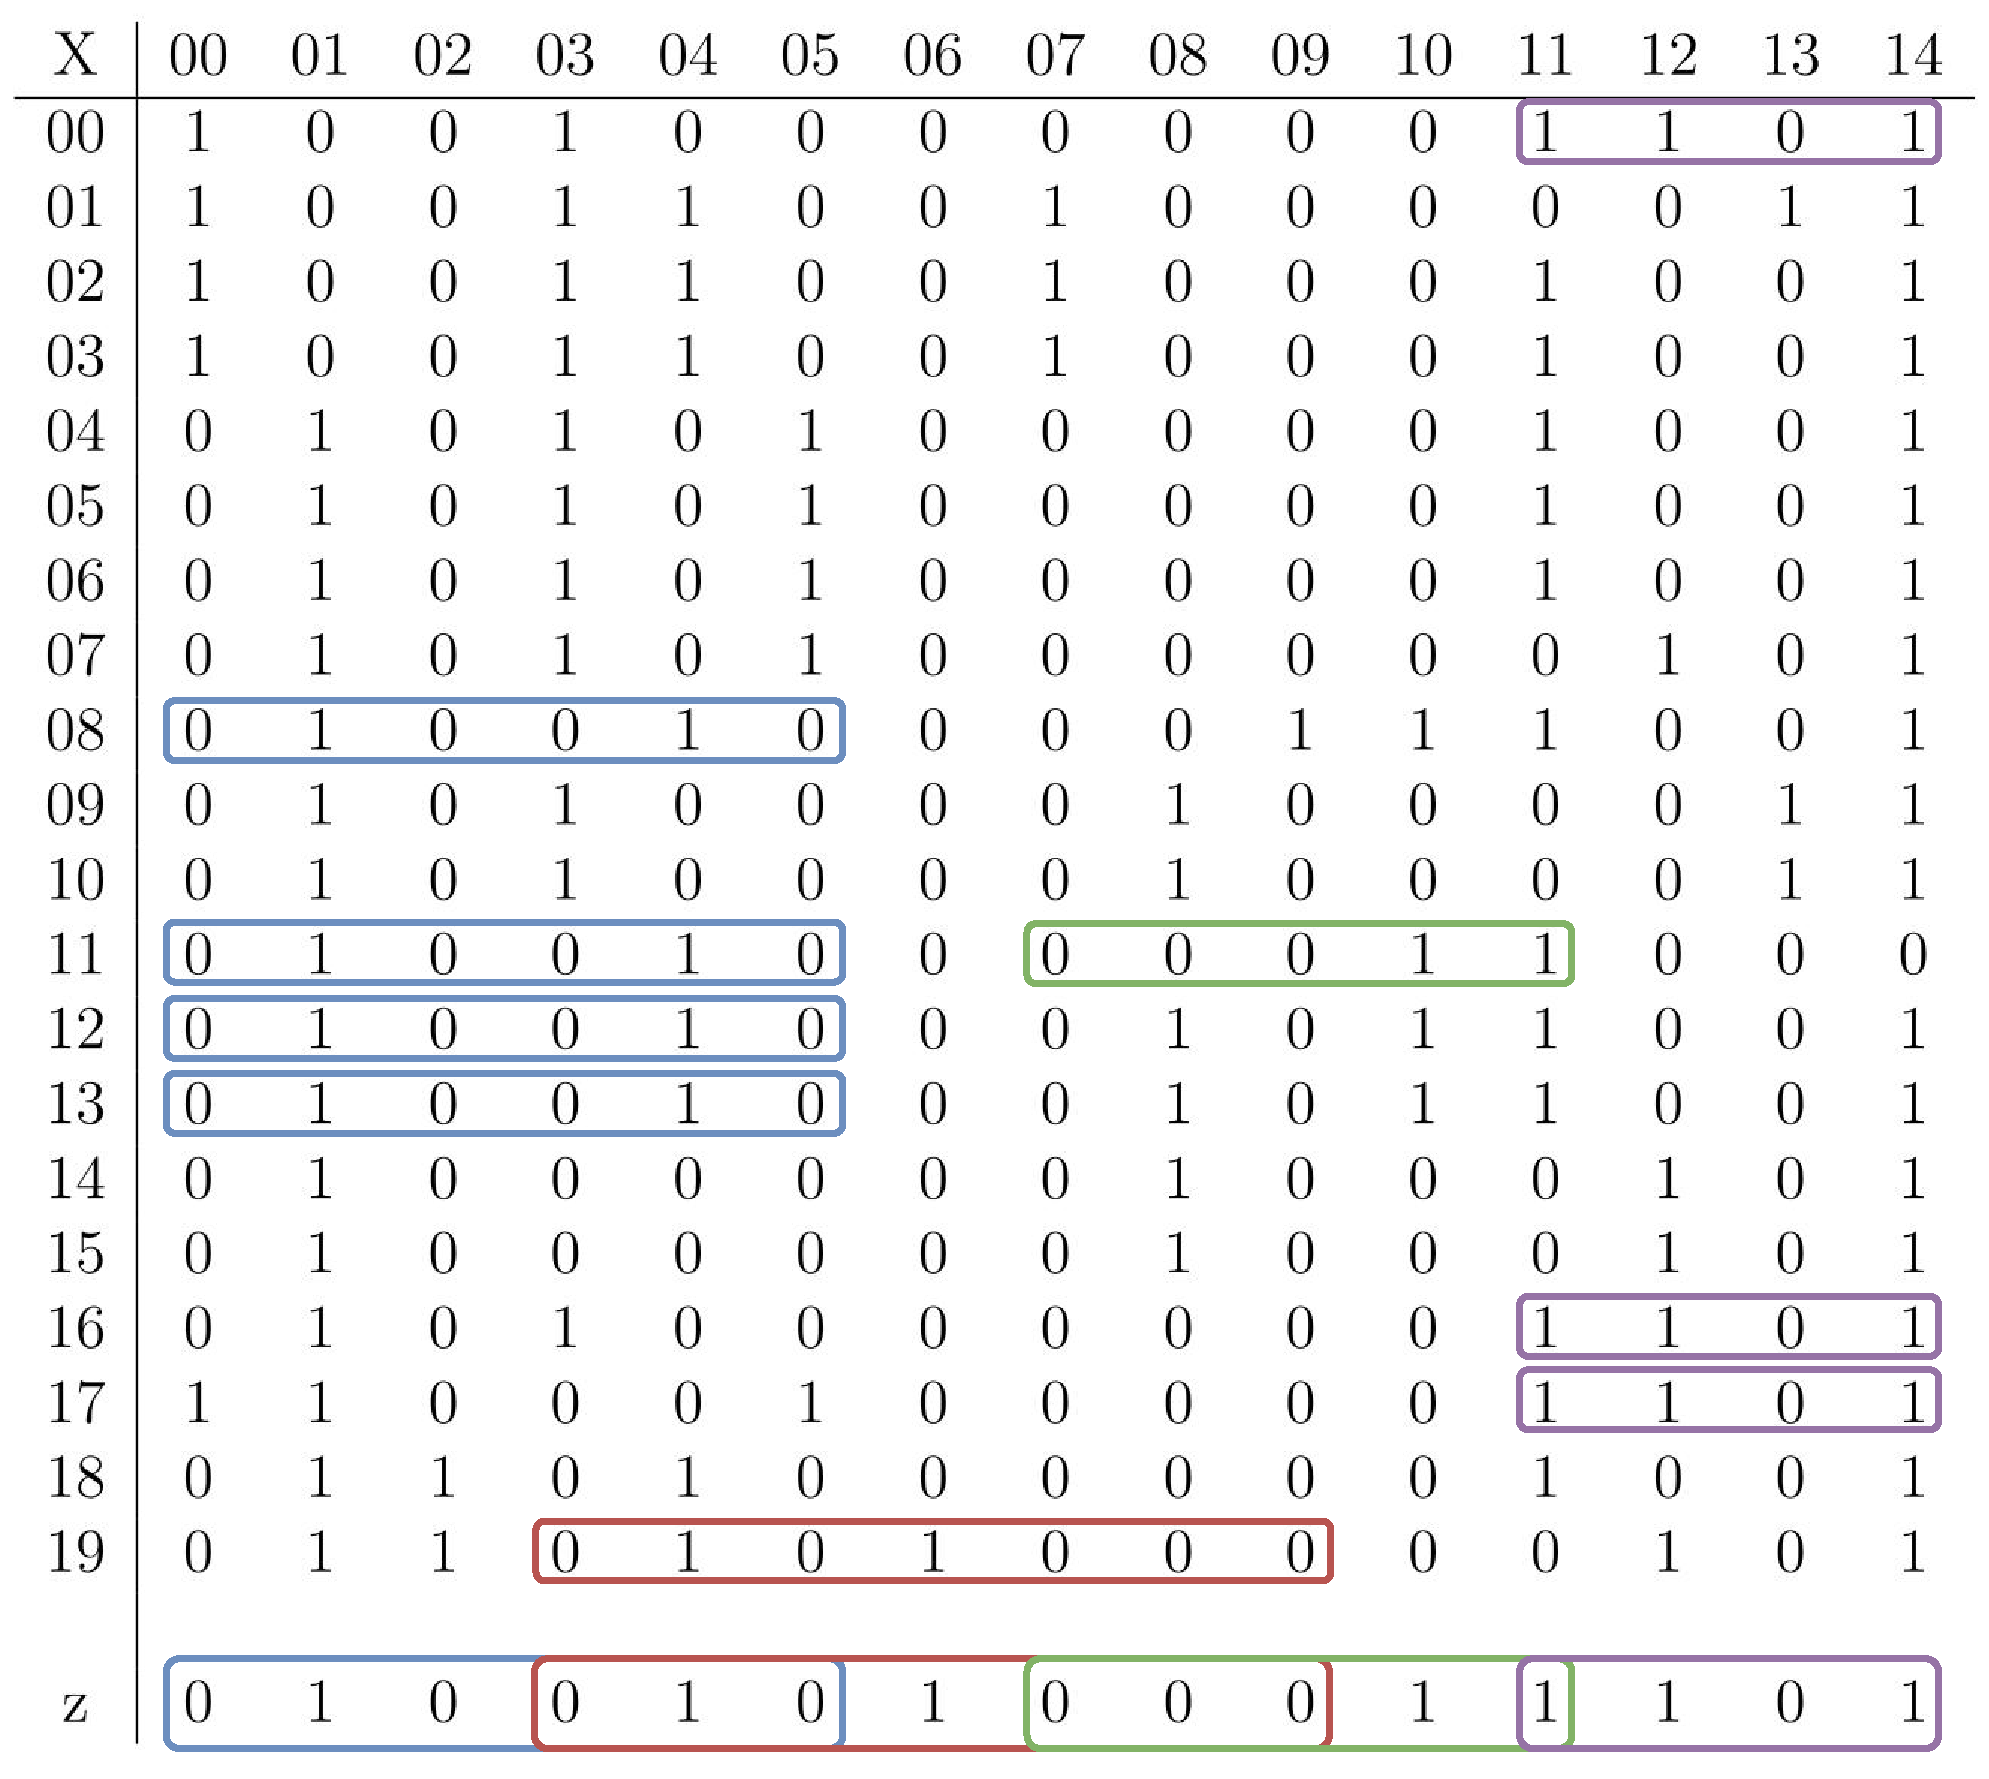
\includegraphics[scale = 0.365]{img/pbwtmatch.pdf}
  \end{figure}
  In tal caso l'array $MS$ sarebbe, avendo scelto come riga iniziale la 19:
  \begin{table}[H]
    \footnotesize{}
    \centering
    \begin{tabular}{c|ccccccccccccccc}
      $k$ & 00 & 01 & 02 & 03 & 04 &  {\color{nordgreen}05} & 06 & 07 & 08
      &  {\color{nordgreen}09} & 10 &  {\color{nordgreen}11} & 12 & 13
      &  {\color{nordgreen}14} \\
      \hline
      \hline
      $z$ & 0 & 1 & 0 & 0 & 1 &  {\color{nordgreen}0} & 1 & 0 & 0
      &  {\color{nordgreen}0} & 1 &  {\color{nordgreen}1} & 1 & 0
      &  {\color{nordgreen}1} \\
      \hline
      $row$ & 19 & 19 & 16 & 15 & 13 &  {\color{nordgreen}13} & 19 & 19 & 19
      &  {\color{nordgreen}19} & 11 &  {\color{nordgreen}11} & 17 & 17
      &  {\color{nordgreen}17} \\
      $len$ & 1 & 2 & 3 & 4 & 5 & {\color{nordgreen}6} & 4 & 5 & 6
      & {\color{nordgreen}7} & 4 & {\color{nordgreen}5} & 2 & 3
      & {\color{nordgreen}4}\\
    \end{tabular}
  \end{table}
  Dove si possono riconoscere i vari \textit{MEM}, la cui colonna di fine è
  segnalata in verde, secondo la definizione data
  sopra (anche in questo caso i dettagli del calcolo
  verranno esplicitati successivamente). 
\end{esempio}
\subsection{Threshold per la RLPBWT}
Come anticipato una prima strategia per la scelta di una nuova riga $j$, qualora
la precedente riga $i$ comporti un mismatch in colonna $k$ con l'aplotipo query,
avendo $x_i[k]\neq z[k]$ è l'utilizzo delle \textbf{threshold}.
\begin{definizione}
  Data la colonna $k$-esima della \textbf{matrice PBWT}, $y^k$, memorizzata
  tramite compressione \textbf{run-length} e data la run $j$-esima, indicizzata
  da $i$ a $i'$, si definisce \textbf{threshold} come l'indice del minimo valore
  \textit{LCP}, che ricordiamo essere calcolato sull'ordinamento inverso,
  compreso negli indici della run, compreso l'eventuale 
  $LCP_k[i'+1]$, qualora $i'\neq M-1$. Si noti che quest'ultimo valore, se
  esistente, deve essere considerato in quanto per il suo calcolo, come
  specificato nei preliminari alla sezione \ref{secpbwt}, si prende in
  considerazione $y^k_{i'}$ e $y^k_{i'+1}$.
\end{definizione}
Con tale informazione, unita ai \textit{prefix array sample}, si può quindi
ottenere un comportamento analogo a quanto si ottiene con l'\textbf{R-index} per
la \textit{RLBWT}.\\
Sia infatti data $t$ la posizione della \textit{threshold} nella run corrente,
in colonna $k$, e
si supponga che tale run, con testa all'indice $h$, non sia associata al simbolo
desiderato, ovvero $z[k]$. Si supponga che, con il mapping, si sia arrivati
all'indice $i$ della colonna $k$. Si supponga inoltre che la run successiva
abbia testa in indice $e$. Si hanno due casi possibili, denotando con
$LCS(x,y)$ il \textit{longest common suffix} tra le stringhe $X$ e $Y$ e con
$a_k$ il \textit{prefix array} in colonna $K$:
\begin{enumerate}
  \item $i<t$ allora, per definizione di \textit{threshold}:
  \[LCS(z[0,k], x_{a_{k}[h-1]}[0,k])\geq LCS(z[0,k], x_{a_{k}[e]}[0,k])\]
  Quindi si ha che $MS[k].row=a_{k}[h-1]$ e il mapping potrà proseguire
  dall'indice $h-1$
  \item  $i\geq t$ allora, per definizione di \textit{threshold}:
  \[LCS(z[0,k], x_{a_{k}[h-1]}[0,k])\leq LCS(z[0,k], x_{a_{k}[e]}[0,k])\]
  Quindi si ha che $MS[k].row=a_{k}[e]$ e il mapping potrà proseguire
  dall'indice $e$
\end{enumerate}
Qualora una colonna presenti solo simboli $\sigma\neq z[k]$, per convenzione, si
imposta che $MS[k].row = M$ e si ricomincia, in colonna $k+1$, dall'ultima
posizione, indicizzata nel pannello originale dal valore finale del
\textit{prefix array sample} dell'ultima run.\\
In termini implementativi anche le posizioni delle \textit{threshold} vengono
memorizzate tramite un \textit{bitvector sparso} per ogni colonna $k$, avendo
che, qualora il minimo \textit{LCP} si ritrovi nell'indice della testa della run
successiva, la posizione della threshold verrà comunque memorizzata all'indice
della coda della run corrente. Purtroppo questa è una situazione di ambiguità,
avendo che, seguendo la definizione sopra, avendo la \textit{threshold} a fine
run, bisognerebbe scegliere la testa della run successiva, qualora l'indice $i$
si trovi esattamente a fine run. Invece, qualora la
\textit{threshold} sia a fine run a causa del fatto che il minimo \textit{LCP}
si trovi nella testa della run successiva, bisogna scegliere la coda della run
precedente. L'unico modo per disambiguare è quindi effettuare \textit{random
  access} al pannello per vedere quale sia la
soluzione migliore, ovvero quale tra la coda della run precedente e la testa
della run successiva siano relative alla riga del pannello originale con un
suffisso comune alla query più lungo.\\
Purtroppo non è possibile salvare la threshold direttamente nella testa della
run successiva in quanto questa potrebbe essere anche la posizione della
threshold della run successiva e avere due threshold sovrapposte impedirebbe di
capire a quale run appartiene una certa threshold, tramite la funzione
\textit{rank}. \\
Tale bitvector deve essere quindi aggiunto alle informazioni memorizzate per
ogni singola colonna. Lo pseudocodice per la costruzione di una colonna con
anche il bitvector per le \textit{threshold} è consultabile all'algoritmo
\ref{algo:cosbv}. 
\begin{esempio}
  \label{es:thr}
  Si vede quindi un esempio di funzionamento delle threshold.\\
  Si prenda pannello visto all'esempio \ref{es:pbwt1} e si effettui la
  permutazione secondo $a_2$:
  \begin{table}[H]
    \centering
    \footnotesize
    \begin{tabular}{c|cc|c|cccccccccccc}
      X & 00 & 01 & 02 & 03 & 04 & 05 & 06 & 07 & 08 & 09 & 10 & 11 & 12 & 13
      & 14 \\
      \hline
      00 & 1 & 0 & 0 & 1 & 0 & 0 & 0 & 0 & 0 & 0 & 0 & 1 & 1 & 0 & 1 \\
      01 & 1 & 0 & 0 & 1 & 1 & 0 & 0 & 1 & 0 & 0 & 0 & 0 & 0 & 1 & 1 \\
      02 & 1 & 0 & 0 & 1 & 1 & 0 & 0 & 1 & 0 & 0 & 0 & 1 & 0 & 0 & 1 \\
      03 & 1 & 0 & 0 & 1 & 1 & 0 & 0 & 1 & 0 & 0 & 0 & 1 & 0 & 0 & 1 \\
      04 & 0 & 1 & 0 & 1 & 0 & 1 & 0 & 0 & 0 & 0 & 0 & 1 & 0 & 0 & 1 \\
      05 & 0 & 1 & 0 & 1 & 0 & 1 & 0 & 0 & 0 & 0 & 0 & 1 & 0 & 0 & 1 \\
      06 & 0 & 1 & 0 & 1 & 0 & 1 & 0 & 0 & 0 & 0 & 0 & 1 & 0 & 0 & 1 \\
      07 & 0 & 1 & 0 & 1 & 0 & 1 & 0 & 0 & 0 & 0 & 0 & 0 & 1 & 0 & 1 \\
      08 & 0 & 1 & 0 & 0 & 1 & 0 & 0 & 0 & 0 & 1 & 1 & 1 & 0 & 0 & 1 \\
      09 & 0 & 1 & 0 & 1 & 0 & 0 & 0 & 0 & 1 & 0 & 0 & 0 & 0 & 1 & 1 \\
      10 & 0 & 1 & 0 & 1 & 0 & 0 & 0 & 0 & 1 & 0 & 0 & 0 & 0 & 1 & 1 \\
      11 & 0 & 1 & 0 & 0 & 1 & 0 & 0 & 0 & 0 & 0 & 1 & 1 & 0 & 0 & 0 \\
      12 & 0 & 1 & 0 & 0 & 1 & 0 & 0 & 0 & 1 & 0 & 1 & 1 & 0 & 0 & 1 \\
      13 & 0 & 1 & 0 & 0 & 1 & 0 & 0 & 0 & 1 & 0 & 1 & 1 & 0 & 0 & 1 \\
      14 & 0 & 1 & 0 & 0 & 0 & 0 & 0 & 0 & 1 & 0 & 0 & 0 & 1 & 0 & 1 \\
      15 & 0 & 1 & 0 & 0 & 0 & 0 & 0 & 0 & 1 & 0 & 0 & 0 & 1 & 0 & 1 \\
      16 & 0 & 1 & 0 & 1 & 0 & 0 & 0 & 0 & 0 & 0 & 0 & 1 & 1 & 0 & 1 \\
      17 & 0 & 1 & 1 & 0 & 1 & 0 & 0 & 0 & 0 & 0 & 0 & 1 & 0 & 0 & 1 \\
      18 & 0 & 1 & 1 & 0 & 1 & 0 & 1 & 0 & 0 & 0 & 0 & 0 & 1 & 0 & 1 \\
      19 & 1 & 1 & 0 & 0 & 0 & 1 & 0 & 0 & 0 & 0 & 0 & 1 & 1 & 0 & 1 \\
    \end{tabular}
  \end{table}
  Si prenda la seconda run, di simboli $\sigma=1$, indicizzata tra 17 e 18. \\
  Si supponga che, tramite il mapping, si sia arrivati alla riga 17 ma che si
  abbia $z[2]=0$. la scelta è quindi tra la coda della run precedente, avendo
  che $a_2[16]=16$ o la testa della run successiva, avendo che $a_2[19]=17$. Si
  può notare come il minimo \textit{LCP} si trovi, per la 
  run, all'indice 18 (a causa del fatto che il minimo \textit{LCP} è all'indice
  19, quello della testa della run successiva). Si può quindi proseguire o con
  la riga. Questo significa che il suffisso comune più lungo con la query si ha
  con la riga 16 del pannello, per definizione di threshold, avendo che questa
  sarà memorizzata nell'array $MS$:
  \[MS[2].row=16\]
  Successivamente, tramite \textit{random access} al testo, confrontando la riga
  $x_{16}$ e la query $z$, fino alla colonna $k=2$, si potrà calcolare che
  $MS[2].len=3$. 
\end{esempio}
\textbf{SISTEMARE ESEMPIO}\\
Una volta computato tutti i valori $MS[i].row$ per calcolare i vari $MS[i].len$
si scorre da sinistra a destra calcolando la lunghezza del match facendo random
access al pannello e confrontando la query $z$ con la riga $MS[i].row$. Si
assuma infatti di aver calcolato $MS[i-1].len$ e di voler calcolare $MS[i].len$.
Si hanno tre casi possibili:
\begin{enumerate}
  \item $MS[i].row=M$ e in tal caso, avendo segnalata l'inesistenza di alcun
  match, si ha che $MS[i].len=0$
  \item $MS[i].row=MS[i-1].row$, avendo $i\neq 0$ e $MS[i-1].len\neq 0$, allora
  si sta seguendo la stessa riga che si seguiva in colonna $i-1$ e quindi,
  banalmente, $MS[i].len=MS[i-1].len+1$
  \item in qualsiasi altro caso bisogna confrontare, a partire dalla colonna
  $i$, la query 
  $z$ con la riga $MS[i].row$ del pannello da destra a sinistra, fino a che non
  si trova un mismatch, calcolando la lunghezza $l$ del suffisso comune tra esse
  e memorizzando tale valore: $MS[i].len=l$
\end{enumerate}
In fase di costruzione delle lunghezze è possibile anche riportare i
\textit{MEM}, terminanti in colonna $i$, qualora:
\begin{itemize}
  \item $MS[i].len\geq MS[i+1].len \land MS[i].len\neq 0$
  \item si è arrivati a fine array, avendo $i=N-1\land MS[i].len\neq 0$
\end{itemize}
Come si può verificare nell'esempio \ref{es:ms}.\\
L'algoritmo per il match tramite \textit{threshold} è visualizzabile
all'algoritmo \ref{algo:matchthr}.
\textbf{CAPIRE SE DESCRIVERE ALGORITMO}
\subsection{LCE query per la RLPBWT}
La memorizzazione di un \textit{bitvector sparso} atto a rappresentare le
posizioni delle threshold ha però un costo in memoria. Inoltre, per ora, si è
parlato di tenere in memoria il pannello sotto forma di vettore di
\textit{bitvector} e anche questo ha un costo non indifferente in termini di
spazio necessario.\\
Per arrivare all'implementazione conclusiva della \textit{RLPBWT} si è quindi
optato per la memorizzazione del pannello sotto forma di \textit{SLP}, struttura
che, come anticipato, permette anche di eseguire efficientemente le \textit{LCE
  query}.
\begin{definizione}
  Dato un pannello $X$, $M\times N$, e due righe $x_i$ e $x_j$ tali che $0\leq
  i <m$ e $0\leq j <M$, con $i\neq j$, si definisce \textbf{LCE query} il
  suffisso comune più lungo tra le due stringhe. Per comodità nella sezione si
  definisce la funzione: 
  \[LCE_k(x_i,x_j)=l\]
  dove $l$ è la lunghezza del suffisso comune più lungo tra le due stringhe
  terminante in colonna $k-1$.
\end{definizione}
\subsubsection{Compressione del panel}
Bisogna quindi capire in primis come costruire l'\textit{SLP}. In primis, le
librerie per la costruzione di tale struttura assumono un input
``monodimensionale'', ovvero una singola sequenze lineare. Inoltre, anche per
permettere la costruzione efficiente della \textit{PBWT}, e conseguentemente
della \textit{RLPBWT}, il pannello in input risulta essere trasposto, avendo che
le righe nel file in input rappresentano i siti e non gli individui. Bisogna
quindi in primis trasporre tale pannello. Per procedere ulteriormente bisogna
però ricordare che sull'\textit{SLP} si avrà 
necessità di effettuare \textit{LCE query} che però, si anticipa, nel nostro
pannello, devono essere fatte tra due righe da destra a sinistra (a differenza
di quanto visto nel caso standard dove si confrontavano prefissi comuni). Per
rendere possibile questa operazione quindi il pannello deve essere sia 
salvato come un'unica riga, per ottenerne l'\textit{SLP}, che ``da destra a
sinistra'', per permettere le \textit{LCE query}. Si procede quindi concatenando
ogni riga, selezionandole consecutivamente e leggendone i singoli elementi da
destra a sinistra.
\begin{esempio}
  Si vede quindi un breve esempio.\\
  Si assuma di avere il seguente pannello nel file in input.
  \[
    X=\left[
      \begin{matrix}
        0 & 0 & 1 & 0 & 0\\
        1 & 1 & 1 & 0 & 1\\
        0 & 1 & 1 & 1 & 1\\
        0 & 0 & 0 & 1 & 0
      \end{matrix}
    \right]
  \]
  Dove però come detto le righe sono i siti e le colonne i sample. Per ottenere
  l'\textit{SLP} biosgna quindi, in primis, trasporre la matrice:
  \[
    X^T=\left[
      \begin{matrix}
        0 & 1 & 0 & 0\\
        0 & 1 & 1 & 0\\
        1 & 1 & 1 & 0\\
        0 & 0 & 1 & 1\\
        0 & 1 & 1 & 0
      \end{matrix}
    \right]
  \]
  A questo punto bisogna considerare l'ordine in cui si vorranno effettuare le
  \textit{LCE query}.
  Ad esempio, prendendo la seconda e la terza riga, facendo partire il confronto
  dall'ultima colonna, avremmo una \textit{LCE
    query} lunga 3, terminante nella prima colonna esclusa:
  \begin{figure}[H]
    \centering
    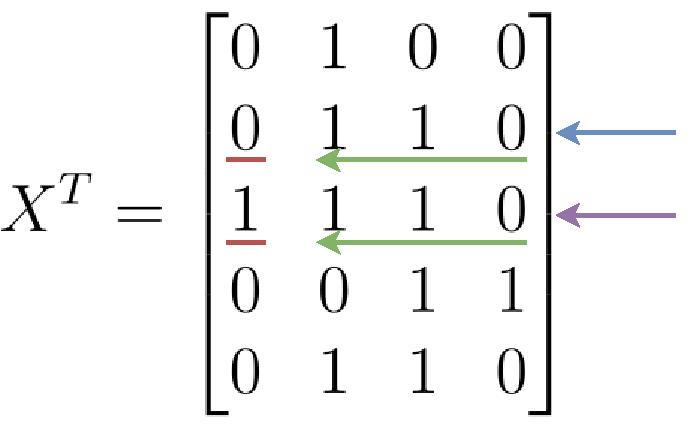
\includegraphics[scale = 0.38]{img/slppanel.pdf}
  \end{figure}
  Si procede quindi salvano la sequenza lineare relativa al pannelli come
  descritto sopra,
  ottenendo, con colorate gli stessi risultati della query fatta
  sopra:
  \[0010\,\,{\color{nordgreen}011}{\color{nordred}0}\,\,
    {\color{nordgreen}011}{\color{nordred}1} \,\,1100\,\,0110\]
  \textit{Si noti che qui si sono segnalate le varie righe con uno spazio ma
    solo per praticità ``visiva''.}
\end{esempio}
\textbf{ESEMPIO MAGARI DA SCRIVERE MEGLIO}
\subsubsection{LCE query}
Grazie all'uso delle \textit{LCE query} è quindi possibile calcolare l'array
delle \textit{matching statistics} in un solo scorrimento da sinistra a
destra. Infatti è possibile usare tali query per calcolare non solo quale nuova
sequenza scegliere in caso di mismatch con l'aplotipo query in colonna $i$, come
si faceva con l'uso delle \textit{threshold}, ma anche di computare la lunghezza
del suffisso comune tra essa e l'aplotipo query, calcolando nello stesso momento
sia $MS[i].row$ che $MS[i].len$.\\
Anche in questo caso, per convenzione, si inizia la computazione dell'ultima
riga della prima colonna.\\
Si illustra ora come computare l'array delle \textit{matching statistics}.
Si assuma di avere calcolato l'array $MS$ di una query $z$ rispetto al pannello
$X$. le cui righe si identificano tramite $x_i, \forall i\in\{0,M\}$, fino alla
colonna $k-1$. Sia $i$ 
l'indice di riga sulla \textit{matrice PBWT} al quale si è arrivati mediante il
mapping, avendo che tale riga è quella che ha il più lungo suffisso comune con
$z[1,k-1]$. Si assuma che l'indice $i$ appartenga alla run $r$, di simboli
$\sigma$, testa di indice $h$ e coda di indice $e-1$. Si hanno diversi casi:
\begin{enumerate}
  \item $z[k]=\sigma$, quindi la riga $i$ può essere usata per estendere il
  match, avendo che $MS[k].row=MS[k-1].row$ e $MS[k].len=MS[k-1].len+1$, e per
  proseguire col mapping in colonna $k+1$
  \item $z[k]\neq\sigma$ e si una sola run in colonna $k$, avendo quindi che non
  si possono avere match. Per convenzione, si
  imposta che $MS[k].row = M$ e $MS[k].len=0$. Infine si ricomincia, in colonna
  $k+1$, dall'ultima posizione, indicizzata nel pannello originale dal valore
  finale del \textit{prefix array sample} dell'ultima run
  \item $z[k]\neq\sigma$ ma si hanno anche altre run, dovendo quindi scegliere
  la nuova riga da seguire. Si ha che il più lungo suffisso di $z[1,k]$ che è
  anche suffisso di $x_1[1,k],\ldots, x_m[1,k]$ è uno tra:
  \begin{itemize}
    \item $x_{a_k[h-1]}$, se $h\neq 0$, ovvero la riga del pannello
    corrispondente alla fine della run precedente a $r$ nella \textit{matrice
      PBWT}, se esistente
    \item $x_{a_k[e+1]}$, se $e\neq M-1$, ovvero la riga del pannello
    corrispondente all'inizio della run successiva a $r$ nella \textit{matrice
      PBWT}, se esistente
  \end{itemize}
  Avendo quindi i \textit{prefix array sample} che ci dicono a quale riga nel
  pannello corrispondano tali valori e conoscendo $MS[k-1].row$ è possibile
  calcolare $LCE(MS[k-1].row, a_k[h-1])$ e $LCE(MS[k-1].row, a_k[e+1])$. A
  questo punto si sceglie il suffisso comune più lungo tra le due, ovvero il
  maggiore tra i valori ritornati dalla \textit{LCE query} e si sceglie la riga
  corrispondente per proseguire. Si ha quindi o $MS[k].row=a_k[h-1]$ o
  $MS[k].row=a_k[e+1]$. In merito alla lunghezza, assumendo che il miglior
  valore ritornato dalle due \textit{LCE query} sia $l$, si ha che:
  \[MS[k].len=\min(MS[k-1].len, l)+1\]
  In quanto la LCE query potrebbe restituire un valore più lungo dell'effettivo
  match con al query $z$ quindi si sceglie il minimo tra le due lunghezze,
  ottenendo l'effettiva lunghezza del suffisso comune tra $z$ e la nuova riga
  scelta fino a $k-1$, e lo si 
  incrementa di uno, contando il match ottenuto in colonna $k$
\end{enumerate}
\textbf{SISTEMARE}
\begin{esempio}
  Riprendiamo l'esempio \ref{es:thr}, visto per il calcolo
  tramite \textit{threshold}. \\
  Senza usare le \textit{threshold}, nella medesima situazione si dovrebbe
  calcolare, avendo che $MS[1].row=19$ e $MS[1].len =2$:
  \[LCE_1(x_{19}, x_{16})=2\]
  \[LCE_1(x_{19}, x_{17})=1\]
  Come verificabile dal pannello presente all'esempio \ref{es:pbwt1}.\\
  Si ha quindi che $MS[2].row=16$. Inoltre, sempre per quanto detto sopra:
  \[MS[2].len=\min(MS[1].len, 2)+1=2+1=3\]
\end{esempio}
Con questa variante quindi:
\begin{itemize}
  \item non si necessita di tenere in memoria le informazioni per le
  \textit{threshold}
  \item si tiene in memoria il pannello sotto forma di \textit{SLP}, soluzione
  vantaggiosa dal punto di vista della memoria anche se svantaggiosa da quello
  temporale (come descritto nella sezione \ref{secslp})
  \item si permette il calcolo dell'array $MS$ in una singola scansione del
  pattern 
\end{itemize}
\textbf{Essendo lo scopo principale della tesi la riduzione dello spazio
  occupato dalla struttura dati questa è la soluzione migliore, avendo in
  memoria una struttura run-length encoded per la PBWT in grado di permettere
  pattern matching con un aplotipo esterno}.


% sezione per struttura phi
\section{Funzione Phi}
\label{secphi}
\subsection{Costruzione della struttura di supporto}
\subsection{Estensione dei match}


\chapter{Risultati}
\label{reschap}
Verranno ora riportati alcuni risultati sperimentali, ottenuti su pannelli
simulati, relativi all'implementazione, in \Cplusplus 11, della \textbf{RLPBWT}.
% sezione strumenti
\paragraph{RLPBWT.}
In merito alle varianti della $\RLPBWT$, sono state testate le otto
strutture dati composte discusse nel capitolo \ref{metchap}:
\begin{enumerate}
  \item la struttura dati composta \texttt{MAP-INT + RLCP} e la struttura dati
  composta \texttt{MAP-BV + RLCP}. Si ricorda che tali soluzioni non supportano
  il riconoscimento delle righe del pannello, per cui si ha uno $\SMEM$, ma
  solo la cardinalità dell'insieme delle stesse
  \item le strutture dati composte basate sull'uso delle threshold per
  il calcolo dell'array delle matching statistics, 
  ovvero: \texttt{MAP-INT + THR-INT + RA-BV + PERM + PHI},  \texttt{MAP-INT +
    THR-INT + RA-SLP + PERM + PHI}, \texttt{MAP-BV + THR-BV + RA-BV + PERM +
    PHI} e \texttt{MAP-BV + THR-BV + RA-SLP + PERM + PHI} 
  \item le strutture dati composte basate sull'uso delle $\LCE$ query
  per
  il calcolo dell'array delle matching statistics,
  ovvero: \texttt{MAP-INT + LCE + PERM + PHI} e \texttt{MAP-BV + LCE + PERM +
    PHI}  
\end{enumerate}
L'implementazione è stata fatta in linguaggio \Cplusplus, usando
librerie esterne:
\begin{itemize}
  \item SDSL per intvector compressi,
  bitvector, bitvector sparsi, serializzazione e varie utility
  per il calcolo della memoria delle strutture dati
  \item BigRePair e ShapedSlp per la costruzione e l'uso degli $\SLP$ 
\end{itemize}
L'implementazione delle strutture composte per la
$\RLPBWT$ supporta lo studio parallelo di più query tramite
openMP \cite{openmp}. Al fine di un più 
corretto confronto con l'implementazione della $\PBWT$,
l'intera sperimentazione è stata
svolta sfruttando un solo thread per volta, tramite la variabile
d'ambiente \texttt{OMP\_NUM\_THREADS=1}.
\paragraph{PBWT.}
Per validare più correttamente i confronti tra le varie strutture dati
per la $\RLPBWT$ e la $\PBWT$ di Durbin, si è scelto di utilizzare
l'implementazione originale di
quest'ultima\footnote{\url{https://github.com/richarddurbin/pbwt}}. Tale
implementazione è scritta in 
linguaggio C e
fornisce tre algoritmi per il calcolo degli $\SMEM$, avendo $N$ siti, $M$ sample
e $Q$ query, per i quali l'autore ha riportato le complessità asintotiche 
nei commenti del codice: 
\begin{enumerate}
  \item \texttt{matchNaive}, ovvero un'implementazione na\"{i}ve del calcolo
  degli $\SMEM$ che non sfrutta la $\PBWT$. Questo algoritmo non è
  utilizzabile in casi reali. La complessità in tempo di tale 
  soluzione è stimata essere $\mathcal{O}(\mathit{NMQ})$ mentre quella in spazio
  è 
  $\mathcal{O}(\mathit{NM})$
  \item \texttt{matchIndexed}, ovvero l'algoritmo 5 del paper originale
  \cite{pbwt}. La complessità in tempo di tale 
  soluzione è stimata essere $\mathcal{O}(\mathit{NQ})$, dopo una fase di
  preprocessing 
  con complessità $\mathcal{O}(\mathit{NM})$. La complessità in spazio è stimata
  essere 
  $\mathcal{O}(\mathit{NM})$, ricordando che essa corrisponde a $13\mathit{NM}$
  byte in memoria
  \item \texttt{matchDynamic}, ovvero un algoritmo non approfondito nel paper,
  ma
  solo citato nei risultati sotto il nome di ``batch''.
  Si è dedotto che il suo funzionamento
  si basa sulla creazione della $\PBWT$ anche delle query, viste 
  sotto forma di pannello, e sull'applicazione dell'algoritmo per il calcolo
  degli $\SMEM$  
  interni alla sua ``fusione virtuale'' con la $\PBWT$ del pannello di aplotipi.
  Inoltre, il calcolo dei vari indici viene
  fatto di colonna in colonna, avendo una sola scansione
  della struttura dati per tutte le query, a differenza dell'algoritmo
  \texttt{matchIndexed} e degli algoritmi per la $\RLPBWT$.
  La complessità in tempo di tale 
  soluzione è stimata essere $\mathcal{O}(N(M+Q))$, mentre quella in spazio è
  $\mathcal{O}(N+M)$. 
\end{enumerate}
Si intuisce fin da subito come l'ultima soluzione, della quale si è avuta
conoscenza solo in fase di
sperimentazione, risulti essere la migliore a disposizione, sia in spazio che
in tempo. Si hanno solo due
limitazioni. La prima è dovuta al fatto che, dovendo computare
la trasformata anche per il pannello di query ed essendo l'algoritmo studiato
per lavorare sulla trasformata stessa, i tempi di calcolo per poche query sono
alti rispetto all'algoritmo \texttt{matchIndexed} e rispetto alle varie
soluzioni per la $\RLPBWT$. Il secondo limite è che i risultati non sono
ordinati, infatti l'algoritmo \texttt{matchDynamic}, studiando la trasformata
anche delle query,
presenta tutti i risultati permutati secondo la stessa, mentre tutti gli altri
algoritmi presentano i risultati query per query. Si rileva
come tali limiti possano essere per lo più trascurabili, nonostante il problema
su
cui si concentrano gli studi di questa tesi sia la ricerca degli $\SMEM$ tra
una 
singola query e un pannello di aplotipi.
\section{Pannelli del 1000 Genome Project}
Come anticipato, al fine di valorizzare i risultati teorici ottenuti in
questo progetto, si 
è deciso di procedere con lo studio di dati reali, relativi alla phase
  3 del 1KGP
\footnote{\url{https://ftp.1000genomes.ebi.ac.uk/vol1/ftp/release/20130502/}}
\cite{1kgp}.\\ 
Tali pannelli, disponibili in formato VCF (Variant Call Format) \cite{vcf},
presentano un numero 
costante di sample, ovvero 5.008, mentre varia il numero di siti. Essendo
dati reali, si ha anche la presenza di siti multiallelici. Si è quindi proceduto
alla selezione dei soli siti biallelici, ottenendo pannelli costruiti su
un alfabeto binario $\Sigma=\{0,1\}$, tramite l'uso di bcftools
\cite{bcftools}, con il comando \texttt{bcftools view -m2 -M2
  -v snps}.\\
Si sono scelti i pannelli relativi ai cromosomi 22 (\texttt{chr22}), 20
(\texttt{chr20}), 18 (\texttt{chr18}), 16 (\texttt{chr16}) e 1 (\texttt{chr1}).
Si noti che  
l'ordine è dato dal numero crescente di siti e che la scelta di includere il
cromosoma 1 è dettata dal fatto che è il più grande cromosoma
umano, quindi  anche il relativo pannello delle varianti geniche
è tra quelli col maggior numero di siti, mentre gli altri sono stati scelti
per praticità, in quanto pannelli non troppo estesi.\\
Trattandosi di pannelli reali, è risultata interessante una preliminare
indagine esplorativa sulla natura di tali pannelli in termini di
sparsità degli alleli e di conseguente numerosità attesa delle run. Si è
quindi calcolato, per i cinque pannelli, il numero di simboli $\sigma=0$ e
$\sigma=1$, notando come il numero di simboli $\sigma=1$ fosse molto ridotto
rispetto al totale ($\sim 0.03\%$ del totale in tutti e
cinque i casi). Una tale
sparsità del dato ha diretta conseguenza sul numero di run di ogni
colonna. Infatti, avendo 
pochi simboli $\sigma=1$ in ogni colonna, che possono anche
essere nella medesima run dopo la permutazione data dalla
$\PBWT$, si producono, nel complesso, poche run. Si ricordi, inoltre, che tale
permutazione, come la 
$\BWT$, è studiata per essere 
maggiormente efficiente nel caso del dato biologico, comportando un'alta
probabilità di produrre run del medesimo carattere. In tabella \ref{tab:panel}
si riportano il numero di siti di ogni cromosoma, il 
numero medio di run per colonna, il numero 
massimo di run in una colonna e il totale delle run. Si segnala, inoltre,
come la
mediana del numero di run per colonna abbia valore 3 per tutti e tre i pannelli.
I valori quantitativi sono 
stati calcolati a partire dai pannelli con un numero di sample pari a 4.908,
poiché 100 sample/righe sono state utilizzate come query nelle successive
fasi della sperimentazione.
\begin{table}
  \centering
  \caption{Informazioni quantitative relative ai cinque pannelli in analisi.}
  \label{tab:panel}
  \vspace{-2mm}
  \begin{tabular}{c||c|c|c|c}
    \textbf{Chr} & \textbf{\#Siti} & \textbf{\#Run totale}
    & \textbf{Max run} & \textbf{Media run} \\ 
    \hline
    \texttt{chr22} & 1.055.454 & 14.772.105 & 2.450 & 14\\
    \texttt{chr20} & 1.739.315 & 19.966.504 & 2.176 & 11\\
    \texttt{chr18} & 2.171.378 & 24.288.263 & 2.365 & 11\\
    \texttt{chr16} & 2.596.072 & 31.187.856 & 2.330 & 12\\
    \texttt{chr1} & 6.196.151 & 69.671.952 & 2.721 & 11\\
  \end{tabular}
\end{table}
In merito alla sparsità del dato e al
conseguente basso numero medio di run per colonna, si conferma il risultato
atteso che è a favore, in termini di 
complessità in spazio/tempo, della $\RLPBWT$, in quanto tutte le componenti sono
proporzionali, al numero di run (a eccezione della componente \texttt{RLCP}). In
figura 
\ref{fig:boxplot} si riportano i risultati statistici, sotto forma di
boxplot, relativi alla distribuzione delle run nei cinque pannelli
studiati. Il forte numero di outlier si ha poiché media e 
mediana del numero di run per colonna risultano essere molto piccole rispetto al
numero massimo di run riscontrabili in una colonna.
\begin{figure}
  \centering
  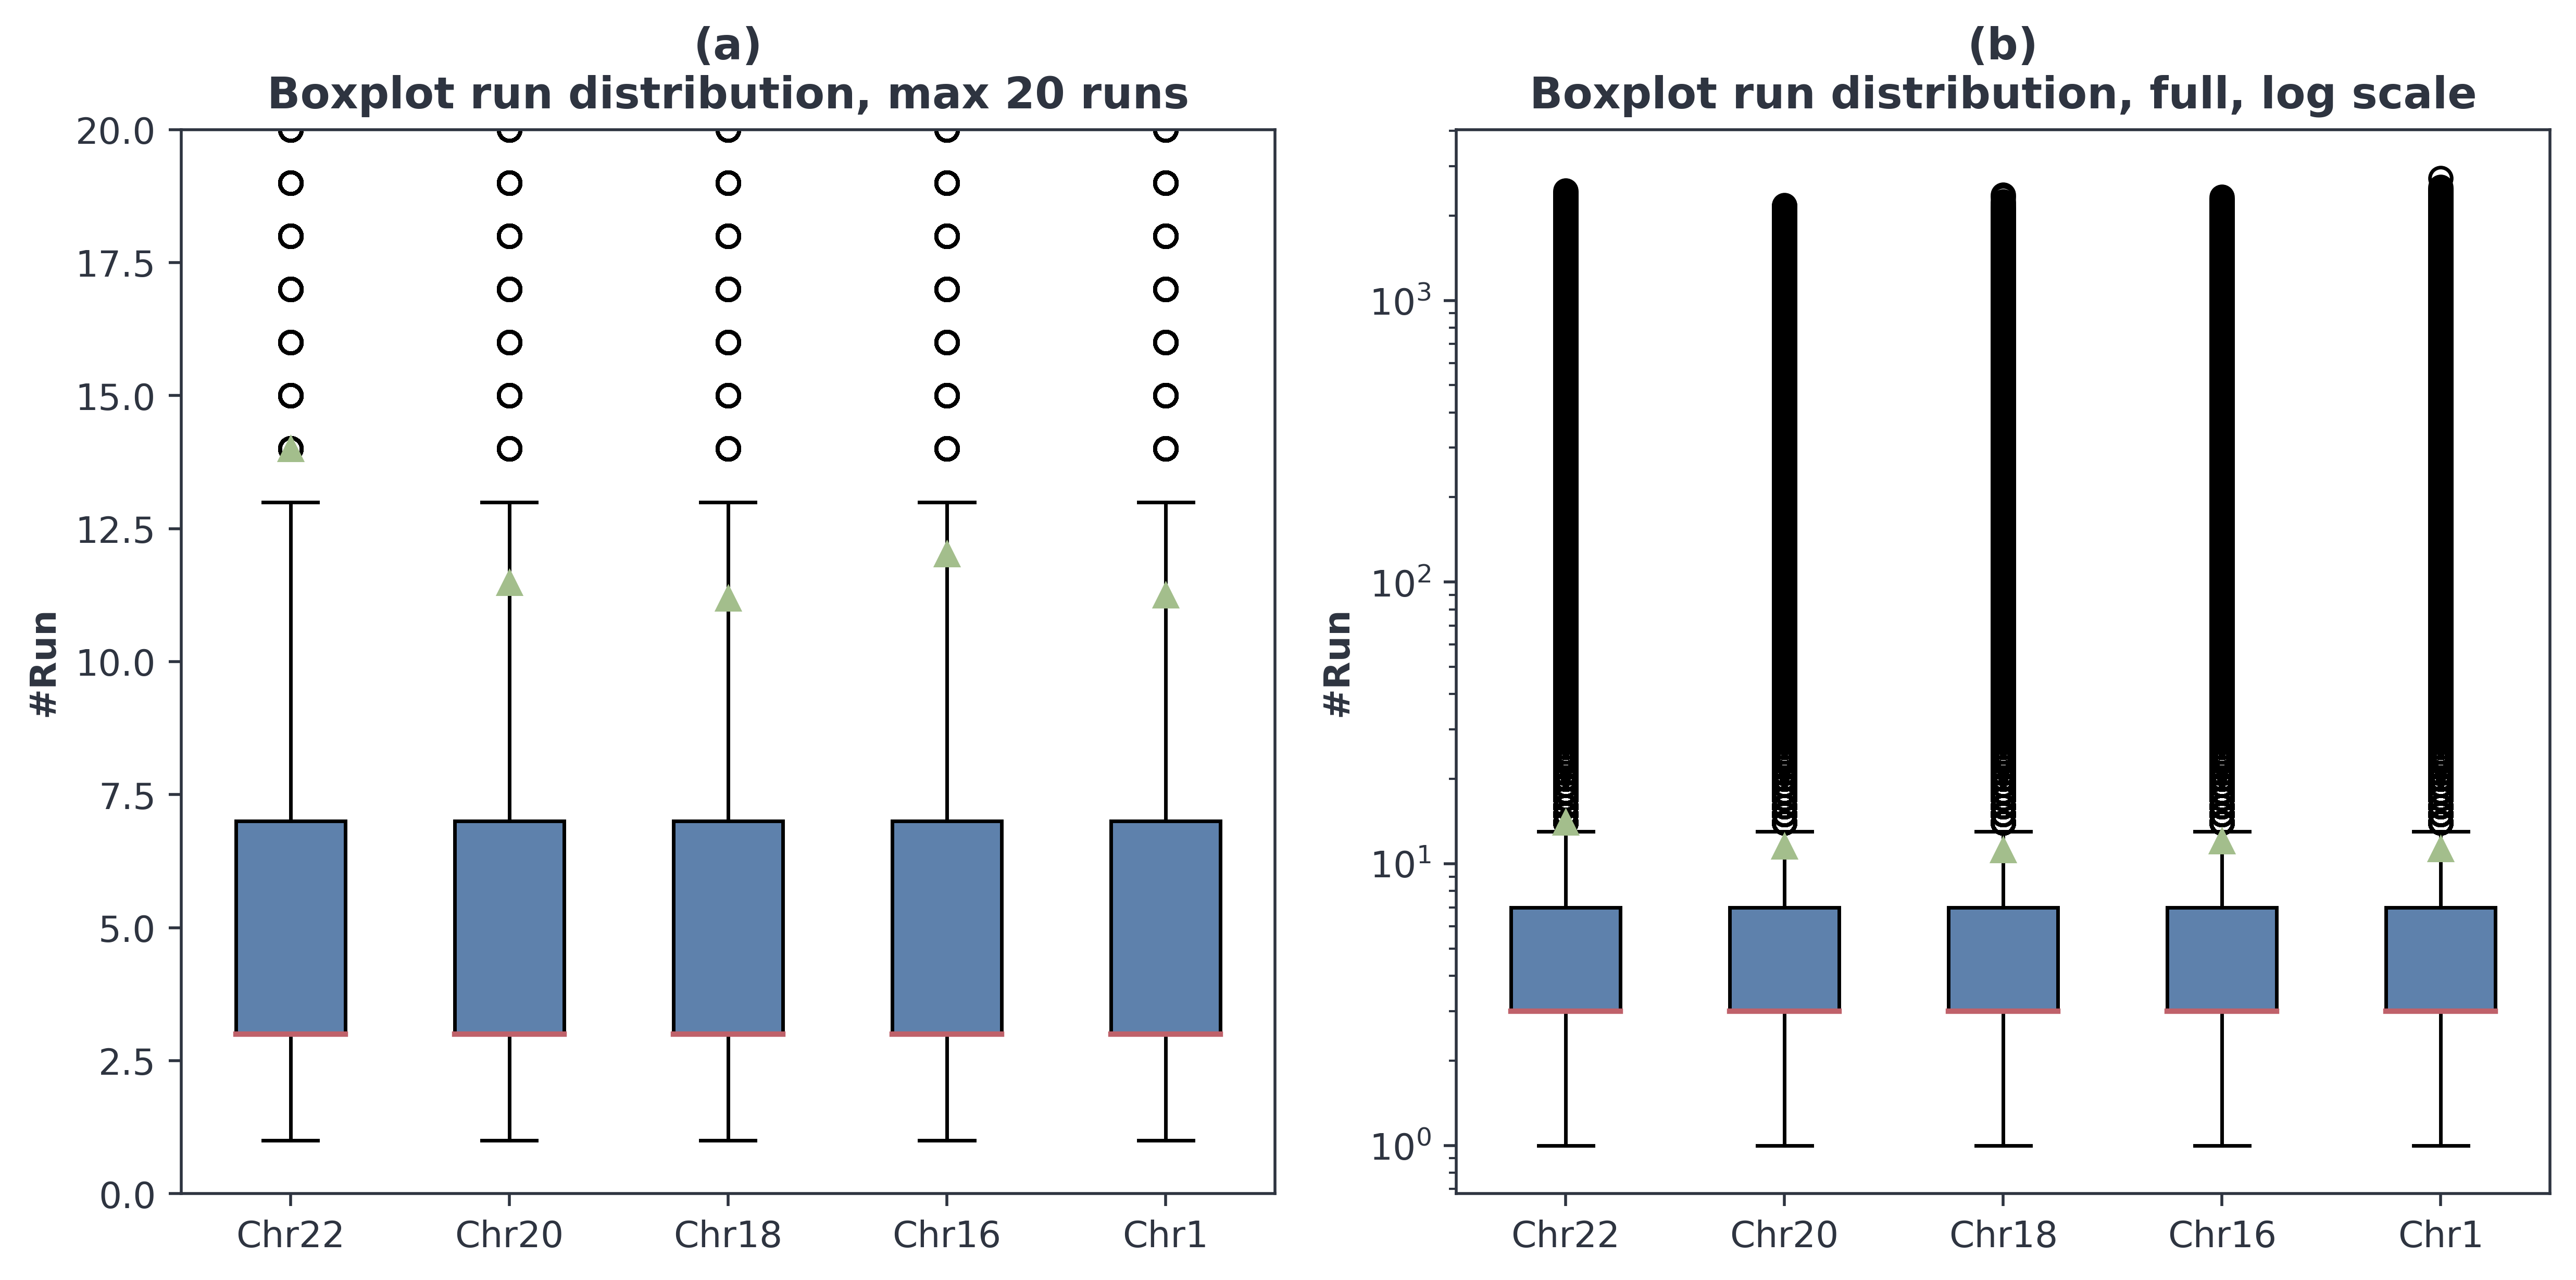
\includegraphics[width = \linewidth]{img/boxplotbi.png}
  \vspace{-5mm}
  \caption{Boxplot della distribuzione delle run per i pannelli dei cinque
    cromosomo studiati. Il grafico (a) presenta uno zoom che esclude la maggior
    parte degli outlier mentre il grafico (b) presenta, in scala logaritmica, il
    boxplot completo con tutti gli outlier.}
  \label{fig:boxplot}
\end{figure}
\subsection{Riproducibilità degli esperimenti}
Al fine di rendere riproducibili gli esperimenti, si è costruita una pipeline
per l'esecuzione dei vari algoritmi e l'estrazione dei dati quantitativi
relativi alle
performance\footnote{\url{https://github.com/dlcgold/rlpbwt-test}}.\\
L'intera pipeline è stata gestita tramite Snakemake \cite{snakemake}
(un workflow management system), uno strumento molto usato in
bioinformatica per creare analisi dati scalabili e riproducibili. Nel
dettaglio la pipeline comprende, come visualizzabile in figura \ref{fig:snake},
avendo in input una lista di pannelli con associato il numero di query:
\begin{itemize}
  \item lo scaricamento dei tool e delle dipendenze per la $\PBWT$ di
  Durbin e la $\RLPBWT$ proposta in questa tesi
  \item la produzione dell'input per la $\PBWT$ e per le varianti della
  $\RLPBWT$, in base alla quantità di query richiesta
  \item la produzione delle strutture dati
  \item l'esecuzione degli algoritmi per il calcolo degli $\SMEM$
  % \item produzione di vari grafici relativi sia ai tempi di esecuzione che alla
  % memoria richiesta
\end{itemize}
Si è deciso di estrarre dai pannelli un numero di righe pari al numero di 
query richieste, che, a loro volta, andranno a formare il pannello di
query, in modo che il calcolo non sia banale.\\
\begin{figure}
  \centering
  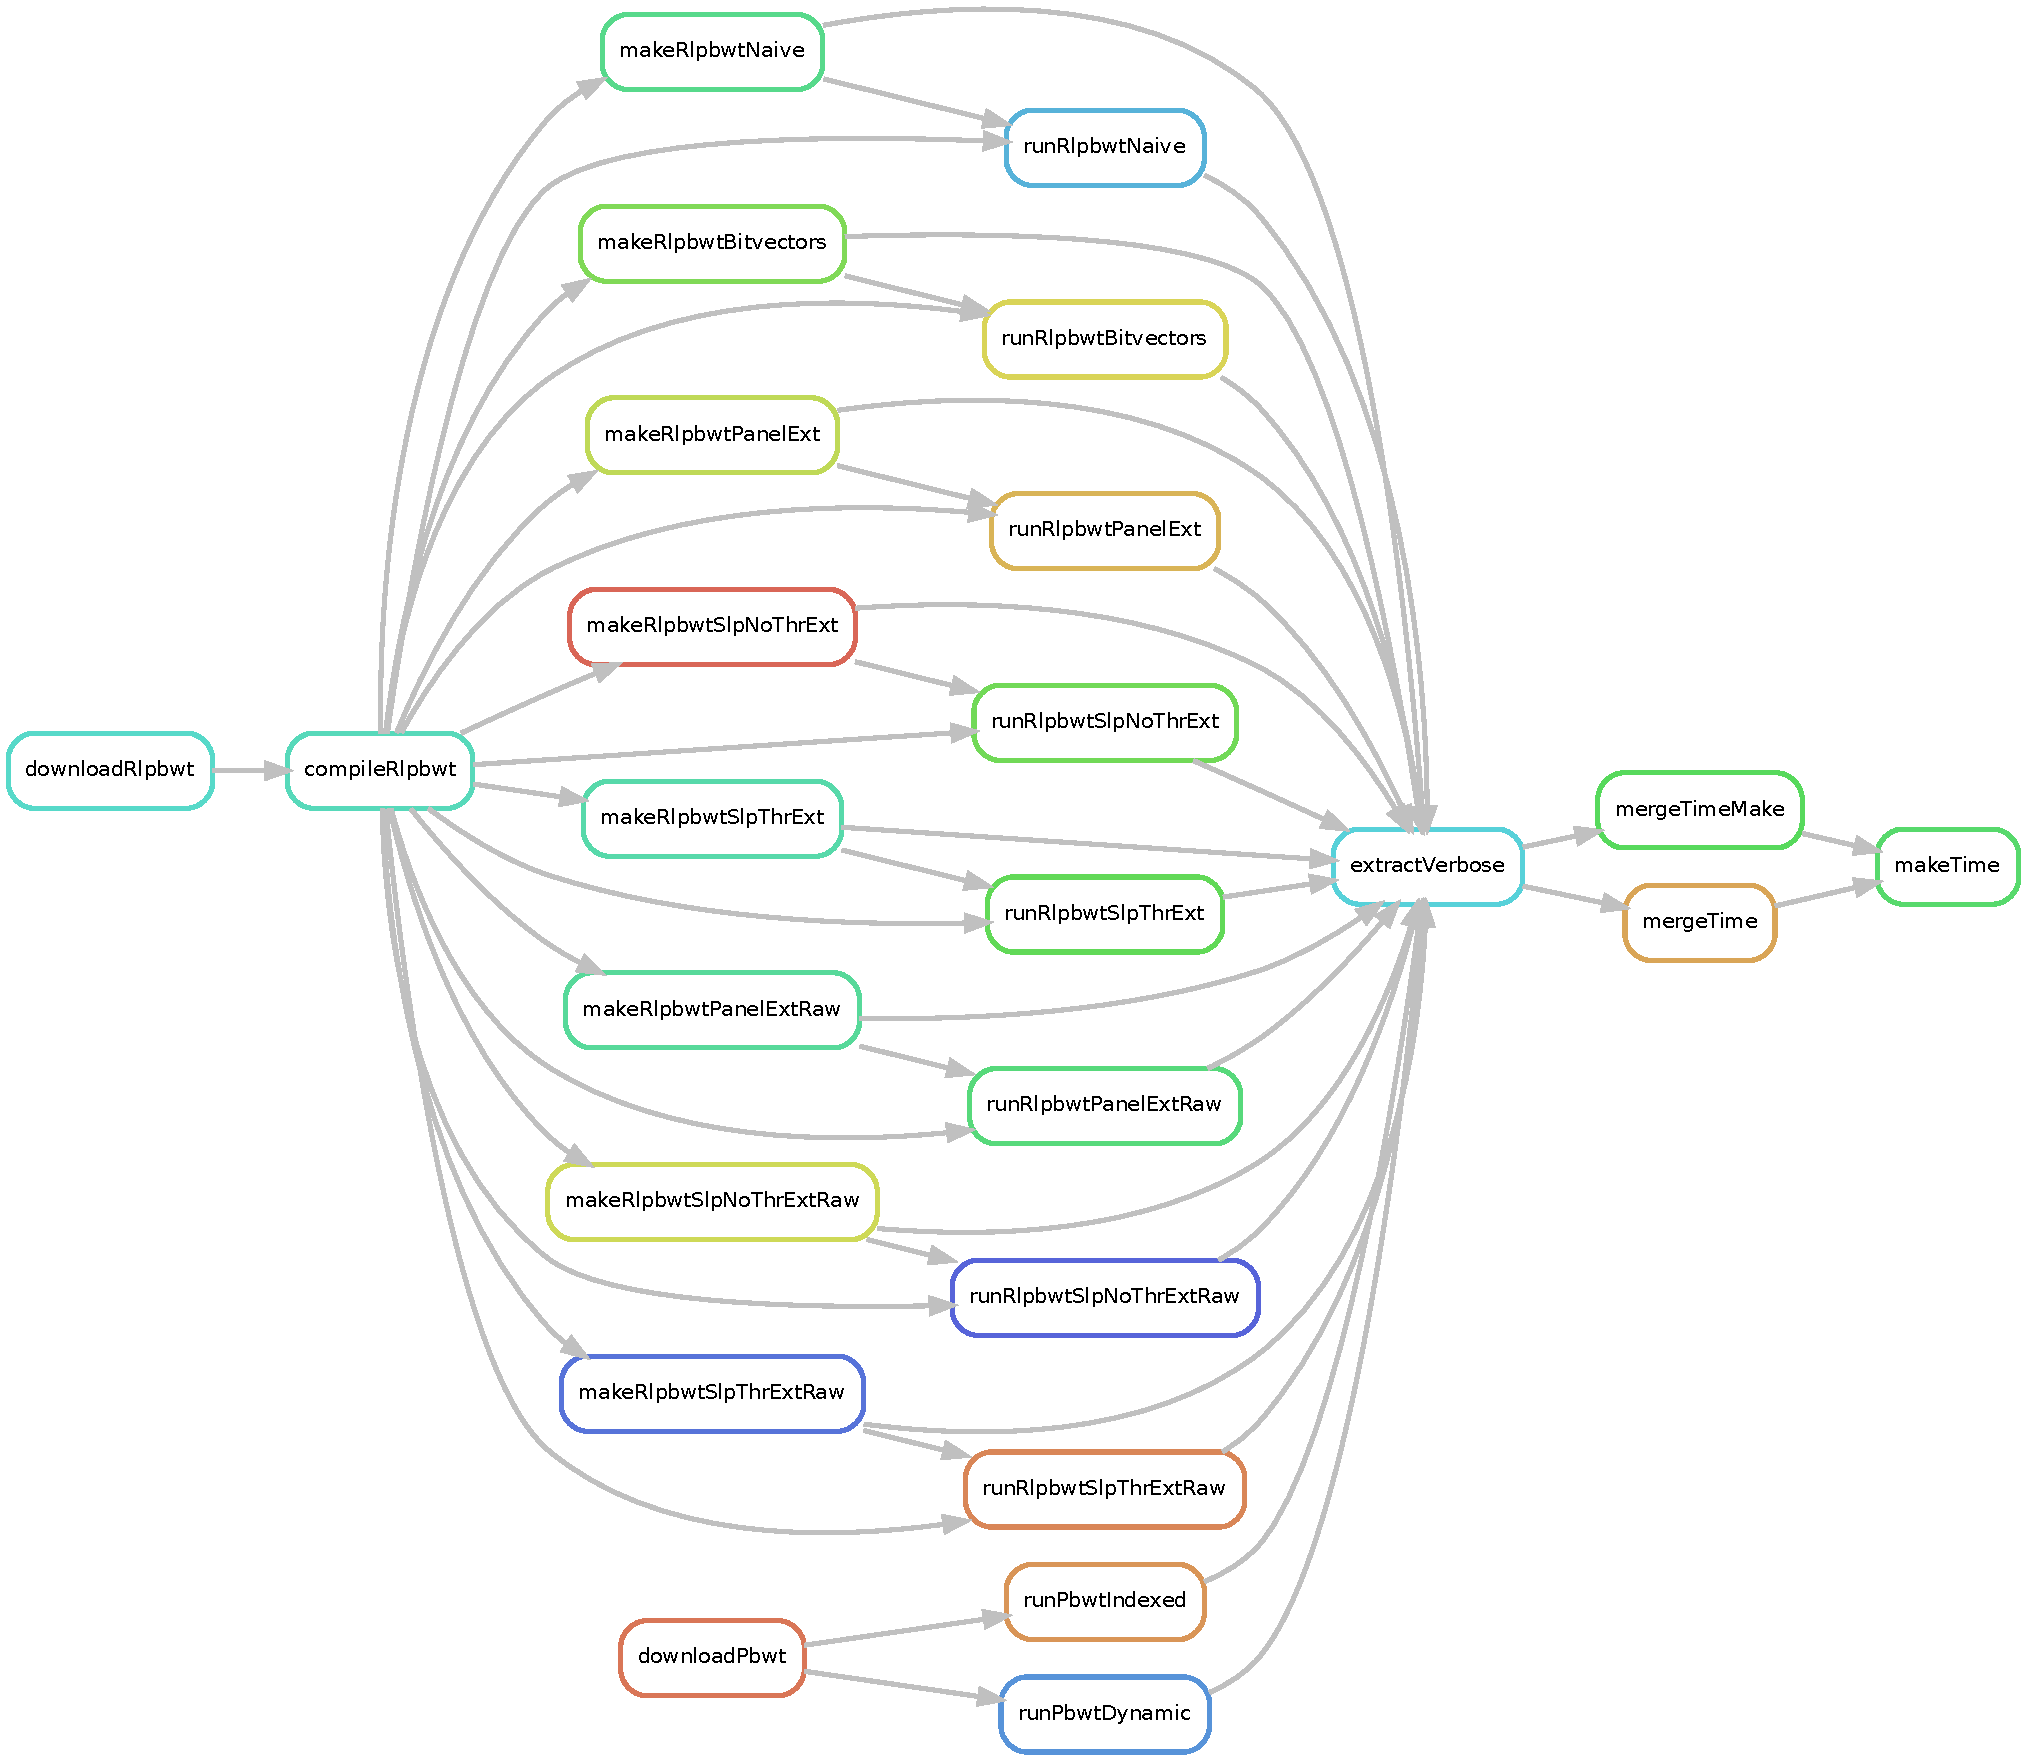
\includegraphics[width=\textwidth]{img/final_dag_r.pdf}
  \vspace{-5mm}
  \caption{Regole usate in Snakemake per la sperimentazione. Si hanno
  il download  dei vari software, la compilazione degli stessi, la produzione
  delle strutture dati,
  il calcolo degli $\SMEM$, l'estrazione dei risultati
  quantitativi e la produzione dei file CSV finali.}
  \label{fig:snake}
\end{figure}
\newline
\textit{La sperimentazione è stata effettuata su una macchina con processore
  Intel Xeon E5-2640 V4 ($2,40$GHz), $756$GB di RAM, $768$GB di swap e
  sistema operativo Ubuntu 20.04.4 LTS. Tale macchina è stata gentilmente messa
  a disposizione dalla \emph{University of Florida}.}
% sezione benchmark
%\section{Ambiente di benchmark}
\subsection{Descrizione input}

% sezione complessità
\section{Confronto tra PBWT e RLPBWT}
Al fine di analizzare i risultati ottenuti si sono confrontate 5 varianti della
\textit{RLPBWT}:
\begin{itemize}
  \item \textit{RLPBWT naive}
  \item \textit{RLPBWT con bitvector}
  \item \textit{RLPBWT con pannello completo e threshold}
  \item \textit{RLPBWT con pannello compresso (SLP) e threshold}
  \item \textit{RLPBWT con pannello compresso (SLP) e LCE query}  
\end{itemize}
Confrontandole con l'implementazione originale dell'algoritmo 5 di Durbin,
nominato \textit{MatchIndexed}. Studiando la repository di Durbin inoltre si è
scoperto l'esistenza di un ulteriore algoritmo, non descritto
formalmente nel paper del 2014 \cite{pbwt} ma solo citato in una tabella, che
considera in un unico panello sia il pannello che l'insieme delle query ed
effettua il matching interno al pannello stesso, calcolando in modo dinamico
l'indicizzazione ad ogni colonna. Nonostante l'algoritmo presenti limiti dal
punto di vista dell'estendibilità ad altre problematiche, avendo che le varianti
della \textit{PBWT} citate in sezione \ref{secpbwt} si basano, nel caso di
\textit{SMEM} 
con aplotipi esterni, sulle idee dell'algoritmo 5, esso risulta essere davvero
molto performante sia dal punto di vista del tempo macchina che della memoria
occupata. A causa di ciò, per completezza, tale algoritmo, chiamato
\textit{MatchDynamic}, è stato incluso nei risultati sperimentali, pur
mancandone una trattazione teorica approfondita.
\subsection{Analisi spaziale}
Lo scopo principale di questa tesi era la riduzione delle informazioni in
memoria necessarie a permette il mapping, quindi in primis si sono valutati i
vari risultati dal punto di vista della memoria.
\subsubsection{Dimensioni dell'SLP}
Prima ancora di affrontare i requisiti
in memoria dell'intera struttura è interessante analizzare le capacità di
compressione che si ha con l'uso degli \textit{SLP}, grazie ai due tool sopra
citati. In figura \ref{fig:slpres1} si può iniziare ad apprezzare l'efficacia di
tale grammatica. Si nota infatti come, per quanto i pannelli siano di dimensione
modesta, hanno un peso che varia in un range di un centinaio di megabytes mentre
gli \textit{SLP} relativi nel centinaio di kilobytes. Si ha infatti:
\begin{table}[H]
  \centering
  \begin{tabular}{c|c|c|c|c}
    \textbf{altezza} & \textbf{larghezza} & \textbf{SLP (\textit{kb})}
    & \textbf{MACs (\textit{kb})} & \textbf{\%}\\
    \hline
    20000 & 4294 & 228.13 & 84050.48 & 0.2714\\
    21000 & 4294 & 238.83 & 88243.83 & 0.2707\\
    22000 & 4294 & 243.04 & 92437.18 & 0.2629\\
    23000 & 4294 & 250.37 & 96630.53 & 0.2591\\
    24000 & 4294 & 272.72 & 100823.87 & 0.2705\\
    25000 & 4294 & 278.22 & 105017.22 & 0.2649\\
    26000 & 4294 & 283.57 & 109210.57 & 0.2597\\
    27000 & 4294 & 288.62 & 113403.92 & 0.2545\\
    28000 & 4294 & 293.85 & 117597.27 & 0.2499\\
    29000 & 4294 & 298.76 & 121790.62 & 0.2453\\
  \end{tabular}
\end{table}
Notando come, per pannelli di grandezza simile, pare si abbia una compressione
proporzionale alla dimensione del pannello.\\
\begin{figure}
  \centering
  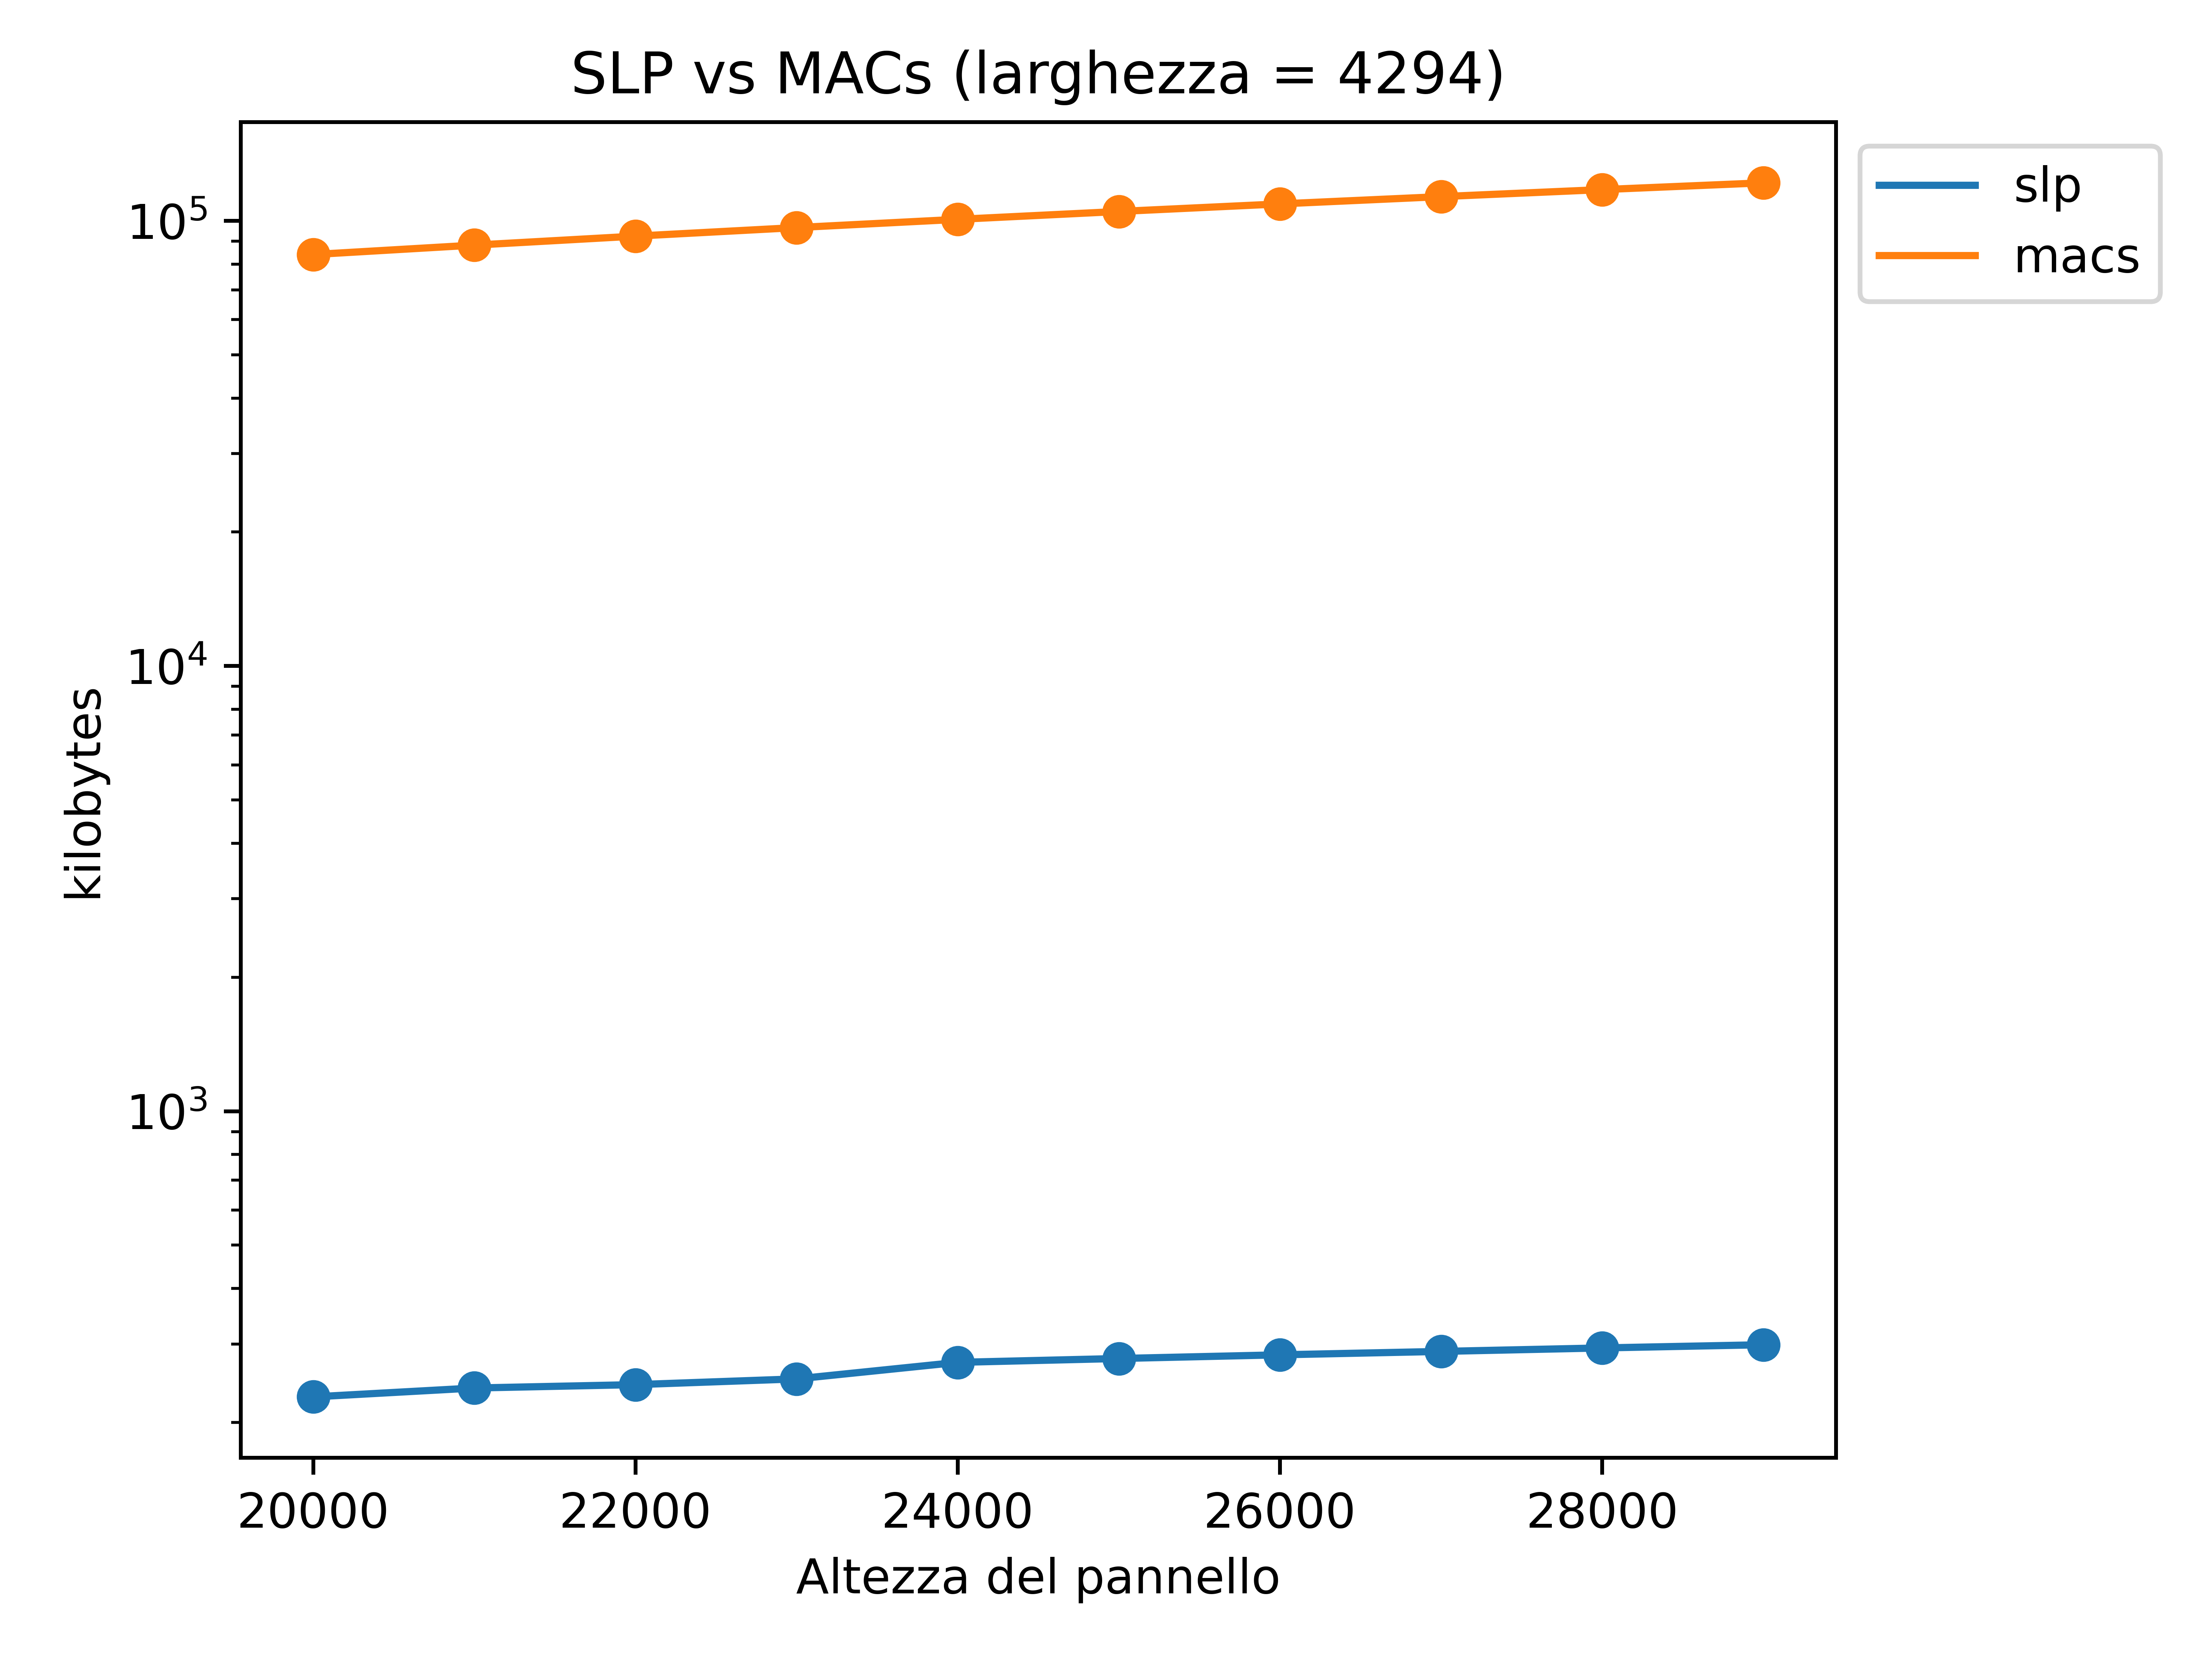
\includegraphics[scale = 0.6]{img/slp_vs_macs.png}
  \caption{Confronto delle dimensioni, espresse in kilobytes, dei pannelli in
    formato \texttt{macs} e dei rispettivi \textit{SLP}. Il grafico è in scala
    logaritmica.}
  \label{fig:slpres1}
\end{figure}
Andando a vedere pannelli molto più grossi si nota come il rateo di
compressione continui essere proporzionale alla dimensione del pannello e,
nonostante il esso cresca di 
dimensione, la grandezza dell'\textit{SLP} resta molto piccola:
\begin{table}[H]
  \centering
  \begin{tabular}{c|c|c|c|c}
    \textbf{altezza} & \textbf{larghezza} & \textbf{SLP (\textit{kb})}
    & \textbf{MACs (\textit{kb})} & \textbf{\%}\\
    \hline
    100000 & 358653 & 14771.0 & 35042963.54 & 0.0422\\
    100000 & 100000 & 9077.88 & 9075120.49 & 0.1\\
    100000 & 46538 & 8017.09 & 4448994.19 & 0.1802\\
  \end{tabular}
\end{table}
Tale risultato è anche apprezzabile in figura \ref{fig:slpres2}.
\begin{figure}
  \centering
  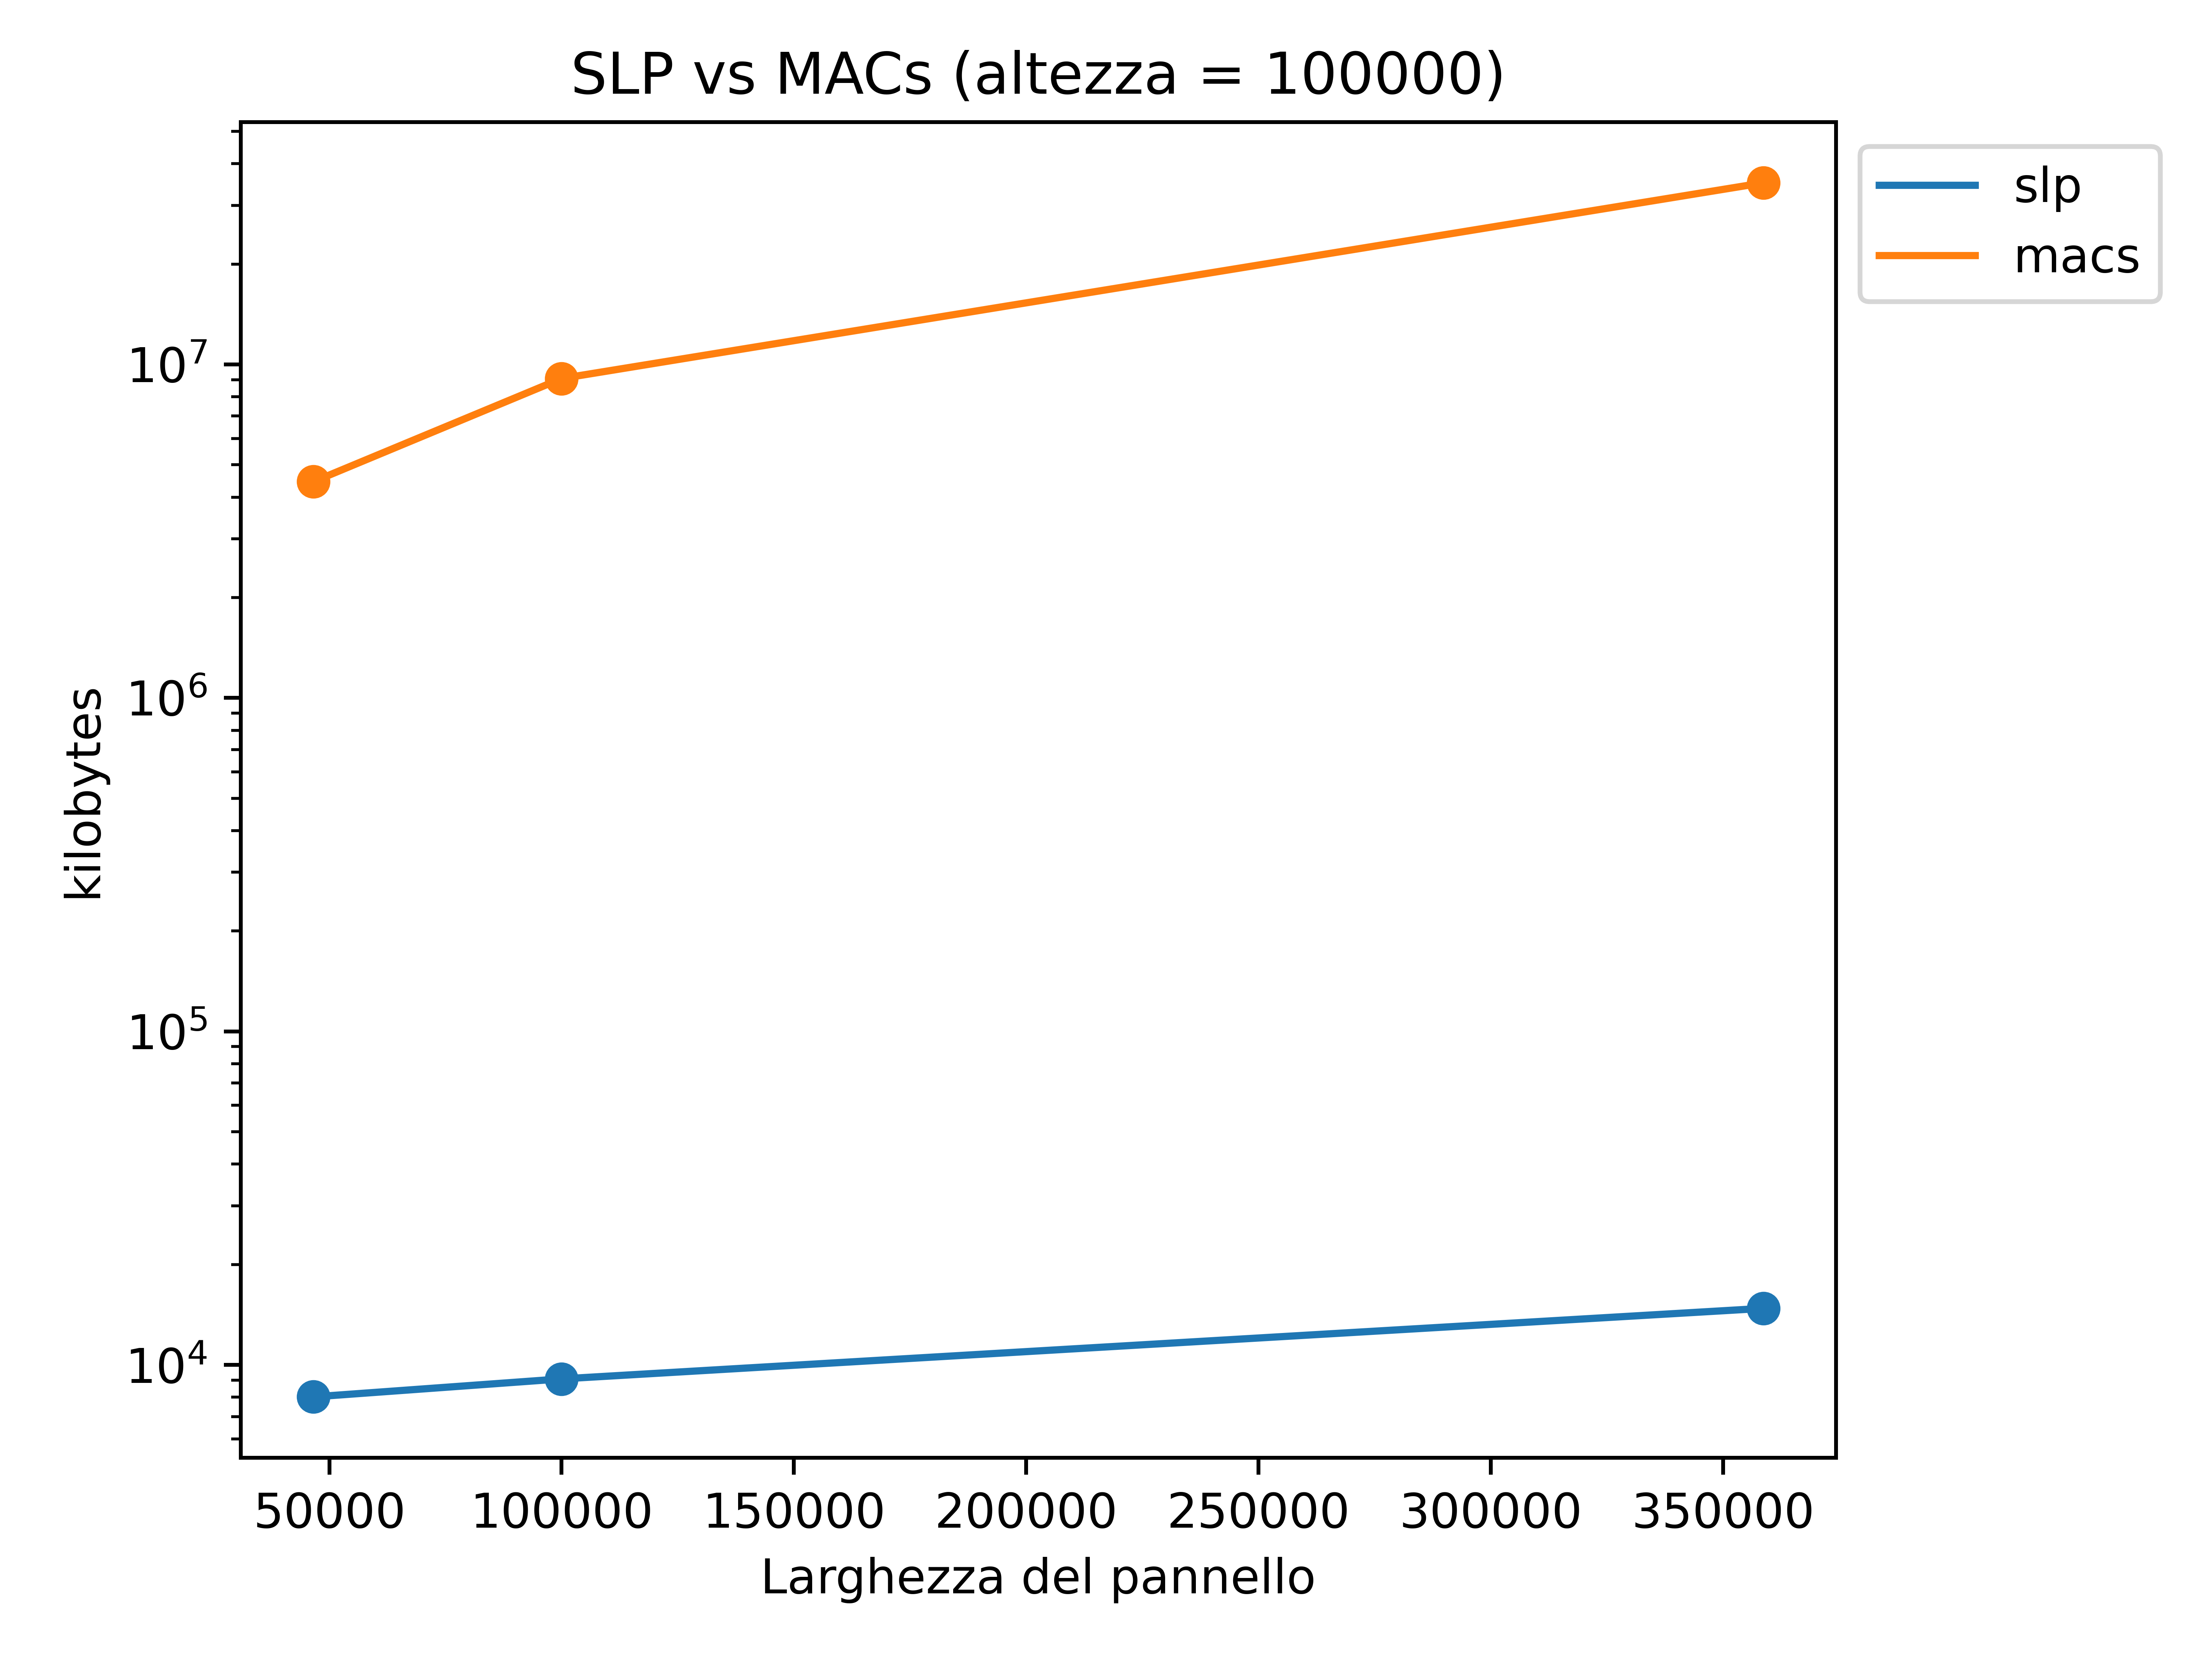
\includegraphics[scale = 0.6]{img/slp_vs_macs2.png}
  \caption{Confronto delle dimensioni, espresse in kilobytes, dei pannelli in
    formato \texttt{macs} e dei rispettivi \textit{SLP}. Il grafico è in scala
    logaritmica.}
  \label{fig:slpres2}
\end{figure}
Il caso estremo, un pannello $100000\times 358653$, occupante in memoria
circa 35gb in formato \texttt{.macs}, viene compresso in circa 15mb. Questo
accade soprattutto in quanto un pannello di soli simboli $\Sigma=\{0,1\}$
contiene molte ripetizioni, permettendo la costruzione di una grammatica,
tramite l'\textit{SLP}, particolarmente ``compatta''.
\subsubsection{Strutture dati}
Si analizzano ora le due strutture dati, confrontando lo spazio richiesto dalle
varie sotto-strutture per effettuare il match con una query esterna, descritte
alle sezioni \ref{secpbwt}, \ref{secrlpbwtnaive}, \ref{secrlpbwtbv} e
\ref{secrlpbwtms}.\\
Si precisa che i dati ora descritti sono stati calcolati nel seguente modo:
\begin{itemize}
  \item per quanto riguarda la \textbf{PBWT}, sfruttando le stime fatte da
  Durbin stesso
  \item per quanto riguarda la \textbf{RLPBWT}, sfruttando le serializzazioni
  ottenute tramite \textit{SDSL}
\end{itemize}
Con un studio al leggero variare del pannello si nota, graficamente in figura
\ref{memcomp1}, come quanto descritto precedentemente venga confermato. Le
informazioni richieste dall'algoritmo 5 di Durbin sono quelle che richiedono
maggior memoria mentre la variante della \textit{RLPBWT} basata su \textit{SLP}
e \textit{LCE query} risulta essere la soluzione migliore tra le varianti della
\textit{RLPBWT}. Bisogna però notare come la soluzione \textit{matchDynamic}
ritrovabile nella repository della \textit{PBWT} risulti essere incredibilmente
più efficace, avendo, secondo Durbin stesso, una richiesta in spazio
proporzionale a $\mathcal{O}(M+N)$. \\
Limitiamo però ora il confronto all'algoritmo 5 di Durbin, in quanto obbiettivo
della tesi. Da un punto di vista di guadagno percentuale in memoria i risultati
sembrano essere interessanti, confrontando tale soluzione con la migliore per la
\textit{RLPBWT}:
\begin{table}[H]
  \centering
  \footnotesize
  \begin{tabular}{c|c|c|c|c}
    \textbf{altezza} & \textbf{larghezza}
    & \textbf{RLPBWT SLP-LCE (\textit{kb})}
    & \textbf{PBWT Indexed (\textit{kb})} & \textbf{\%}\\
    \hline
    20000 & 4294 & 12118.62 & 1090270.65 & 1.1115\\
    21000 & 4294 & 12583.13 & 1144784.18 & 1.0992\\
    22000 & 4294 & 13033.78 & 1199297.71 & 1.0868\\
    23000 & 4294 & 13487.57 & 1253811.24 & 1.0757\\
    24000 & 4294 & 13954.44 & 1308324.78 & 1.0666\\
    25000 & 4294 & 14419.27 & 1362838.31 & 1.058\\
    26000 & 4294 & 14867.82 & 1417351.84 & 1.049\\
    27000 & 4294 & 15316.41 & 1471865.37 & 1.0406\\
    28000 & 4294 & 15765.41 & 1526378.9 & 1.0329\\
    29000 & 4294 & 16214.09 & 1580892.44 & 1.0256\\
  \end{tabular}
\end{table}
Provando in modo quantitativo l'efficacia in memoria della soluzione ultima
proposta in questa tesi.

% \begin{table}[H]
%   \centering
%   \tiny
%   \begin{tabular}{c|c|c|c|c|c|c|c|c}
%     \textbf{Altezza} & \textbf{Larghezza} & \textbf{Naive}
%     & \textbf{Bitvector} & \textbf{Pannello}
%     & \textbf{SLP-Thr} & \textbf{SLP-LCE} & \textbf{Indexed}&
%                                                               \textbf{Dynamic}\\
%     \hline
%     20000 & 4294 & 116872.34 & 118842.8 & 22956.56 & 12422.86 & 12118.62
%                                                      & 1090270.65 & 20004.19\\
%     21000 & 4294 & 122717.92 & 124689.87 & 23954.83 & 12884.39 & 12583.13
%                                                        & 1144784.18 & 21004.19\\
%     22000 & 4294 & 128541.43 & 130509.84 & 24911.04 & 13337.4 & 13033.78
%                                                        & 1199297.71 & 22004.19\\
%     23000 & 4294 & 134383.15 & 136347.63 & 25900.01 & 13789.62 & 13487.57
%                                                        & 1253811.24 & 23004.19\\
%     24000 & 4294 & 140197.73 & 142157.96 & 26853.09 & 14239.5 & 13954.44
%                                                        & 1308324.78 & 24004.19\\
%     25000 & 4294 & 146047.34 & 148014.12 & 27855.43 & 14705.09 & 14419.27
%                                                        & 1362838.31 & 25004.19\\
%     26000 & 4294 & 151872.56 & 153834.89 & 28841.15 & 15154.06 & 14867.82
%                                                        & 1417351.84 & 26004.19\\
%     27000 & 4294 & 157711.32 & 159670.04 & 29793.47 & 15603.17 & 15316.41
%                                                        & 1471865.37 & 27004.19\\
%     28000 & 4294 & 163536.4 & 165489.58 & 30779.6 & 16052.56 & 15765.41
%                                                        & 1526378.9 & 28004.19\\
%     29000 & 4294 & 169381.28 & 171331.14 & 31765.37 & 16501.58 & 16214.09
%                                                        & 1580892.44 & 29004.19\\
    
%   \end{tabular}
% \end{table}
\begin{figure}
  \centering
  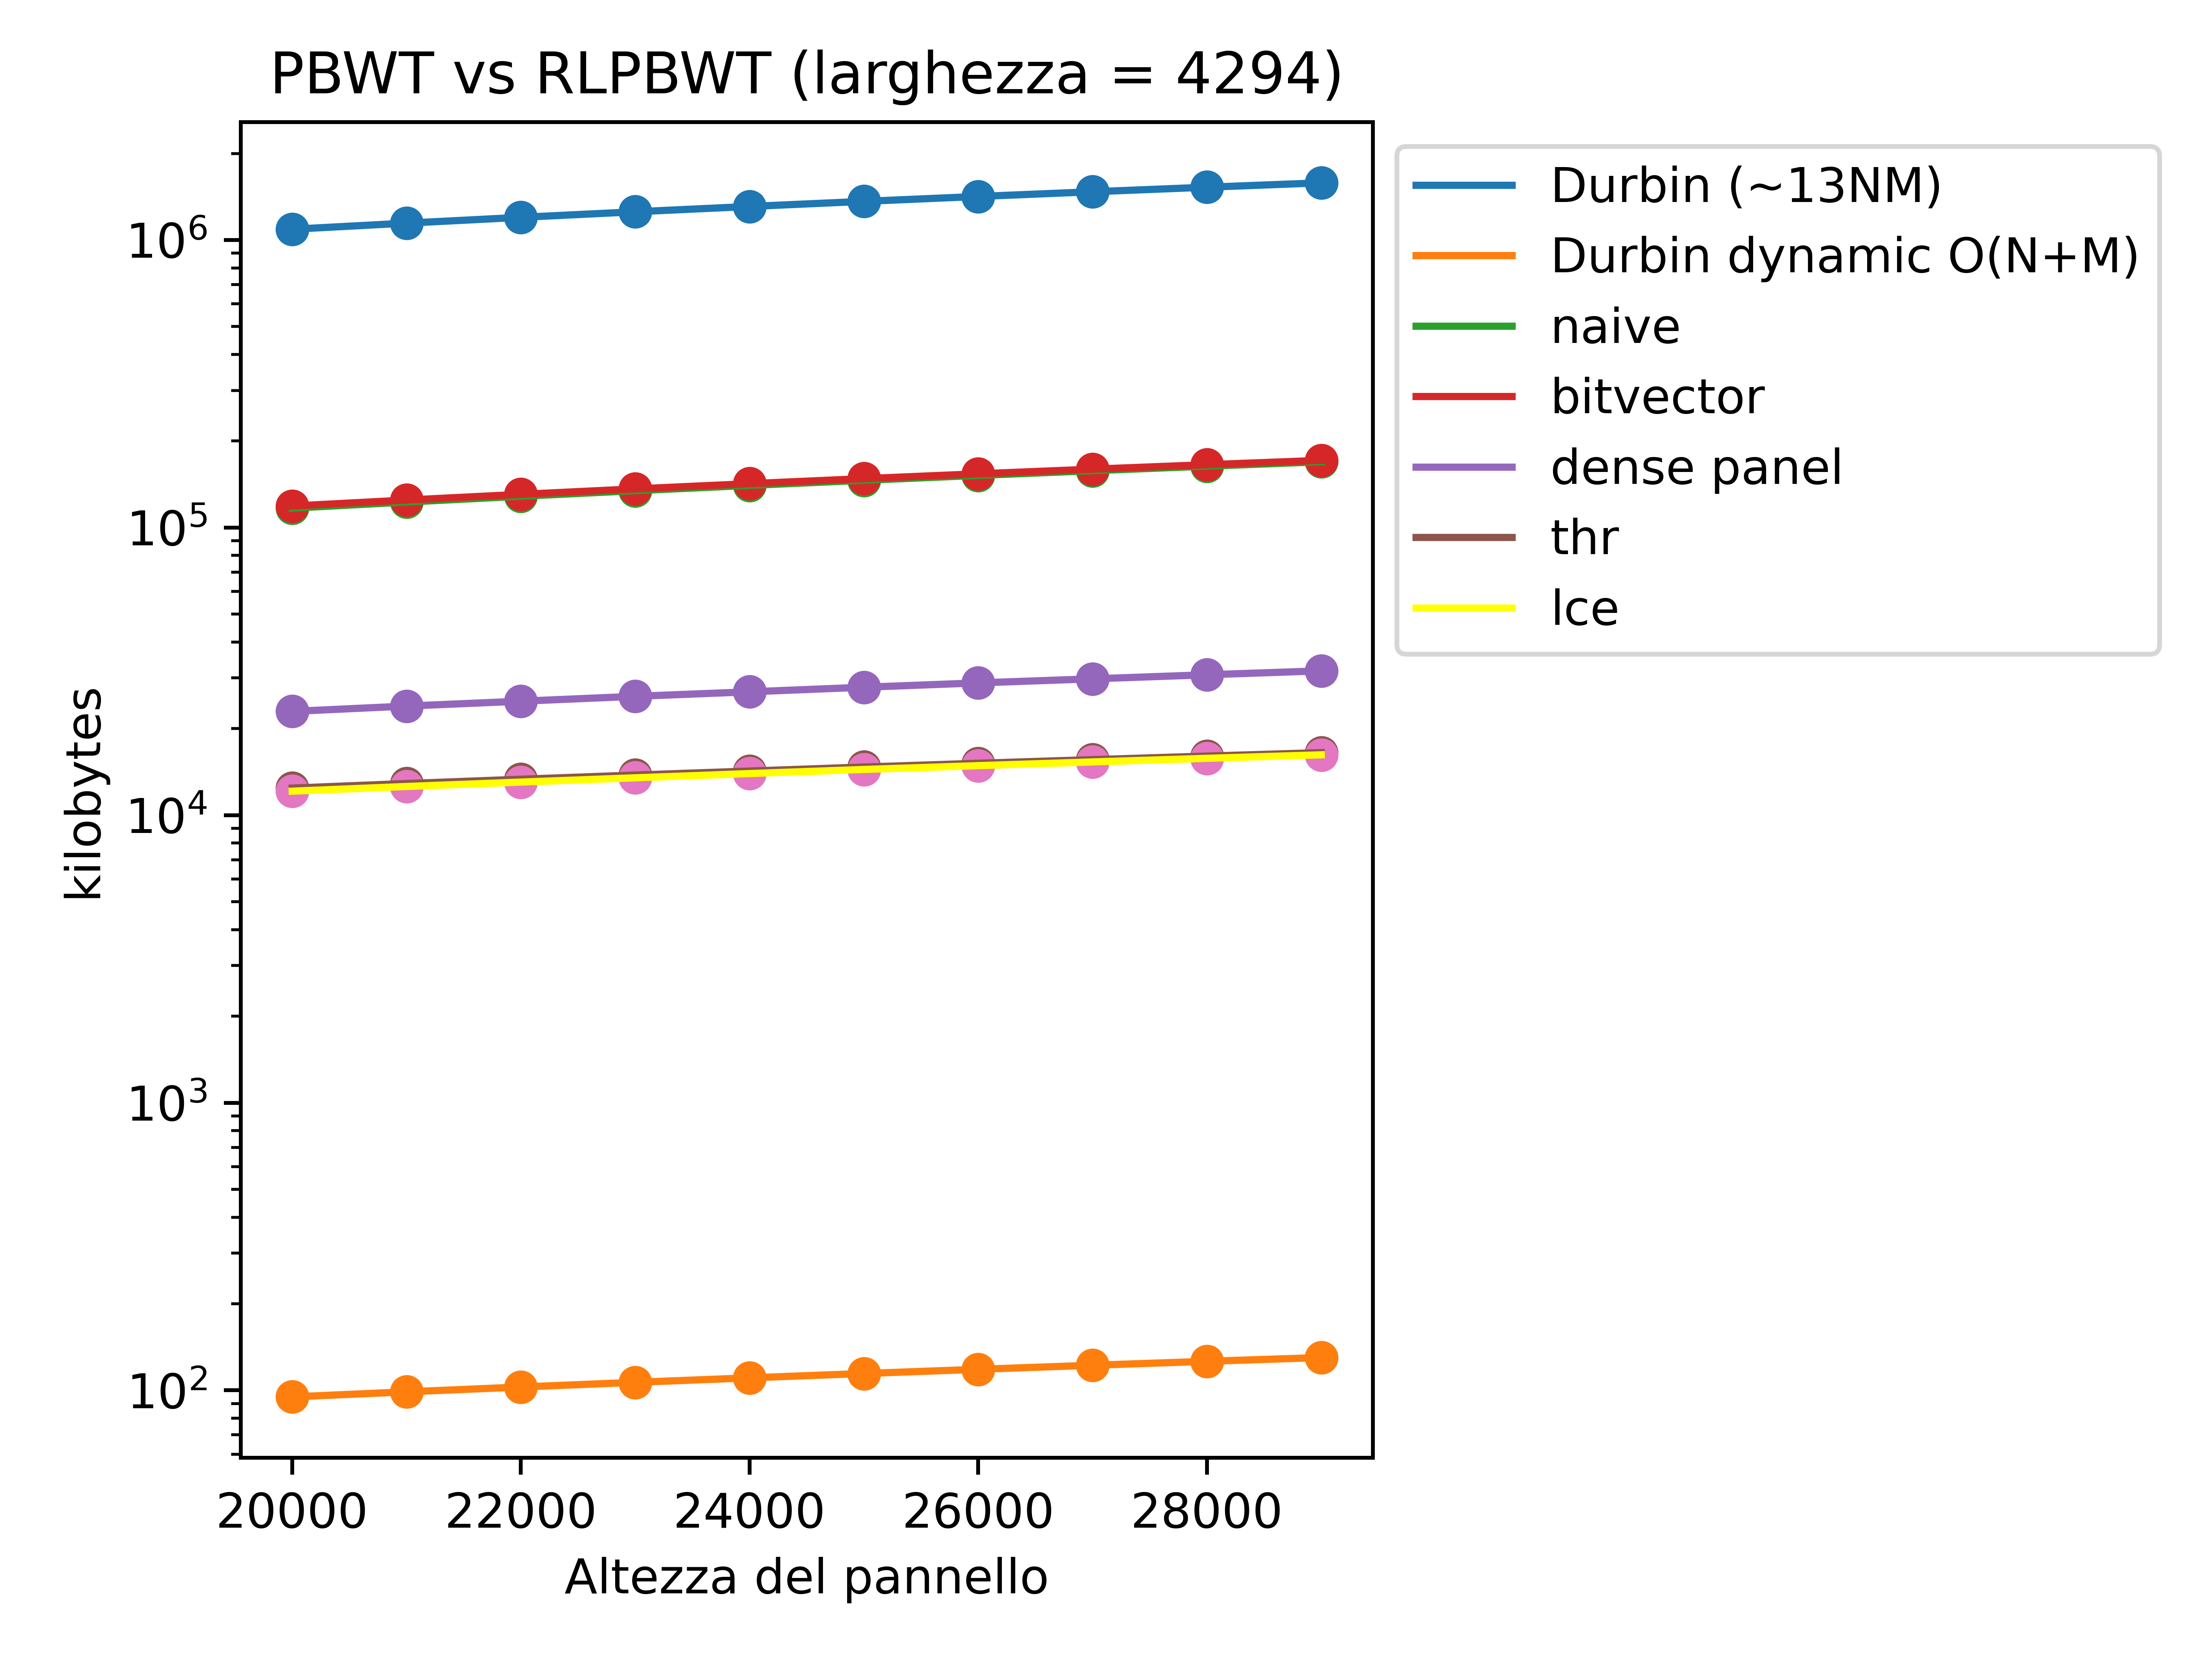
\includegraphics[scale = 0.6]{img/pbwt_vs_rlpbwt_dyn.png}
  \caption{Confronto dello spazio in memoria, in kilobytes, richiesto dalle
    varie strutture dati.} 
  \label{memcomp1}
\end{figure}
\subsection{Analisi temporale}
Bisogna infine considerare i tempi di esecuzione per il pattern matching con un
pannello di query. Dal punto di vista della \textit{RLPBWT} bisogna considerare
in primis due aspetti:
\begin{itemize}
  \item avere meno informazione in memoria comporta molto probabilmente, a
  parità di risultati, tempi maggiori
  \item l'uso di strutture dati succinte ed eventualmente dell'\textit{SLP}
  comporta costi dal punto di vista temporale. Come anticipato in sezione
  \ref{bvsec}, le operazioni sugli sparse bitvector non sono tutte i tempo
  costante e, come invece anticipato in sezione \ref{slpsec}, gli \textit{SLP}
  non garantiscono \textit{random access} in tempo costante e questo, per quanto
  poi l'algoritmo di estensione sia efficiente, si ripercuote anche sul calcolo
  delle \textit{LCE query}
\end{itemize}
Questa premessa fa capire come ci si aspettasse che i tempi fossero maggiori con
la \textit{RLPBWT}, in ogni sua variante, rispetto all'algoritmo 5 di Durbin.
Parlando invece dell'algoritmo \textit{matchDynamic} si ha che, per quanto
asintoticamente presenti la stessa complessità dell'algoritmo 5, ovvero
$\mathcal{O}(N(M+Q))$, con $Q$ numero di query, esso risulta incredibilmente più
performante. \\
Alcuni risultati sono visualizzabili in figura \ref{fig:1000} e \ref{fig:10000},
dove si possono osservare sia i tempi che lo spazio richiesto. Anche la completa
esecuzione quindi conferma come l'algoritmo 5 sia incredibilmente esoso dal
punto di vista dello spazio richiesto, pur avendo ottime performance
temporali. Dal punto di vista invece delle varianti della \textit{RLPBWT} si
nota come:
\begin{itemize}
  \item la \textit{RLPBWT naive}, priva dell'uso dei bitvector e
  dell'\textit{SLP}, risulti essere la più performante, anche se, si ricordi,
  non permette di identificare quali righe stiano effettivamente matchando ma
  solo quante
  \item la \textit{RLPBWT con bitvector}, avente lo stesso limite della variante
  naive, presenta anche maggiori costi in termini di memoria di quest'ultima,
  avendo anch'essa ancora l'\textit{LCP array} completo ma anche tutte le
  informazioni memorizzate in bitvector, che aumentano, come anticipato, i tempi
  di calcolo. La chiave delle varianti che sfruttano
  le \textit{matching statistics} è infatti quella di non avere l'\textit{array
    LCP} in memoria, una delle cause principali dell'aumento di spazio richiesto
  \item le tre varianti basate sulle \textit{matching statistics} hanno spazio
  occupato pressoché uguale, anche se si può percepire, nei due casi studiati,
  come il tenere l'intero pannello in forma di bitvector, all'aumentare della
  grandezza dello stesso, comporti molta più memoria degli \textit{SLP}. Dal
  punto di vista temporale, inoltre, anche se si ha \textit{random access} in
  tempo costante, all'aumentare del pannello, il numero di accessi allo stesso
  comporta forti costi in termini di tempo macchina. Questi
  ultimi, infatti, come già visto occupano pochissima memoria anche con pannelli
  molto estesi. Dal punto di vista temporale si rileva come la variante basata
  su \textit{SLP} e \textit{threshold} richieda molto più tempo. Si nota che ciò
  accade a causa di due fattori:
  \begin{itemize}
    \item il continuo accesso all'\textit{SLP} per calcolare $MS[i].len$
    \item l'eventuale accesso all'\textit{SLP} per disambiguare le threshold a
    fine run
  \end{itemize}
  Tra le tre quindi la variante con \textit{SLP} e \textit{LCE query},
  all'aumentare della grandezza del pannello, risulta essere la soluzione
  migliore
\end{itemize}

\begin{figure}
  \centering
  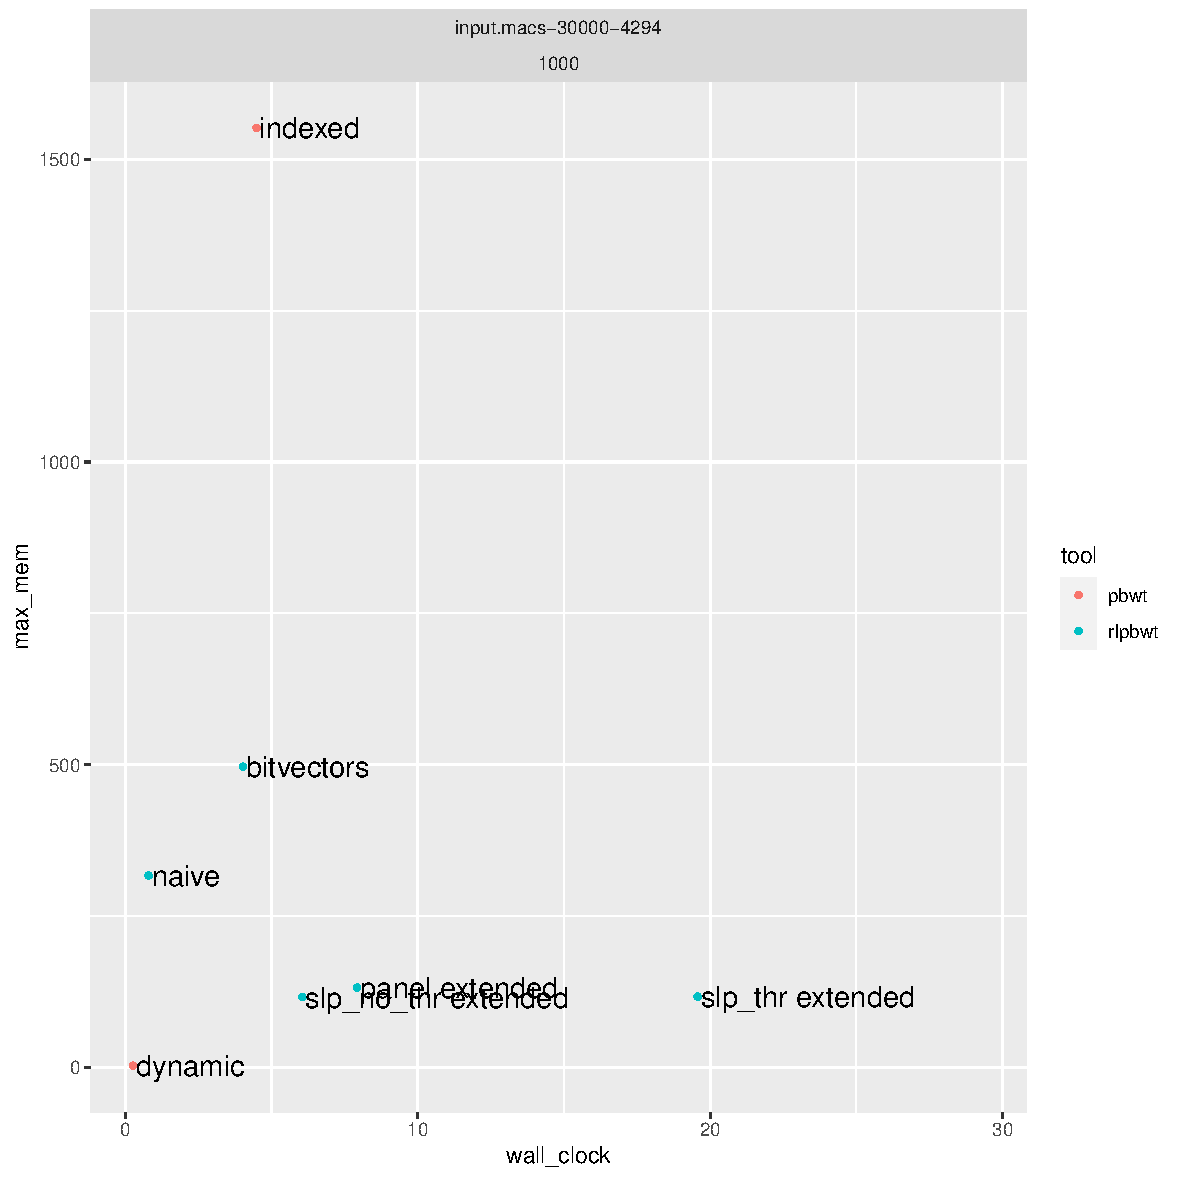
\includegraphics[scale = 0.35]{img/time_vs_mem_1000.pdf}
  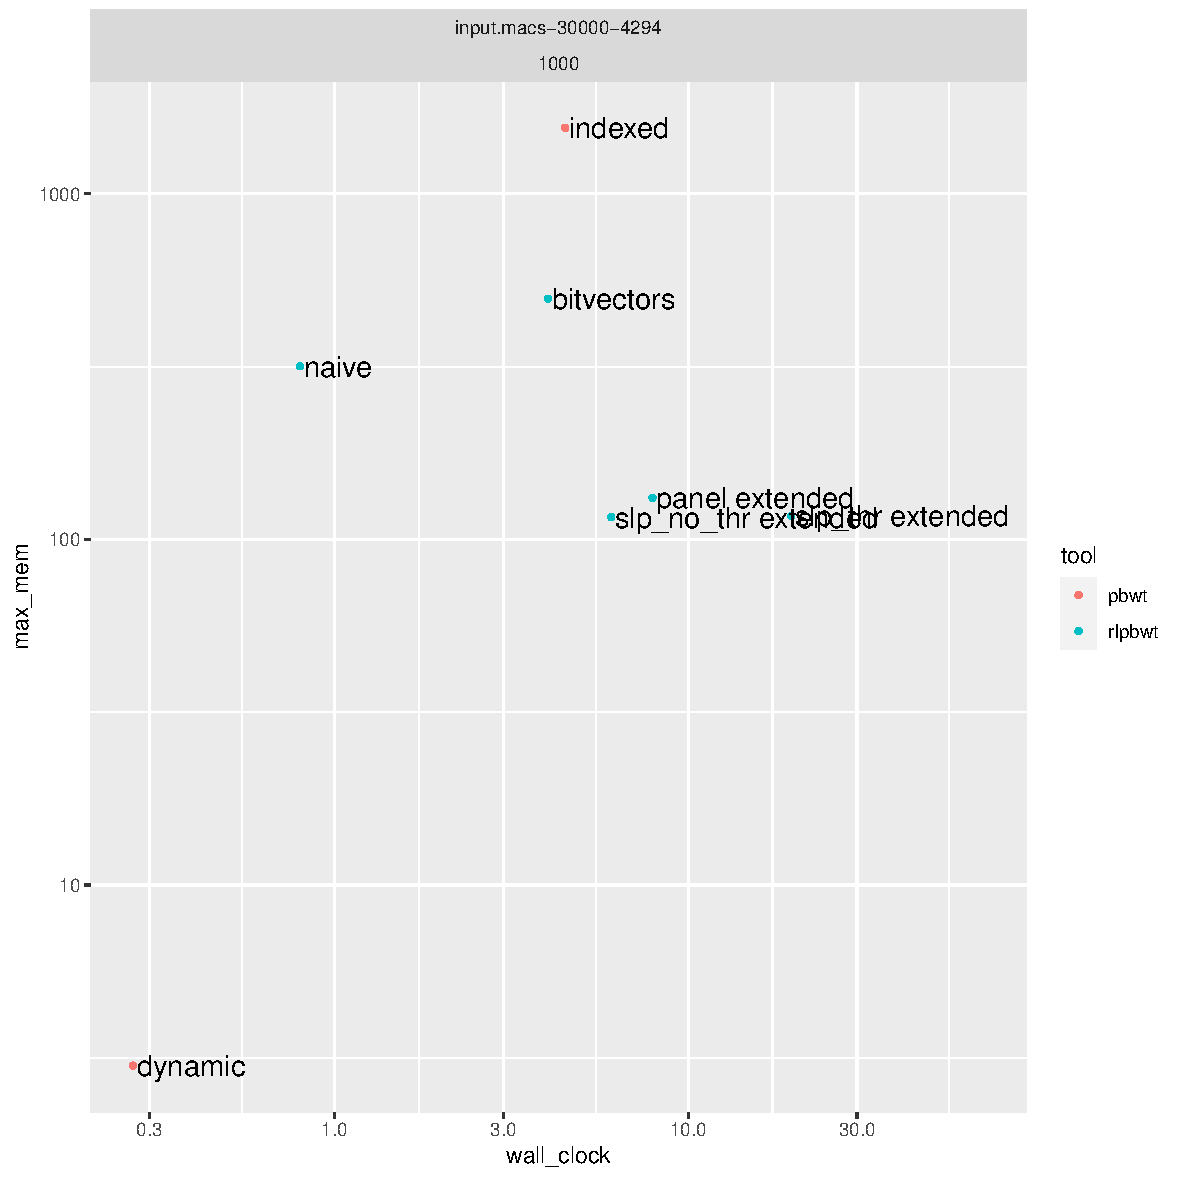
\includegraphics[scale = 0.35]{img/time_vs_mem-loglog_1000.pdf}
  \caption{Esecuzione dei vari algoritmi di match su un pannello
    $29000\times 4294$ e 1000 query.  Il grafico a destra è in scala
    logaritmica. }
  \label{fig:1000}
\end{figure}

\begin{figure}
  \centering
  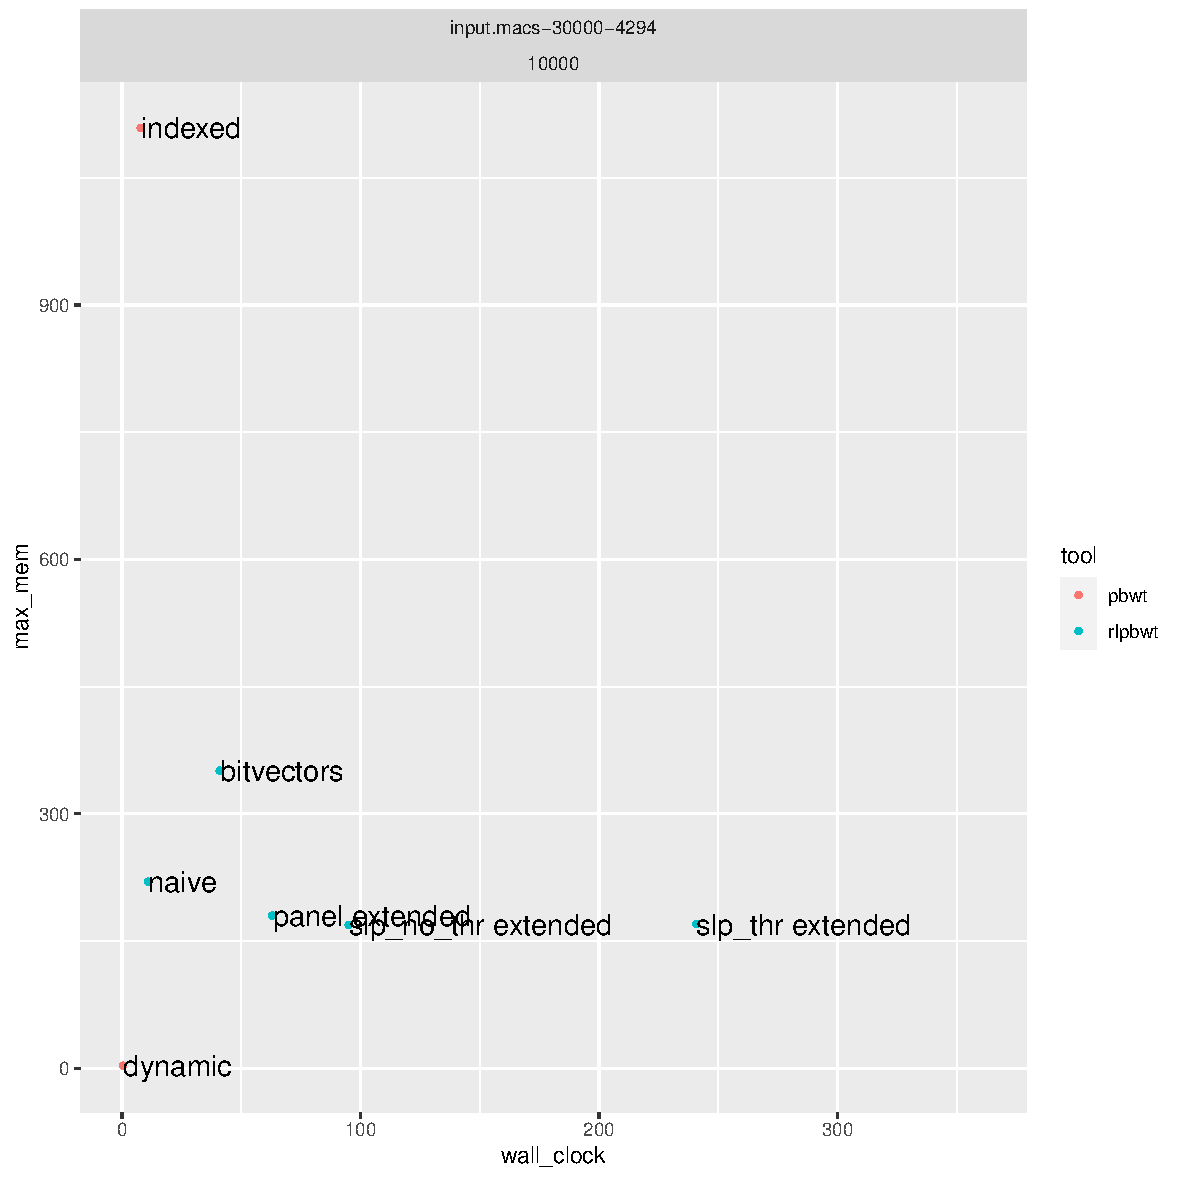
\includegraphics[scale = 0.35]{img/time_vs_mem_10000.pdf}
  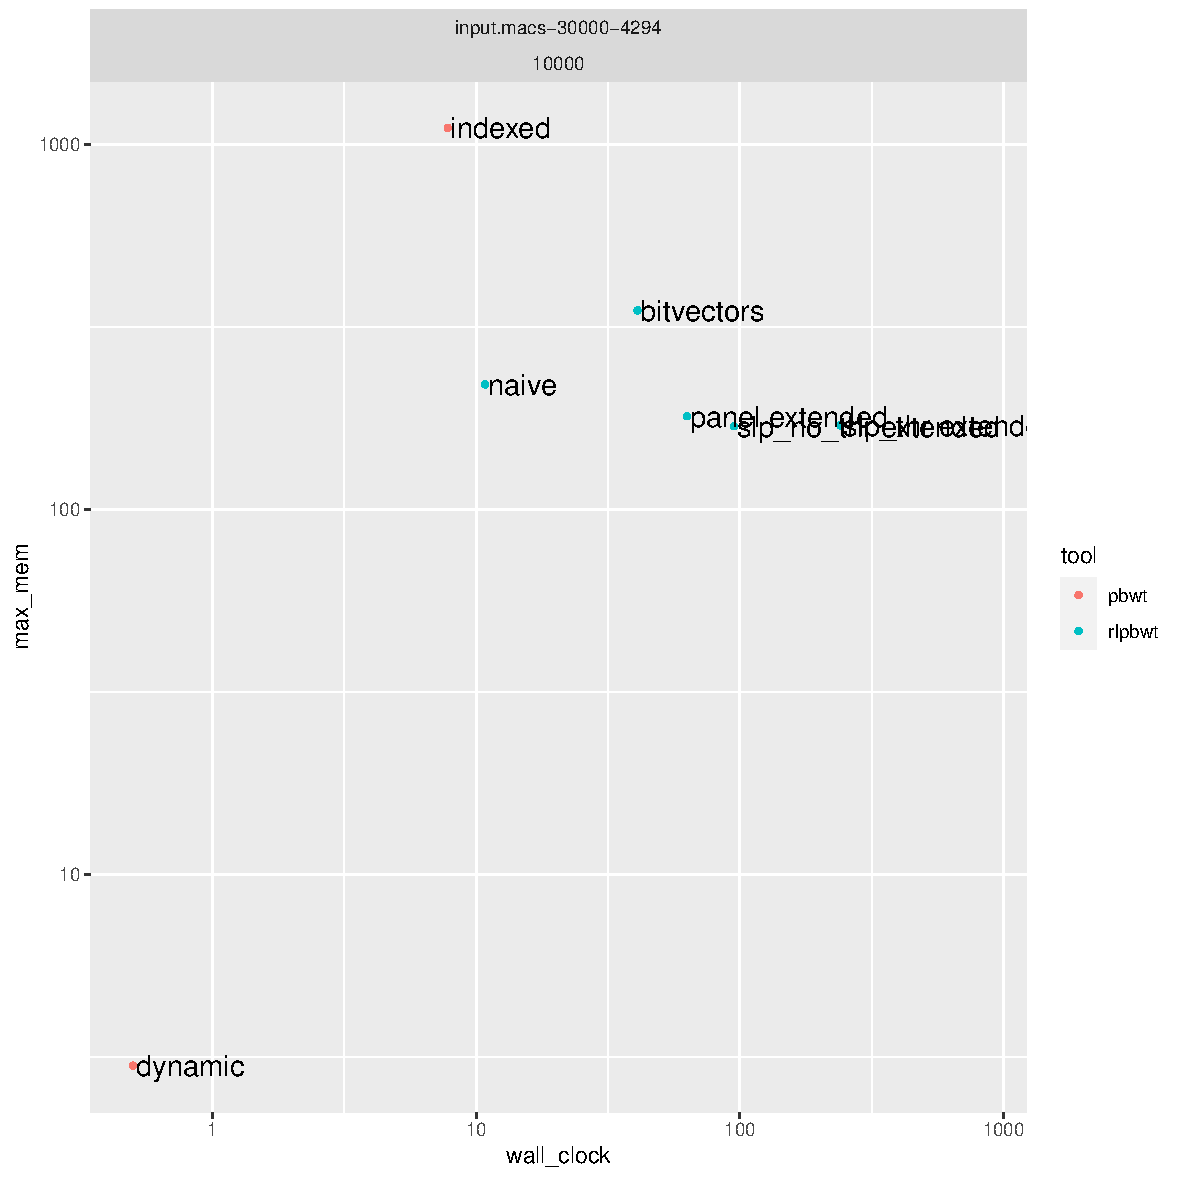
\includegraphics[scale = 0.35]{img/time_vs_mem-loglog_10000.pdf}
  \caption{Esecuzione dei vari algoritmi di match su un pannello
    $20000\times 4294$ e 10000 query. Il grafico a destra è in scala
    logaritmica. }
  \label{fig:10000}
\end{figure}
Per completezza, in figura \ref{fig:bigres}, si riportano anche i risultati in
tempo 
e spazio di una sperimentazione su un pannello di grandi dimensioni:
$70000\times 46538$ con $30000$ query. Sono riportati anche i risultati delle
tre varianti basate su \textit{matching statistics} senza l'estensione dei match
tramite le \textbf{funzioni} $\boldsymbol \varphi$ e
$\boldsymbol\varphi^{\mathbf{-1}}$. Si può notare come la struttura dati aggiuntiva
non comporti praticamente alcuna differenza sostanziale sia in termini di
memoria che di tempo di calcolo. In merito agli altri risultati si ha che
seguono tutti il trend già descritto negli esempi precedenti. In particolare si
nota che:
\begin{itemize}
  \item l'algoritmo 5 di Durbin ha una richiesta di memoria davvero molto
  grande, parlando di circa 40.75 gb di memoria richiesta
  \item l'algoritmo \textit{matchDynamic} di Durbin risulta essere migliore sia
  dal punto di vista dello spazio richiesto che del tempo d'esecuzione. Parlando
  di tempi, infatti, l'intera esecuzione richiede $\sim 22$s, contro i $\sim
  411$ dell'algoritmo \textit{matchIndexed} e i $\sim 1824$ della
  \textit{RLPBWT} con \textit{SLP} e \textit{LCE query}
  \item la variante \textit{RLPBWT} con \textit{SLP} e \textit{threshold}, per
  le problematiche già descritte richiede un tempo d'esecuzione importante,
  parlando di circa 2 ore di esecuzione
\end{itemize}
\begin{figure}
  \centering
  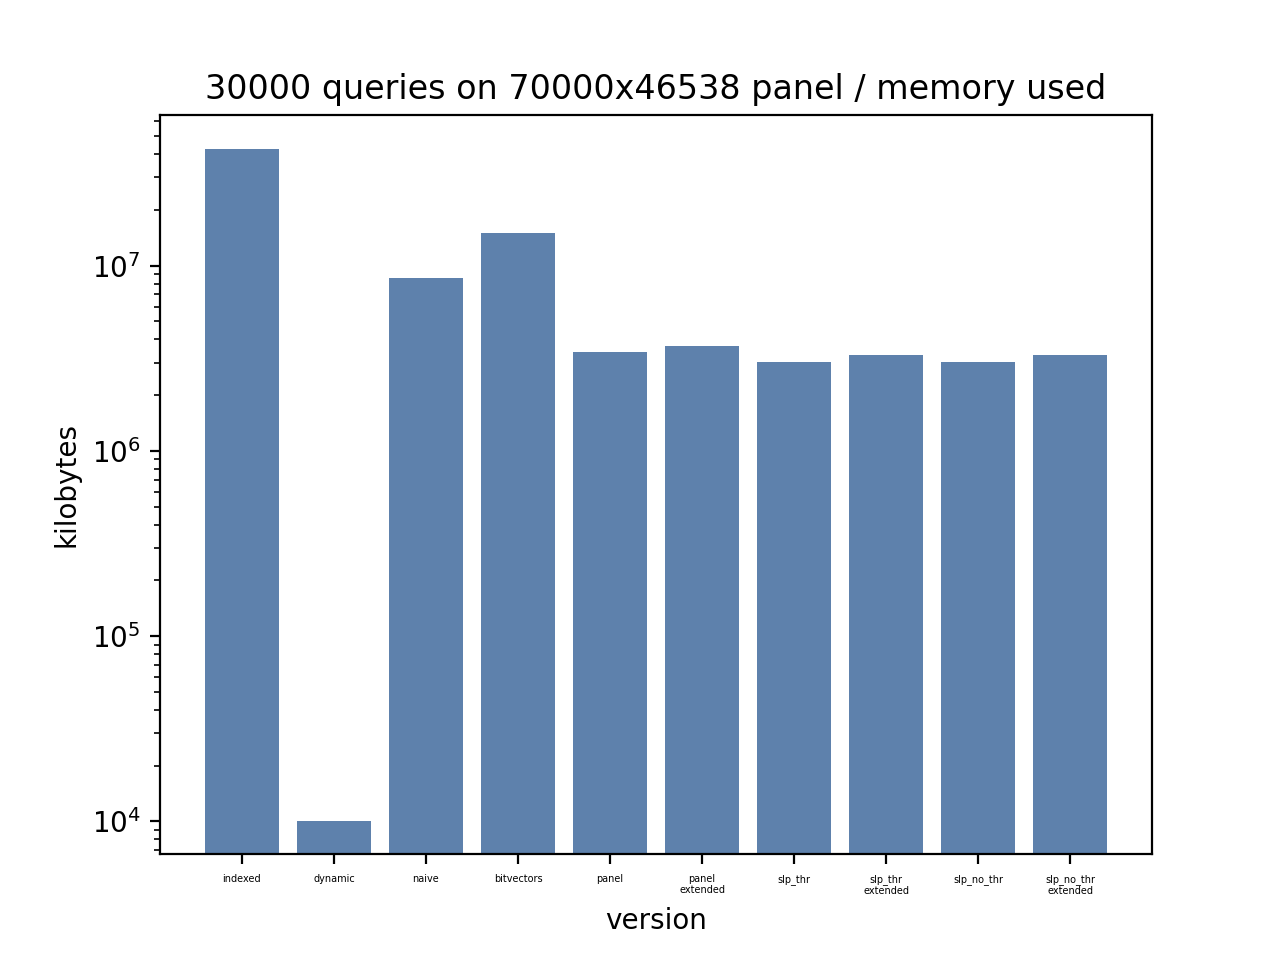
\includegraphics[scale = 0.4]{img/mem.png}
  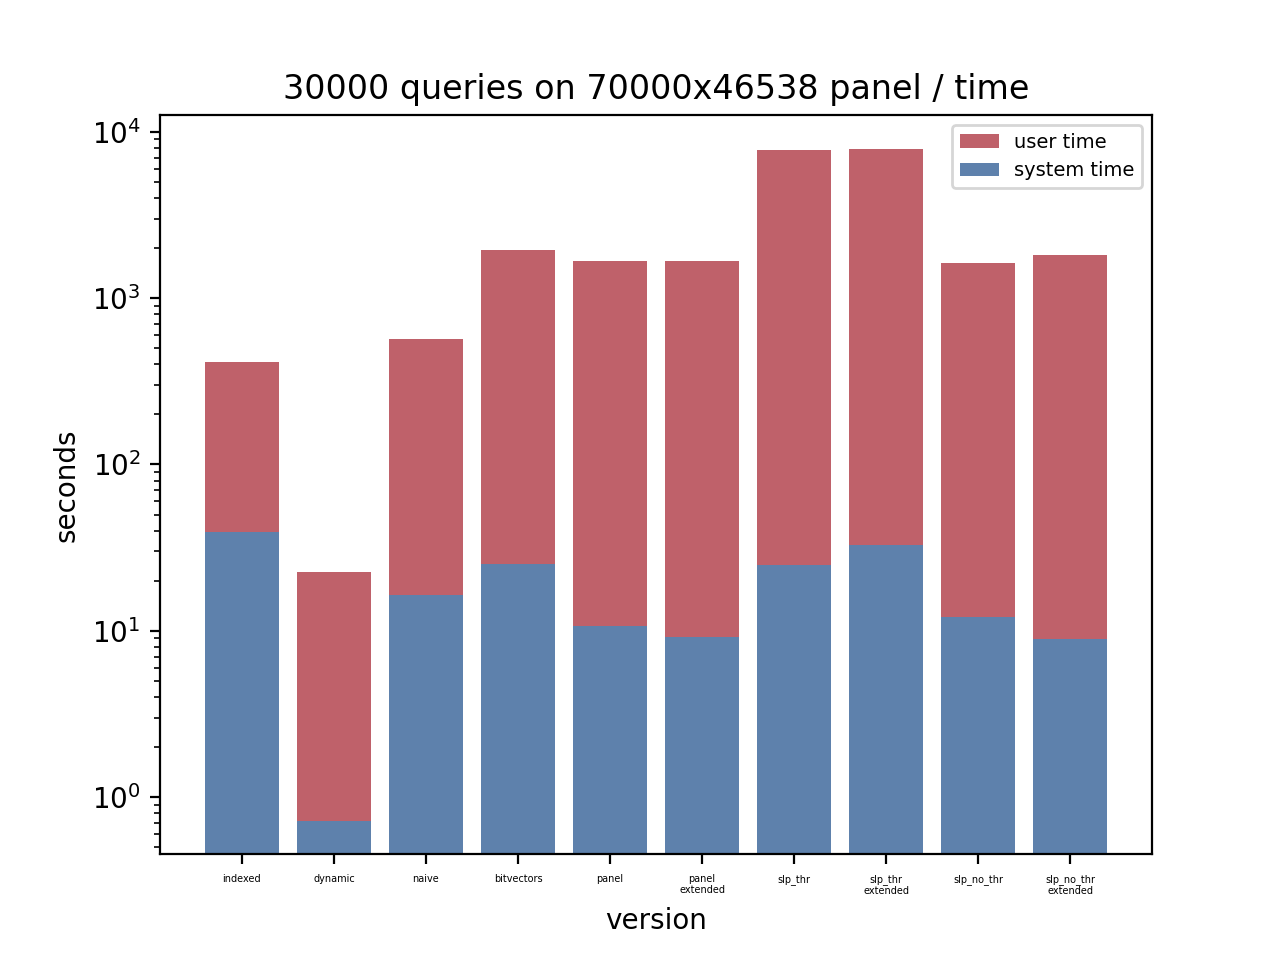
\includegraphics[scale = 0.4]{img/time.png}
  \caption{Risultati, in scala logaritmica, dell'esecuzione dei vari algoritmi
    su un pannello di grosse dimensioni. Si noti che, quantitativamente, la
    variante \textit{matchIndexed} richieda $42736132$ kb di memoria mentre la
    \textit{RLPBWT} con \textit{SLP} e \textit{LCE query} solo $3286424$ kb,
    richiedendo quindi appena il 7\% di memoria richiesta dall'algoritmo 5 di
    Durbin. Infine, per quanto la scala logaritmica renda impercettibile tale
    differenza, la variante \textit{RLPBWT} con pannello richiede $3695968$ kb,
    quindi circa $380$ mb in più della soluzione basata sull'uso
    dell'\textit{SLP}. } 
  \label{fig:bigres}
\end{figure}




\chapter{Conclusioni}
\label{conchap}
Fissato l'iniziale obbiettivo di risolvere le problematiche relative alla
memoria richiesta dall'algoritmo 5 di Durbin, l'implementazione della
\textbf{RLPBWT}, nel dettaglio basata sull'uso dei \textit{SLP} e \textit{LCE
  query}, ha riportato risultati molto incoraggianti. Come descritto nel
capitolo \ref{reschap}, la quantità di memoria richiesta risulta essere
incredibilmente inferiore. D'altro canto l'algoritmo \textit{matchDynamic} di
Durbin, per quanto non approfondito nell'articolo del 2014 \cite{pbwt}, risulta
essere ancor meno esoso di risorse, nonché incredibilmente più veloce dal punto
di vista dei tempi di calcolo. Lo svantaggio di questo algoritmo è che i
risultati sono prodotti in ``ordine sparso'' e, giudicando la letteratura degli
ultimi anni le cui trattazioni si basano sempre sull'algoritmo 5, che non sembra
essere facilmente riadattabile per la risoluzione di altri task.\\
Si possono comunque rilevare alcune possibili migliorie in merito
all'implementazione attuale della \textit{RLPBWT}:
\begin{itemize}
  \item si potrebbe pensare ad un metodo per gestire in modo efficiente lo
  studio di più query contemporaneamente, migliorando i tempi di calcolo
  complessivi
  \item studiare eventuali ottimizzazioni per l'algoritmo di mapping e per le
  strutture dati richieste, studiando, ad esempio, se sia possibile tenere in
  memoria un solo bitvector $uv_k$ che funzioni in modo similare a quanto si era
  inizialmente pensato per la \textit{RLPBWT naive}
  \item migliorare il sistema di serializzazione. Allo stato attuale l'intera
  struttura viene serializzata e caricata in modo completo. Studiare una
  strategia efficiente per caricare, di volta in volta, in memoria solo la
  colonna necessaria ad un dato passo di computazione o comunque un sottoinsieme
  di colonne
\end{itemize}
Nonostante queste possibili migliorie la qualità dei risultati è sufficiente per
stabilire che una variante \textit{run-length encoded} della \textit{PBWT}, alla
stregua di quanto analizzato negli ultimi anni sulla \textit{RLBWT} con
\textit{MONI} \cite{moni} e \textit{PHONI} \cite{phoni}, sia possibile e possa
permettere, nel prossimo futuro, la memorizzazione compatta delle informazioni
necessarie allo studio di grandi pannelli di aplotipi. In un futuro in cui le
tecnologie di sequencing produrranno sempre più dati da sempre più individui,
avere a disposizione strutture dati efficienti dal punto di vista della
memorizzazione permetterà uno studio sempre più approfondito dei dati stessi,
nei campi dei \textit{genome-wide association studies}, della \textit{medicina
  personalizzata} etc\ldots 
% sezione sviluppi
\section{Sviluppi futuri}
Ovviamente, questa prima implementazione completa della $\RLPBWT$,
declinata nelle possibili strutture composte, non è da
considerarsi come un punto di arrivo. Come accaduto per la $\PBWT$,
infatti, si potranno sviluppare nuove strutture dati basate su di essa per la
gestione di pannelli di varia natura. Principalmente si può pensare a due casi,
già anticipati nella sezione \ref{secpbwt}:
\begin{itemize}
  \item lo studio di pannelli multiallelici, ovvero costruiti su un alfabeto
  $\Sigma$ arbitrario e non limitato ai simboli $\sigma=0$ e $\sigma=1$
  \item lo studio di pannelli con dati mancanti, ovvero pannelli costruiti
  da dati reali che possono contenere siti, per certi
  individui, per i quali non si ha certezza in merito all'allele
\end{itemize}
Inoltre, allo stato attuale, la struttura dati è stata sviluppata per permettere
unicamente il calcolo degli $\SMEM$ con un aplotipo esterno. Anche in
questo caso, quindi, si potrebbe avere lo sviluppo di nuovi algoritmi che
rispondano a task diversi, come, ad esempio, il calcolo degli $\SMEM$ interni al
panello, il 
calcolo dei cosiddetti \textit{blocchi}, o anche il calcolo di tutti i match con
un aplotipo 
esterno di lunghezza maggiore ad una fissata o che includano un numero stabilito
di sequenze di aplotipi nel panello.
\dc{Serve definire i blocchi?}
\paragraph{RLPBWT multiallelica.}
Per quanto i pannelli di aplotipi, prodotti dal sequencing del genoma umano.
raramente presentino siti multiallelici, si ha una presenza stimata, al momento,
di circa il 2\% di siti triallelici \cite{tri}. Inoltre, all'aumentare della
disponibilità di dati genomici, si ha in letteratura la propensione a credere
che tale percentuale di siti sia non solo sottostimata (evidenziando che sia
stimato 
circa un terzo dei reali siti triallelici) ma anche destinata a
crescere in modo non lineare rispetto al numero di individui sequenziati
\cite{tri2}. Inoltre, molte specie, soprattutto vegetali, sono già riconosciute
essere poliploidi. Una struttura dati efficiente in memoria, in grado di
gestire pannelli costruiti su un alfabeto arbitrario, risulterà necessaria nel
breve futuro.\\
Ipotizzando un possibile funzionamento della $\RLPBWT$
multiallelica ($\MRLPBWT$), si può pensare ad una soluzione molto
simile a quanto visto per la $\RLBWT$. Infatti, per ogni colonna, si
potrebbero memorizzare:
\begin{itemize}
  \item una stringa che memorizzi quale simbolo corrisponda ad una certa run,
  non potendo sfruttare l'alternanza di simboli vista nel caso binario
  \item una rivisitazione delle strutture necessarie al mapping, tenendo in
  memoria vettori di bitvector sparsi o di intvector compressi, al fine di poter
  computare la funzione $w(i,\sigma)$ anche nel caso multiallelico. Si segnala
  che si attende un inversione di 
  tendenza in termini di memoria, avendo che, in tal caso, l'uso di intvector
  compressi potrebbe rivelarsi meno efficiente dell'uso dei bitvector sparsi,
  anche con pochi sample
  \item un riadattamento del calcolo dell'array delle matching statistics 
\end{itemize}
In merito allo spazio richiesto e ai tempi di calcolo bisognerà considerare la
grandezza dell'alfabeto su cui è costruito il pannello, che ci si aspetta,
fortunatamente, 
inferiore a $10$ nella maggioranza dei casi di studio biologico.\\
Quindi, nonostante, allo stato dell'arte, ci siano pochissimi studi in merito,
si ritiene 
possibile generalizzare, in modo computazionalmente efficiente, la
$\RLPBWT$ anche a questa casistica. 
\paragraph{RLPBWT con dati mancanti.}
La maggior parte delle soluzioni attualmente sviluppate sono basate su una forte
assunzione: i dati in input sono corretti e senza dati mancanti. Ovviamente,
limitandosi a studiare pannelli simulati corretti in una fase di
preprocessing, si rischia di limitare la capacità di inferenza dai pannelli
stessi.\\ 
Come anticipato alla sezione \ref{secpbwt}, si sono iniziate a sviluppare
estensioni della $\PBWT$ che ammettano wildcard, ovvero simboli nel
pannello che possono assumere qualsiasi valore dell'alfabeto $\Sigma$, su cui è
costruito il pannello stesso.\\
Uno degli sviluppi futuri sarebbe quindi quello di generalizzare la
$\RLPBWT$, ma anche l'eventuale $\MRLPBWT$, per la gestione di dati
mancanti nel pannello. Inoltre, si potrebbero sviluppare algoritmi in grado di
gestire le wildcard anche all'interno delle query stesse.\\
Sempre in via ipotetica, l'uso di algoritmi parametrici (ma anche
di algoritmi approssimati), adattati al
funzionamento della $\RLPBWT$, potrebbero portare a soluzioni interessanti
per la gestione di pannelli reali non preprocessati.
\paragraph{K-SMEM.}
Come anticipato, oltre che variare le caratteristiche del pannello in analisi,
si possono studiare anche algoritmi per risolvere nuovi task con la
$\RLPBWT$.\\ 
Di recente, Gagie \cite{kmems} ha proposto un articolo in cui dimostra come
la $\RLBWT$, implementata in MONI \cite{moni}, sia già predisposta al
calcolo dei $\KMEM$, ovvero $\MEM$, tra sottostringhe di un
pattern e un testo, che occorrono esattamente $k$ volte nel testo stesso.\\
In merito alla $\RLPBWT$, si potrebbe adattare l'idea di Gagie al calcolo
dei $\KSMEM$, tra sottostringhe dell'aplotipo query e il pannello, che
comportino $\SMEM$ con esattamente $k$ righe del pannello stesso. La
correlazione tra la $\RLBWT$ e la $\RLPBWT$ 
porta a pensare che tale problema sia risolvibile anche con la nuova definizione
di matching statistics presentata in questa tesi.\\
Nulla è stato sviluppato al momento ma si ritiene questo
un'interessante sviluppo futuro in quanto permetterebbe studi statistici, molto
comuni nei GWAS, in merito alla presenza di sottostringhe di un
aplotipo esterno all'interno di un pannello di aplotipi.\\
\\
\\
\textit{La tematica della \emph{pangenomica} è innovativa e il numero di
problemi aperti è incredibilmente grande. I dati aumentano sempre di più e gli
studi informatici devono evolversi per ``stare al passo'' con questa mole
d'informazioni. Gli \emph{sviluppi futuri} sono, da diversi punti di vista,
anche imprevedibili. Risulta quindi difficile elencare, in modo completo, le
possibilità future dietro questa branca della bioinformatica e dell'algoritmica
sperimentale.}
\dc{Frase conclusiva da modificare fortemente}
% LocalWords:  preprocessing

%% BIBLIOGRAFIA
% \addcontentsline{toc}{chapter}{Bibliografia e sitografia}
% \printbibliography[title={Bibliografia e sitografia}]
%\addcontentsline{toc}{chapter}{Bibliografia}
\addcontentsline{toc}{chapter}{Riferimenti}
\bibliographystyle{unsrt}
\bibliography{thesis}
\dc{Sistemare tutte le citazione coi DOI}
\appendix
% \chapter{Tabelle}
% % tabella dello spazio occupato dalle varianti dei bit vector
\begin{table}[H]
  \small
  \centering
  \caption{Stime dello spazio occupato per la memorizzazione di alcune varianti
    di \textit{bit vector}. Si 
    assume un bit vector di lunghezza $n$ con un numero di bit posti pari a
    1 (o $\top$) pari a $m$. $K$ indica un valore costante.} 
  \begin{tabular}{c|c}
    \textbf{Variante} & \textbf{Spazio occupato}\\
    \hline\xrowht{15pt}
    \textit{Plain bitvector} & $64\big\lceil\frac{n}{64}+1\big\rceil$\\
    \hline\xrowht{15pt}
    \textit{Interleaved bitvector} & $\approx n\left(1+\frac{64}{K}\right)$\\
    \hline\xrowht{15pt}
    \textit{$H_0$-compressed bitvector} & $\approx\big\lceil\log\binom{n}{m}\big\rceil$\\
    \hline\xrowht{15pt}
    \textit{Sparse bitvector} & $\approx m\left(2+\log\frac{n}{m}\right)$\\
  \end{tabular}
  \label{tab:bvspace}
\end{table}

% tabella relativa ai costi della funzione rank dei bitvector
\begin{table}[H]
  \small
  \centering
  \caption{Complessità temporali stimate della \textit{funzione rank} per alcune
    varianti di \textit{bit 
      vector}, con la quantità di bit aggiuntivi richiesta. Si assume un bit
    vector di lunghezza $n$, con un numero di bit 
    posti pari a 1 (o $\top$) pari a $m$, e un numero $k$ di valori prima della
    posizione richiesta.} 
  \begin{tabular}{c|c|c}
    \textbf{Variante} & \textbf{Bit aggiuntivi} & \textbf{Complessità
                                                  temporale}\\ 
    \hline\xrowht{15pt}
    \textit{Plain bitvector} & $0.0625\cdot n$ & $\mathcal{O}(1)$\\
    \hline\xrowht{15pt}
    \textit{Interleaved bitvector} & $128$ & $\mathcal{O}(1)$\\
    \hline\xrowht{15pt}
    \textit{$H_0$-compressed bitvector} & $80$ & $\mathcal{O}(k)$\\
    \hline\xrowht{15pt}
    \textit{Sparse bitvector} & $64$ & $\mathcal{O}\left(\log\frac{n}{m}\right)$\\ 
  \end{tabular}
  \label{tab:rank}
\end{table}

% tabella relativa ai costi della funzione select dei bitvector
\begin{table}[H]
  \small
  \centering
  \caption{Complessità temporali stimate della \textit{funzione select} per
    alcune varianti di \textit{bit 
      vector}, con la quantità di bit aggiuntivi richiesta. Si assume un bit
    vector di lunghezza $n$, con un numero di bit 
    posti pari a 1 (o $\top$) pari a $m$.} 
  \begin{tabular}{c|c|c}
    \textbf{Variante} & \textbf{Bit aggiuntivi} & \textbf{Complessità
                                                  temporale}\\ 
    \hline\xrowht{15pt}
    \textit{Plain bitvector} & $\leq 0.2\cdot n$ & $\mathcal{O}(1)$\\
    \hline\xrowht{15pt}
    \textit{Interleaved bitvector} & $64$ & $\mathcal{O}(\log n)$\\
    \hline\xrowht{15pt}
    \textit{$H_0$-compressed bitvector} & $64$ & $\mathcal{O}(\log n)$\\
    \hline\xrowht{15pt}
    \textit{Sparse bitvector} & $64$ & $\mathcal{O}(1)$\\ 
  \end{tabular}
  \label{tab:rank}
\end{table}
\chapter{Algoritmi}
% TODO COSTRUZIONE NAIVE e UVTRICK NAIVE
\begin{algorithm}
  \scriptsize
  \begin{algorithmic}[1]
    \Function{build}{$col,\,\, pref,\,\, div$}
    \State $c\gets 0,\,\,u\gets 0,\,\,v\gets 0,\,\,u'\gets 0,\,\, v'\gets
    0,\,\,curr_{lcs}\gets 0,\,\,tmp_{thr}\gets 0,\,\,tmp_{beg}\gets 0$
    \State $start \gets \top,\,\,beg_{run}\gets \top,\,\,push_{zero}\gets
    \bot,\,\,push_{one}\gets \bot$
    \For {\textit{every} $k\in\left[0,\,\, height\right)$}
    \If{$k=0\land col[pref[k]]=1$}
    \State $start \gets \bot$
    \EndIf
    \If{$col[k]=0$}
    \State $c\gets c+1$
    \EndIf
    \EndFor
    \State $runs\gets[0..0]$
    \Comment sparse bitvector for runs of length $height+1$
    \State $thrs\gets[0..0]$
    \Comment sparse bitvector for thresholds of length $height$
    \State $zeros\gets[0..0]$
    \Comment sparse bitvector for zeros of length $c$
    \State $ones\gets[0..0]$
    \Comment sparse bitvector for ones of length $height-c$
    \State $samples_{beg} \gets [],\,\,samples_{end}\gets []$
    \Comment couple of vectors for samples of length $r$
    \If{$start$}
    \State $push_{one}\gets \top$
    \Else
    \State $push_{zero}\gets \top$
    \EndIf
    \For {\textit{every} $k\in\left[0,\,\, height\right)$}
    \If{$beg_{run}$}
    \State $u\gets u',\,\,v\gets v',\,\,tmp_{beg}\gets pref[k]$
    \State $beg_{run}\gets \bot$
    \EndIf
    \If{$col[pref[k]]=1$}
    \State $v'\gets v'+1$
    \Else
    \State $u'\gets u'+1$
    \EndIf
    \If{$k=0\lor col[pref[k]]\neq col[pref[k-1]]$}
    \State $curr_{lcs}\gets div[k],\,\,tmp_{thr}\gets k$
    \EndIf
    \If{$div[k]<curr_{lcs}$}
    \State $curr_{lcs}\gets div[k],\,\,tmp_{thr}\gets k$
    \EndIf
    \If{$k=height-1\lor col[pref[k]]\neq col[pref[k+1]]$}
    \State $runs[k]\gets 1$
    \If{$k\neq height-1\land div[k+1]<div[tmp_{thr}]$}
    \State $thrs[k]\gets 1$
    \Else
    \State $thrs[tmp_{thr}]\gets 1$
    \EndIf
    \State $push(samples_{beg}, tmp_{beg})$
    \State $push(samples_{end}, pref[k])$
    \If{$push_{one}$}
    \If{$v\neq 0$}
    \State $ones[k-1]=1$
    \EndIf
    \State $swap(push_{zero},\,\,push_{one})$
    \Else
    \If{$u\neq 0$}
    \State $zeros[k-1]=1$
    \EndIf
    \State $swap(push_{zero},\,\,push_{one})$
    \EndIf
    \State $beg_{run}\gets \top$
    \EndIf
    \EndFor
    \If{$|zeros|\neq 0$}
    \State $zeros[|zeros|-1]\gets 1$
    \EndIf
    \If{$|ones|\neq 0$}
    \State $ones[|ones|-1]\gets 1$
    \EndIf
    \State \textit{build rank/select for the four bitvectors}
    \State \textbf{return}
    $(start,\,\,c,\,\,runs,\,\,zeros,\,\,ones,\,\,samples_{beg},\,\,
    samples_{end},\,\,div)$  
    \EndFunction
  \end{algorithmic}
  \caption{{\footnotesize{Algoritmo per la costruzione di una colonna della
  RLPBWT con bitvectors}}}
  \label{algo:cosbv}
\end{algorithm}

\begin{algorithm}
  \footnotesize
  \begin{algorithmic}[1]
    \Function{get\_symbol}{$s, \,\,r$}
    \Comment $s=\top$ iff column start with 0, $r$ run index
    \If{$s$}
    \State \textbf{if} $r\bmod 2 = 0$ \textbf{then} \textbf{return} $0$
    \textbf{else} \textbf{return} $1$
    \Else
    \State \textbf{if} $r\bmod 2 = 0$ \textbf{then} \textbf{return} $1$
    \textbf{else} \textbf{return} $0$
    \EndIf
    \EndFunction
  \end{algorithmic}
  \caption{Algoritmo per estrazione simbolo da una run in una colonna}
  \label{algo:extrchar}
\end{algorithm}

\begin{algorithm}
  \footnotesize
  \begin{algorithmic}[1]
    \Function{uvtrick}{$k,\,\, i$}
    \Comment $k$ is column index, $i$ row index
    \If{$i = 0$}
    \State \textbf{return} $(0,\,\,0)$
    \EndIf
    \State $run \gets rank_h^{k}(i)$
    \If{$run=0$}
    \If{$start^k$}
    \State \textbf{return} $(index,\,\, 0)$
    \Else
    \State \textbf{return} $(0, \,\,index)$
    \EndIf
    \ElsIf{$run=1$}
    \If{$start^k$}
    \State \textbf{return} $(select_h^{k}(run)+1,\,\, i-(select_h^{k}(run)+1))$
    \Else
    \State \textbf{return} $(i-(select_h^{k}(run)+1),\,\, select_h^{k}(run)+1)$
    \EndIf
    \Else
    \If{$run\bmod 2 = 0$}
    \State $pre_u\gets select_u^{k}(\frac{run}{2})+1$
    \State $pre_v\gets select_v^{k}(\frac{run}{2})+1$
    \State $offset \gets i -(select_h^{k}(run)+1)$
    \If{$start^k$}
    \State \textbf{return} $(pre_u+offset,\,\, pre_v)$
    \Else
    \State \textbf{return} $(pre_u, \,\,pre_v+offset)$
    \EndIf
    \Else
    \State $run_u\gets (\frac{run}{2})+1$
    \State $run_v\gets \frac{run}{2}$
    \If{$\neg start^k$}
    \State $swap(run_u, run_v)$
    \EndIf
    \State $pre_u\gets select_u^{k}(run_u)+1$
    \State $pre_v\gets select_v^{k}(run_v)+1$
    \State $offset \gets i -(select_h^{k}(run)+1)$
    \If{$start^k$}
    \State \textbf{return} $(pre_u, \,\,pre_v+offset)$
    \Else
    \State \textbf{return} $(pre_u+offset, \,\,pre_v)$
    \EndIf
    \EndIf
    \EndIf
    \EndFunction
  \end{algorithmic}
  \caption{Algoritmo per uvtrick}
  \label{algo:uvbv}
\end{algorithm}

\begin{algorithm}
  \begin{algorithmic}[1]
    \Function{lf}{$k,\,\, i, \,\,s$}
    \Comment $k$ is column index, $i$ row index, $s$ symbol
    \State $c\gets rlpbwt[k].c$
    \State $(u, v) \gets uvtrick(k,\,\,i)$
    \If{$s = 0$}
    \State \textbf{return} $u$
    \Else
    \State \textbf{return} $c+v$
    \EndIf
    \EndFunction
  \end{algorithmic}
  \caption{Algoritmo per lf-mapping}
\end{algorithm}

\begin{algorithm}
  \begin{algorithmic}[1]
    \Function{reverse\_lf}{$k, \,\,i$}
    \Comment $k$ is column index, $i$ row index
    \If{$k=0$}
    \Comment by design
    \State \textbf{return} $0$
    \EndIf
    \State $k\gets k-1$
    \State $c\gets rlpbwt[k].c$
    \If{$i<c$}
    \If{$start^k$}
    \State $run\gets rank_u^{k}(i)\cdot 2$
    \Else
    \State $run\gets rank_u^{k}(i)\cdot 2+1$
    \EndIf
    \State $i_{run}\gets 0$
    \If{$run\neq 0$}
    \State $i_{run}\gets select_h^{k}(run)+1$
    \EndIf
    \State $(prev_0,\,\,\_)\gets uvtrick(k,\,\,i_{run})$
    \State \textbf{return} $i_{run}+(i-prev_0)$
    \Else
    \If{$start^k$}
    \State $run\gets rank_v^{k}(i)\cdot 2+1$
    \Else
    \State $run\gets rank_v^{k}(i)\cdot 2$
    \EndIf
    \State $i_{run}\gets 0$
    \If{$run\neq 0$}
    \State $i_{run}\gets select_h^{k}(run)+1$
    \EndIf
    \State $(\_,\,\,prev_1)\gets uvtrick(k,\,\,i_{run})$
    \State \textbf{return} $i_{run}+(i-(c+prev_1))$
    \EndIf
    \EndFunction
  \end{algorithmic}
  \caption{Algoritmo per lf-mapping inverso}
  \label{algo:lfrev}
\end{algorithm}

\begin{algorithm}
  \footnotesize
  \begin{algorithmic}[1]
    \Function{external\_matches}{$z$}
    \Comment assuming $|z|=rlpbwt.width$
    \State $f\gets 0,\,\,f_{run}\gets 0,\,\,f'\gets 0$
    \State $g\gets 0,\,\,g_{run}\gets 0,\,\,g'\gets 0$
    \State $e\gets 0,\,\,l\gets 0$
    \For {\textit{every} $k\in\left[0,\,\, |z|\right)$}
    \State $f_{run}\gets rank_h^k(f),\,\,g_{run}\gets rank_h^k(g)$
    \State $f'\gets lf(k,\,\, f,\,\, z[k]),\,\,g'\gets lf(k,\,\, g,\,\, z[k])$
    \State $l\gets g-f$
    \If{$f'<g'$}
    \State $f\gets f',\,\,g\gets g'$
    \Else
    \If{$k\neq 0$}
    \State \textbf{report} \textit{matches in} $[e,\,\, k-1]$ \textit{with} $l$
    haplotypes   
    \EndIf
    \If{$f'=|lcp^{k+1}|$}
    \State $e\gets k+1$
    \Else
    \State $e\gets lcp^{k+1}[f']$
    \EndIf
    
    \If{$(z[e]=0\land f'>0)\lor f'=height$}
    \State $f'\gets g'-1$
    \If{$e\geq 1$}
    \State $f_{rev}\gets f',\,\,k'\gets k+1$
    \While {$k'\neq e-1$}
    \State $f_{rev}\gets reverse\_lf(k', \,\,f_{rev}),\,\,k'\gets k'-1$
    \EndWhile
    \State $run\gets rank_h^{k'}(f_{rev}),\,\,symb\gets get\_symbol(start^{k'},
    run)$ 
    \While {$e>0\land z[e-1]=symb$}
    \State $f_{rev}\gets reverse\_lf(e, \,\,f_{rev})$
    \State $run\gets rank_h^{e-1}(f_{rev})$
    \State $symb\gets get\_symbol(start^{e-1}, run)$
    \EndWhile
    \EndIf
    \State \textbf{while} $f'>0\land (k+1)-lcp^{k+1}[f]\leq e$ \textbf{do}
    $e\gets e-1$ 
    \State $f\gets f',\,\,g\gets g'$
    \Else
    \State $g'\gets f'-1$
    \If{$e\geq 1$}
    \State $f_{rev}\gets f',\,\,k'\gets k+1$
    \While {$k'\neq e-1$}
    \State $f_{rev}\gets reverse\_lf(k', \,\,f_{rev}),\,\,k'\gets k'-1$
    \EndWhile
    \State $run\gets rank_h^{k'}(f_{rev}),\,\,symb\gets get\_symbol(start^{k'},
    run)$ 
    \While {$e>0\land z[e-1]=symb$}
    \State $f_{rev}\gets reverse\_lf(e, \,\,f_{rev})$
    \State $run\gets rank_h^{e-1}(f_{rev})$
    \State $symb\gets get\_symbol(start^{e-1}, run)$
    \EndWhile
    \EndIf
    \State \textbf{while} $e<height\land (k+1)-lcp^{k+1}[e]\leq e$ \textbf{do}
    $e\gets e+1$  
    \State $f\gets f',\,\,g\gets g'$
    \EndIf
    \EndIf
    \EndFor
    \If{$f<g$}
    \State $l\gets g-f$
    \State \textbf{report} \textit{matches in} $[e,\,\, |z|-1]$ \textit{with}
    $l$ haplotypes   
    \EndIf
    \EndFunction
  \end{algorithmic}
  \caption{Algoritmo per match con aplotipo esterno con panel $width\times
  height$}
  \label{algo:matchpanel}
\end{algorithm}

\begin{algorithm}
  \scriptsize
  \begin{algorithmic}[1]
    \Function{matches\_ms}{$z$}
    \State $ms_{row}\gets [0..0],\,\,ms_{len}\gets [0..0]$
    \Comment ms vectors with row and len of length $|z|$
    \State $curr_{row}\gets
    rlpbwt[0].samples_{end}[|rlpbwt[0].samples_{end}|-1]$
    \State $curr_{index}\gets curr_{row}$
    \State $curr_{run}\gets rank_h^0(curr_{index})$
    \State $symb\gets get\_symbol(start^0, curr_{run})$
    \Comment \textbf{build matching statistics row}
    \For {\textit{every} $k\in[0, |z|)$}

    \If{$z[i]=symb$}
    \State $ms_{row}[k]\gets curr_{row}$
    \If{$k\neq |z|-1$}
     \State $(curr_{index},\,\,curr_{run},\,\,symb)\gets UPDATE(k, curr_{index},
    z)$ 
    \EndIf
    \Else
    \State $curr_{thr}\gets rank_t^k(curr_{index})$
    \State $force_{down} \gets \top$\textit{ iff we are over a threshold not at
    the end of a run}
     \State $force_{down} \gets \top$\textit{ iff we are over a threshold at
    the end of a run and DOWN function is $\top$}
    \If{$|samples_{beg}^k|=1$}
    \State $ms_{row}[k]\gets height$
    \If{$k\neq |z|-1$}
    \State $curr_{row}\gets
    rlpbwt[k+1].samples_{end}[|rlpbwt[k+1].samples_{end}|-1]$
    \State $curr_{index}\gets height-1$
    \State $curr_{run}\gets rank_h^{k+1}(curr_{index})$
    \State $symb\gets get\_symbol(start^{k+1}, curr_{run})$
    \EndIf
    \ElsIf{$(curr_{run}\neq 0 \land curr_{run}=curr_{thr}\land \neg down)\lor
    curr_{run}=|samples_{beg}^k|-1$} 
    \State $curr_{index}\gets select_h^{k}(curr_{run})$
    \State $curr_{row}\gets samples_{end}^k[curr_{run}-1]$
    \State $ms_{row}[k]\gets curr_{row}$
    \If{$k\neq |z|-1$}
     \State $(curr_{index},\,\,curr_{run},\,\,symb)\gets UPDATE(k, curr_{index},
    z)$ 
    \EndIf
    \Else
    \State $curr_{index}\gets select_h^{k}(curr_{run}+1)+1$
    \State $curr_{row}\gets samples_{beg}^k[curr_{run}+1]$
    \State $ms_{row}[k]\gets curr_{row}$
    \If{$k\neq |z|-1$}
     \State $(curr_{index},\,\,curr_{run},\,\,symb)\gets UPDATE(k, curr_{index},
    z)$ 
    \EndIf
    \EndIf
    
    \EndIf
    \EndFor
    \Comment \textbf{build matching statistics len}
    \For {\textit{every} $k\in[0,|ms_{row}|)$}
    \If{$ms_{row}[k] = height$}
    \State $ms_{len}[k]\gets 0$
    \ElsIf{$k\neq 0\land ms_{row}[i]=ms_{row}[i-1]\land
    ms_{len}[i-1]\neq 0$}
    \State $ms_{len}[i]\gets ms_{len}[i-1]+1$
    \Else
    \Comment $ra$ is a data structure for random access over the orginale panel
    \State $tmp_{index}\gets i,\,\,tmp_{len}\gets 0$
    \While {$tmp_{index}\geq 0 \land z[tmp_{index}]=ra(ms_{row}[k],
    tmp_{index})$}
    \State $tmp_{index}\gets tmp_{index}-1,\,\,tmp_{len}\gets tmp_{len}+1$
    \EndWhile
    \State $ms_{len}[k]\gets tmp_{len}$
    \EndIf
    \EndFor
    \For {\textit{every} $k\in[0,|ms_{row}|)$}
    \Comment \textbf{build matching statistics matches}
    \If{$(ms_{len}[k]>1 \land ms_{len}[k]\geq ms_{len}[k+1])\lor(k = |z|-1 \land
    ms_{len}[k]\neq 0$}
    \State \textit{report match ending in $k$, with length $ms_{len}[k]$, with
    at least row $ms_{row}[k]$}
    \EndIf
    \EndFor
    \textit{in case extend the matches}
    \EndFunction
  \end{algorithmic}
  \caption{Algoritmo per match con matching-statistics (MS) e thresholds}
  \label{algo:matchthr}
\end{algorithm}

\begin{algorithm}
  \begin{algorithmic}
    \Function {down}{$pos, prev, next$}
    \State \textit{using LCE queries or random access check the longest common
    prefix between $pos$ and $prev$ and between $pos$ and $next$}
    \State \textit{if the latter is greater or equal return $\top$, else $\bot$}
    \EndFunction
  \end{algorithmic}
\end{algorithm}
\begin{algorithm}
  \scriptsize
  \begin{algorithmic}[1]
    \Function{matches\_ms\_lce}{$z$}
    \State $ms_{row}\gets [0..0],\,\,ms_{len}\gets [0..0]$
    \Comment ms vectors with row and len of length $|z|$
    \State $curr_{row}\gets
    rlpbwt[0].samples_{end}[|rlpbwt[0].samples_{end}|-1]$
    \State $curr_{index}\gets curr_{row},\,\,curr_{run}\gets
    rank_h^0(curr_{index})$ 
    \State $symb\gets get\_symbol(start^0, curr_{run})$
    \Comment \textbf{build matching statistics row}
    \For {\textit{every} $k\in[0, |z|)$}
    \If{$z[i]=symb$}
    \State $ms_{row}[k]\gets curr_{row}$
    \If{$k=0$}
    \State $ms_{len}[k] \gets 1$
    \Else
    \State $ms_{len}[k] \gets ms_{len}[k-1]+1$
    \EndIf
    \If{$k\neq |z|-1$}
     \State $(curr_{index},\,\,curr_{run},\,\,symb)\gets UPDATE(k, curr_{index},
    z)$ 
    \EndIf
    \Else
    
    \If{$|samples_{beg}^k|=1$}
    \State $ms_{row}[k]\gets height$
    \State $ms_{len}[k]\gets 0$
    \If{$k\neq |z|-1$}
    \State $curr_{row}\gets
    rlpbwt[k+1].samples_{end}[|rlpbwt[k+1].samples_{end}|-1]$
    \State $curr_{index}\gets height-1$
    \State $curr_{run}\gets rank_h^{k+1}(curr_{index})$
    \State $symb\gets get\_symbol(start^{k+1}, curr_{run})$
    \EndIf
    \Else
    \If{$curr_{run}=|samples_{beg}^k|-1$}
    \State $curr_{index}\gets select_h^k(curr_{run}),\,\,prev_{row}\gets
    samples_{end}^k[curr_{run}-1]$ 
    \State $lce\gets LCE(k, curr_{row}, prev_{row})$
    \State $ms_{row}[k]\gets prev_{row},\,\,curr_{row}\gets prev_{row}$
    \If{$k=0$}
    \State $ms_{len}[k] \gets 1$
    \Else
    \State $ms_{len}[k] \gets min(ms_{len}[k-1], lce_{len})+1$
    \EndIf
    \If{$k\neq |z|-1$}
    \State $(curr_{index},\,\,curr_{run},\,\,symb)\gets UPDATE(k, curr_{index},
    z)$  
    \EndIf
    
    \ElsIf{$curr_{run}=0$}
    \State $curr_{index}\gets select_h^k(curr_{run}+1)+1,\,\,next_{row}\gets
    samples_{beg}^k[curr_{run}+1]$ 
    \State $lce\gets LCE(k, curr_{row}, next_{row})$
    \State $ms_{row}[k]\gets next_{row},\,\,curr_{row}\gets next_{row}$
    \If{$k=0$}
    \State $ms_{len}[k] \gets 1$
    \Else
    \State $ms_{len}[k] \gets min(ms_{len}[k-1], lce_{len})+1$
    \EndIf
  
    \If{$k\neq |z|-1$}
    \State $(curr_{index},\,\,curr_{run},\,\,symb)\gets UPDATE(k, curr_{index},
    z)$ 
    \EndIf
    \Else
    \State $prev_{row}\gets samples_{end}^k[curr_{run}-1],\,\,next_{row}\gets
    samples_{beg}^k[curr_{run}+1]$ 
    \State $lce\gets \max_{len} (LCE(k, curr_{row}, prev_{row}), LCE(k,
    curr_{row}, next_{row}))$
    \State $curr_{row}\gets lce_{row}$
    \State $ms_{row}[k]\gets curr_{row}$
    \If{$k=0$}
    \State $ms_{len}[k] \gets 1$
    \Else
    \State $ms_{len}[k] \gets min(ms_{len}[k-1], lce_{len})+1$
    \EndIf
    \If{$k\neq |z|-1$}
    \State $(curr_{index},\,\,curr_{run},\,\,symb)\gets UPDATE(k, curr_{index},
    z)$ 
    \EndIf
    \EndIf
    \EndIf
    \EndIf
    \EndFor
    
    \For {\textit{every} $k\in[0,|ms_{row}|)$}
    \Comment \textbf{build matching statistics matches}
    \If{$(ms_{len}[k]>1 \land ms_{len}[k]\geq ms_{len}[k+1])\lor(k = |z|-1 \land
    ms_{len}[k]\neq 0$}
    \State \textit{report match ending in $k$, with length $ms_{len}[k]$, with
    at least row $ms_{row}[k]$}
    \EndIf
    \EndFor
    \textit{in case extend the matches}
    \EndFunction
    
  \end{algorithmic}
  \caption{Algoritmo per match con matching-statistics (MS) e LCE}
  \label{algo:matchlce}
\end{algorithm}

\begin{algorithm}
  \begin{algorithmic}[1]
    \Function{update}{$k, curr_{index}, z$}
    \State $curr_{index}\gets lf(k, curr_{index}, z[k])$
    \State $curr_{run}\gets rank_h^{k+1}(curr_{index})$
    \State $symb\gets get\_symbol(start^{k+1}, curr_{run})$
    \State \textbf{return} $(curr_{index},\,\,curr_{run},\,\,symb)$
    \EndFunction
  \end{algorithmic}
  \caption{Algoritmo per l'update usando le matching statistics}
  \label{algo:updatems}
\end{algorithm}

\begin{algorithm}
  \footnotesize
  \begin{algorithmic}[1]
    \Function{Build\_phi}{$cols, panel, prefix$}
    \Comment  $prefix$ is the last prefix array
    \State $\varphi\gets [[0..0]..[0..0]],\,\,\varphi^{-1}\gets
    [[0..0]..[0..0]]$ 
    \Comment sparse bit vector panels for $\varphi$ and $\varphi^{-1}$
    \State $\varphi_{supp} = [],\,\,\varphi_{supp}^{-1} = []$
    \Comment vectors for $\varphi$ and $\varphi^{-1}$ row values
    \For {\textit{every} $k\in [0,|cols|)$}
    \For {\textit{every} $i\in [0,|samples_{beg}|)$}
    \State $\varphi[sample_{beg}^{k}[i]][k]\gets 1$
    \If{$i=0$}
    \State $push(\varphi_{supp}[sample_{beg}^{k}[i]], panel_{height})$
    \Else
    \State $push(\varphi_{supp}[sample_{beg}^{k}[i]],sample_{end}^{k}[i-1])$
    \EndIf

    \State $\varphi^{-1}[sample_{end}^{k}[i]][k]\gets 1$
    \If{$i=|sample_{beg}^k|-1$}
    \State $push(\varphi_{supp}^{-1}[sample_{end}^{k}[i]], panel_{height})$
    \Else
    \State $push(\varphi_{supp}^{-1}[sample_{end}^{k}[i]],sample_{beg}^{k}[i+1])$
    \EndIf
    \EndFor
    \EndFor
    \For {\textit{every} $k\in [0,|prefix|)$}
    \If{$\varphi[k][|\varphi[k]|-1] = 0$}
    \State $\varphi[k][|\varphi[k]|-1]\gets 1$
    \If{$k=0$}
    \State $push(\varphi_{supp}[prefix^k], panel_{height})$
    \Else
    \State $push(\varphi_{supp}[prefix^k] ,prefix^k[i-1])$
    \EndIf
    \EndIf

    \If{$\varphi^{-1}[k][|\varphi[k]|-1] = 0$}
    \State $\varphi^{-1}[k][|\varphi[k]|-1]\gets 1$
    \If{$k=|prefix|-1$}
    \State $push(\varphi^{-1}_{supp}[prefix^k], panel_{height})$
    \Else
    \State $push(\varphi^{-1}_{supp}[prefix^k] ,prefix^k[i+1])$
    \EndIf
    \EndIf
    \EndFor
    \State \textit{build rank/select for every sparse bitvector in} $\varphi$
    and $\varphi^{-1}$
    \EndFunction
  \end{algorithmic}
  \caption{Algoritmo per la costruzione della struttura per $\varphi$ e
  $\varphi^{-1}$}
  \label{algo:phicos}
\end{algorithm}

\begin{algorithm}
  \begin{algorithmic}[1]
    \Function {$\varphi$}{$prefix_{value}, col$}
    \State $res\gets
    \varphi_{supp}^{prefix_{value}}[rank_{\varphi}^{prefix_{value}}(col)]$ 
    \If{$res = panel_{height}$}
    \State \textbf{return} $null$
    \Else
    \State \textbf{return} $res$
    \EndIf
    \EndFunction
  \end{algorithmic}
  \begin{algorithmic}[1]
    \Function {$\varphi^{-1}$}{$prefix_{value}, col$}
    \State $res\gets \varphi^{-1}_{supp}\,^{prefix_{value}}
    [rank_{\varphi^{-1}}^{prefix_{value}}(col)]$
    \If{$res = panel_{height}$ }
    \State \textbf{return} $null$
    \Else
    \State \textbf{return} $res$
    \EndIf
    \EndFunction
  \end{algorithmic}
  \caption{Algoritmi per le query a $\varphi$ e $\varphi^{-1}$}
  \label{algo:phiquery}
\end{algorithm}

\begin{algorithm}
  \begin{algorithmic}[1]
    \Function{extend\_matches}{$col, row, len$}
    \State $check_{down}\gets \top,\,\,check_{up}\gets \top$
    \While {$check_{down}$}
    \State $down_{row}\gets \varphi^{-1}(row, col)$
    \If{$lce\_bounded(col, row, down_{row}, len)$}
    \State $push(haplos, down_{row})$
    \State $row \gets down_{row}$
    \Else
    \State $check_{down}\gets \bot$
    \EndIf
    \EndWhile
    \While {$up_{down}$}
    \State $up_{row}\gets \varphi(row, col)$
    \If{$lce\_bounded(col, row, up_{row}, len)$}
    \State $push(haplos, up_{row})$
    \State $row \gets up_{row}$
    \Else
    \State $check_{up}\gets \bot$
    \EndIf
    \EndWhile
    \State \textbf{return} $haplos$
    \EndFunction
  \end{algorithmic}
  \caption{Algoritmo per estendere un match in $col$ usando $\varphi$,
  $\varphi^{-1}$ e MS}
  \label{algo:phiext}
\end{algorithm}
% \chapter{Esempi di File}
% \begin{listing}[H]
  \inputminted[obeytabs]{text}{code/pbwtres.txt}
  \caption{Esempio del formato file in output dopo il calcolo dei match con
    l'implementazione della \textbf{PBWT} di Durbin.}
  \label{lst:pbwtres}
\end{listing}
\newpage
\begin{listing}[H]
  \inputminted[obeytabs]{text}{code/example.macs}
  \caption{Esempio di output di \textbf{MaCS}.}
  \label{lst:macs}
\end{listing}

% ringraziamenti
\begin{comment}
  \newpage
  \thispagestyle{empty}
  \begin{flushleft}
    \textit{}.%\\
    \[\sim\cdot\sim\]
    % \vspace{6mm}
    \textit{}.%\\ 
    \[\sim\cdot\sim\]
    % \vspace{6mm}
    \textit{}.\\
    \vspace{2mm}
    \textit{}.%\\
    
    \[\sim\cdot\sim\]
    % \vspace{6mm}
    \textit{}.\\
    \vspace{2mm}
    \textit{}.\\
    \vspace{2mm}
    \textit{}.
    \[\sim\cdot\sim\]
    % \vspace{6mm}
    \textit{}.
  \end{flushleft}
\end{comment}
\end{document}

% LocalWords:  divergence prefix primis